\documentclass[twoside]{book}

% Packages required by doxygen
\usepackage{fixltx2e}
\usepackage{calc}
\usepackage{doxygen}
\usepackage[export]{adjustbox} % also loads graphicx
\usepackage{graphicx}
\usepackage[utf8]{inputenc}
\usepackage{makeidx}
\usepackage{multicol}
\usepackage{multirow}
\PassOptionsToPackage{warn}{textcomp}
\usepackage{textcomp}
\usepackage[nointegrals]{wasysym}
\usepackage[table]{xcolor}

% Font selection
\usepackage[T1]{fontenc}
\usepackage[scaled=.90]{helvet}
\usepackage{courier}
\usepackage{amssymb}
\usepackage{sectsty}
\renewcommand{\familydefault}{\sfdefault}
\allsectionsfont{%
  \fontseries{bc}\selectfont%
  \color{darkgray}%
}
\renewcommand{\DoxyLabelFont}{%
  \fontseries{bc}\selectfont%
  \color{darkgray}%
}
\newcommand{\+}{\discretionary{\mbox{\scriptsize$\hookleftarrow$}}{}{}}

% Page & text layout
\usepackage{geometry}
\geometry{%
  a4paper,%
  top=2.5cm,%
  bottom=2.5cm,%
  left=2.5cm,%
  right=2.5cm%
}
\tolerance=750
\hfuzz=15pt
\hbadness=750
\setlength{\emergencystretch}{15pt}
\setlength{\parindent}{0cm}
\setlength{\parskip}{3ex plus 2ex minus 2ex}
\makeatletter
\renewcommand{\paragraph}{%
  \@startsection{paragraph}{4}{0ex}{-1.0ex}{1.0ex}{%
    \normalfont\normalsize\bfseries\SS@parafont%
  }%
}
\renewcommand{\subparagraph}{%
  \@startsection{subparagraph}{5}{0ex}{-1.0ex}{1.0ex}{%
    \normalfont\normalsize\bfseries\SS@subparafont%
  }%
}
\makeatother

% Headers & footers
\usepackage{fancyhdr}
\pagestyle{fancyplain}
\fancyhead[LE]{\fancyplain{}{\bfseries\thepage}}
\fancyhead[CE]{\fancyplain{}{}}
\fancyhead[RE]{\fancyplain{}{\bfseries\leftmark}}
\fancyhead[LO]{\fancyplain{}{\bfseries\rightmark}}
\fancyhead[CO]{\fancyplain{}{}}
\fancyhead[RO]{\fancyplain{}{\bfseries\thepage}}
\fancyfoot[LE]{\fancyplain{}{}}
\fancyfoot[CE]{\fancyplain{}{}}
\fancyfoot[RE]{\fancyplain{}{\bfseries\scriptsize Generated by Doxygen }}
\fancyfoot[LO]{\fancyplain{}{\bfseries\scriptsize Generated by Doxygen }}
\fancyfoot[CO]{\fancyplain{}{}}
\fancyfoot[RO]{\fancyplain{}{}}
\renewcommand{\footrulewidth}{0.4pt}
\renewcommand{\chaptermark}[1]{%
  \markboth{#1}{}%
}
\renewcommand{\sectionmark}[1]{%
  \markright{\thesection\ #1}%
}

% Indices & bibliography
\usepackage{natbib}
\usepackage[titles]{tocloft}
\setcounter{tocdepth}{3}
\setcounter{secnumdepth}{5}
\makeindex

% Hyperlinks (required, but should be loaded last)
\usepackage{ifpdf}
\ifpdf
  \usepackage[pdftex,pagebackref=true]{hyperref}
\else
  \usepackage[ps2pdf,pagebackref=true]{hyperref}
\fi
\hypersetup{%
  colorlinks=true,%
  linkcolor=blue,%
  citecolor=blue,%
  unicode%
}

% Custom commands
\newcommand{\clearemptydoublepage}{%
  \newpage{\pagestyle{empty}\cleardoublepage}%
}

\usepackage{caption}
\captionsetup{labelsep=space,justification=centering,font={bf},singlelinecheck=off,skip=4pt,position=top}

%===== C O N T E N T S =====

\begin{document}

% Titlepage & ToC
\hypersetup{pageanchor=false,
             bookmarksnumbered=true,
             pdfencoding=unicode
            }
\pagenumbering{roman}
\begin{titlepage}
\vspace*{7cm}
\begin{center}%
{\Large os\+I\+R\+O\+SE \\[1ex]\large 0.\+1 }\\
\vspace*{1cm}
{\large Generated by Doxygen 1.8.11}\\
\end{center}
\end{titlepage}
\clearemptydoublepage
\tableofcontents
\clearemptydoublepage
\pagenumbering{arabic}
\hypersetup{pageanchor=true}

%--- Begin generated contents ---
\chapter{Namespace Index}
\section{Namespace List}
Here is a list of all namespaces with brief descriptions\+:\begin{DoxyCompactList}
\item\contentsline{section}{\hyperlink{namespaceCore}{Core} }{\pageref{namespaceCore}}{}
\end{DoxyCompactList}

\chapter{Hierarchical Index}
\section{Class Hierarchy}
This inheritance list is sorted roughly, but not completely, alphabetically\+:\begin{DoxyCompactList}
\item \contentsline{section}{Core\+:\+:C\+Log\+Console}{\pageref{classCore_1_1CLogConsole}}{}
\item Configuration\begin{DoxyCompactList}
\item \contentsline{section}{Config}{\pageref{classConfig}}{}
\end{DoxyCompactList}
\item \contentsline{section}{Core\+:\+:I\+Database}{\pageref{classCore_1_1IDatabase}}{}
\begin{DoxyCompactList}
\item \contentsline{section}{Core\+:\+:C\+My\+S\+Q\+L\+\_\+\+Database}{\pageref{classCore_1_1CMySQL__Database}}{}
\end{DoxyCompactList}
\item \contentsline{section}{I\+Network}{\pageref{classINetwork}}{}
\begin{DoxyCompactList}
\item \contentsline{section}{Core\+:\+:C\+Network\+\_\+\+Asio}{\pageref{classCore_1_1CNetwork__Asio}}{}
\end{DoxyCompactList}
\item \contentsline{section}{Core\+:\+:I\+Result}{\pageref{classCore_1_1IResult}}{}
\begin{DoxyCompactList}
\item \contentsline{section}{Core\+:\+:C\+My\+S\+Q\+L\+\_\+\+Result}{\pageref{classCore_1_1CMySQL__Result}}{}
\end{DoxyCompactList}
\item \contentsline{section}{Core\+:\+:I\+Row}{\pageref{classCore_1_1IRow}}{}
\begin{DoxyCompactList}
\item \contentsline{section}{Core\+:\+:C\+My\+S\+Q\+L\+\_\+\+Row}{\pageref{classCore_1_1CMySQL__Row}}{}
\end{DoxyCompactList}
\item iterator\begin{DoxyCompactList}
\item \contentsline{section}{Core\+:\+:R\+Iterator$<$ T $>$}{\pageref{classCore_1_1RIterator}}{}
\end{DoxyCompactList}
\item \contentsline{section}{Core\+:\+:Network\+Thread\+Pool}{\pageref{classCore_1_1NetworkThreadPool}}{}
\end{DoxyCompactList}

\chapter{Class Index}
\section{Class List}
Here are the classes, structs, unions and interfaces with brief descriptions\+:\begin{DoxyCompactList}
\item\contentsline{section}{\hyperlink{classCore_1_1CLogConsole}{Core\+::\+C\+Log\+Console} }{\pageref{classCore_1_1CLogConsole}}{}
\item\contentsline{section}{\hyperlink{classCore_1_1CMySQL__Database}{Core\+::\+C\+My\+S\+Q\+L\+\_\+\+Database} }{\pageref{classCore_1_1CMySQL__Database}}{}
\item\contentsline{section}{\hyperlink{classCore_1_1CMySQL__Result}{Core\+::\+C\+My\+S\+Q\+L\+\_\+\+Result} }{\pageref{classCore_1_1CMySQL__Result}}{}
\item\contentsline{section}{\hyperlink{classCore_1_1CMySQL__Row}{Core\+::\+C\+My\+S\+Q\+L\+\_\+\+Row} }{\pageref{classCore_1_1CMySQL__Row}}{}
\item\contentsline{section}{\hyperlink{classCore_1_1CNetwork__Asio}{Core\+::\+C\+Network\+\_\+\+Asio} }{\pageref{classCore_1_1CNetwork__Asio}}{}
\item\contentsline{section}{\hyperlink{classConfig}{Config} }{\pageref{classConfig}}{}
\item\contentsline{section}{\hyperlink{classCore_1_1IDatabase}{Core\+::\+I\+Database} }{\pageref{classCore_1_1IDatabase}}{}
\item\contentsline{section}{\hyperlink{classINetwork}{I\+Network} }{\pageref{classINetwork}}{}
\item\contentsline{section}{\hyperlink{classCore_1_1IResult}{Core\+::\+I\+Result} }{\pageref{classCore_1_1IResult}}{}
\item\contentsline{section}{\hyperlink{classCore_1_1IRow}{Core\+::\+I\+Row} }{\pageref{classCore_1_1IRow}}{}
\item\contentsline{section}{\hyperlink{classCore_1_1NetworkThreadPool}{Core\+::\+Network\+Thread\+Pool} }{\pageref{classCore_1_1NetworkThreadPool}}{}
\item\contentsline{section}{\hyperlink{classCore_1_1RIterator}{Core\+::\+R\+Iterator$<$ T $>$} }{\pageref{classCore_1_1RIterator}}{}
\end{DoxyCompactList}

\chapter{File Index}
\section{File List}
Here is a list of all files with brief descriptions\+:\begin{DoxyCompactList}
\item\contentsline{section}{\hyperlink{cmysql__database_8cpp}{cmysql\+\_\+database.\+cpp} }{\pageref{cmysql__database_8cpp}}{}
\item\contentsline{section}{\hyperlink{cmysql__database_8h}{cmysql\+\_\+database.\+h} }{\pageref{cmysql__database_8h}}{}
\item\contentsline{section}{\hyperlink{cnetwork__asio_8cpp}{cnetwork\+\_\+asio.\+cpp} }{\pageref{cnetwork__asio_8cpp}}{}
\item\contentsline{section}{\hyperlink{cnetwork__asio_8h}{cnetwork\+\_\+asio.\+h} }{\pageref{cnetwork__asio_8h}}{}
\item\contentsline{section}{\hyperlink{config_8cpp}{config.\+cpp} }{\pageref{config_8cpp}}{}
\item\contentsline{section}{\hyperlink{config_8h}{config.\+h} }{\pageref{config_8h}}{}
\item\contentsline{section}{\hyperlink{idatabase_8h}{idatabase.\+h} }{\pageref{idatabase_8h}}{}
\item\contentsline{section}{\hyperlink{inetwork_8h}{inetwork.\+h} }{\pageref{inetwork_8h}}{}
\item\contentsline{section}{\hyperlink{logconsole_8cpp}{logconsole.\+cpp} }{\pageref{logconsole_8cpp}}{}
\item\contentsline{section}{\hyperlink{logconsole_8h}{logconsole.\+h} }{\pageref{logconsole_8h}}{}
\item\contentsline{section}{\hyperlink{network__thread__pool_8h}{network\+\_\+thread\+\_\+pool.\+h} }{\pageref{network__thread__pool_8h}}{}
\item\contentsline{section}{\hyperlink{riterator_8h}{riterator.\+h} }{\pageref{riterator_8h}}{}
\end{DoxyCompactList}

\chapter{Namespace Documentation}
\hypertarget{namespaceCore}{}\section{Core Namespace Reference}
\label{namespaceCore}\index{Core@{Core}}
\subsection*{Classes}
\begin{DoxyCompactItemize}
\item 
class \hyperlink{classCore_1_1CLogConsole}{C\+Log\+Console}
\item 
class \hyperlink{classCore_1_1CMySQL__Database}{C\+My\+S\+Q\+L\+\_\+\+Database}
\item 
class \hyperlink{classCore_1_1CMySQL__Result}{C\+My\+S\+Q\+L\+\_\+\+Result}
\item 
class \hyperlink{classCore_1_1CMySQL__Row}{C\+My\+S\+Q\+L\+\_\+\+Row}
\item 
class \hyperlink{classCore_1_1CNetwork__Asio}{C\+Network\+\_\+\+Asio}
\item 
class \hyperlink{classCore_1_1IDatabase}{I\+Database}
\item 
class \hyperlink{classCore_1_1IResult}{I\+Result}
\item 
class \hyperlink{classCore_1_1IRow}{I\+Row}
\item 
class \hyperlink{classCore_1_1NetworkThreadPool}{Network\+Thread\+Pool}
\item 
class \hyperlink{classCore_1_1RIterator}{R\+Iterator}
\end{DoxyCompactItemize}
\subsection*{Functions}
\begin{DoxyCompactItemize}
\item 
int \hyperlink{namespaceCore_ac841f812f5ff61ba38222f7d441509d3}{clprintf} (const char $\ast$fmt,...)
\item 
int \hyperlink{namespaceCore_a630dcb213704b7856eec935d8695ffe9}{clvprintf} (const char $\ast$fmt, va\+\_\+list)
\end{DoxyCompactItemize}


\subsection{Function Documentation}
\index{Core@{Core}!clprintf@{clprintf}}
\index{clprintf@{clprintf}!Core@{Core}}
\subsubsection[{\texorpdfstring{clprintf(const char $\ast$fmt,...)}{clprintf(const char *fmt,...)}}]{\setlength{\rightskip}{0pt plus 5cm}int Core\+::clprintf (
\begin{DoxyParamCaption}
\item[{const char $\ast$}]{fmt, }
\item[{}]{...}
\end{DoxyParamCaption}
)}\hypertarget{namespaceCore_ac841f812f5ff61ba38222f7d441509d3}{}\label{namespaceCore_ac841f812f5ff61ba38222f7d441509d3}
\index{Core@{Core}!clvprintf@{clvprintf}}
\index{clvprintf@{clvprintf}!Core@{Core}}
\subsubsection[{\texorpdfstring{clvprintf(const char $\ast$fmt, va\+\_\+list)}{clvprintf(const char *fmt, va_list)}}]{\setlength{\rightskip}{0pt plus 5cm}int Core\+::clvprintf (
\begin{DoxyParamCaption}
\item[{const char $\ast$}]{fmt, }
\item[{va\+\_\+list}]{argptr}
\end{DoxyParamCaption}
)}\hypertarget{namespaceCore_a630dcb213704b7856eec935d8695ffe9}{}\label{namespaceCore_a630dcb213704b7856eec935d8695ffe9}

\chapter{Class Documentation}
\hypertarget{classCore_1_1CLogConsole}{}\section{Core\+:\+:C\+Log\+Console Class Reference}
\label{classCore_1_1CLogConsole}\index{Core\+::\+C\+Log\+Console@{Core\+::\+C\+Log\+Console}}


{\ttfamily \#include $<$core/include/logconsole.\+h$>$}

\subsection*{Public Member Functions}
\begin{DoxyCompactItemize}
\item 
\hyperlink{classCore_1_1CLogConsole_a906e42d725e7723160e1fcbe6e948b7b}{C\+Log\+Console} (const char $\ast$id)
\item 
int \hyperlink{classCore_1_1CLogConsole_a42d89c1fb7a1c59a3237c3971d6a7b9e}{incprintf} (const char $\ast$fmt,...)
\item 
int \hyperlink{classCore_1_1CLogConsole_aff3446838ad49efab5313bb95aede7e0}{icprintf} (const char $\ast$fmt,...)
\item 
int \hyperlink{classCore_1_1CLogConsole_a0630094f233c661cc3b6e06e6e29f309}{oicprintf} (const char $\ast$fmt,...)
\item 
int \hyperlink{classCore_1_1CLogConsole_a53ec3f083cdbb954c5fe2ef1cf3e5547}{eicprintf} (const char $\ast$fmt,...)
\item 
int \hyperlink{classCore_1_1CLogConsole_a2b78016730edc3d5c5449f85f3d159a9}{dcprintf} (const char $\ast$fmt,...)
\item 
void \hyperlink{classCore_1_1CLogConsole_a03ec328b3b92649928a59057927a39d2}{Render\+Progress\+Bar} (int width, int per)
\item 
void \hyperlink{classCore_1_1CLogConsole_ae770319ddb28995ceda33d3505c2753e}{Set\+Identity} (const char $\ast$id)
\end{DoxyCompactItemize}
\subsection*{Static Public Member Functions}
\begin{DoxyCompactItemize}
\item 
static void \hyperlink{classCore_1_1CLogConsole_a8d3d6b793d9c19391fc2052313f9dc5c}{Set\+Display\+Omittable} (bool a)
\end{DoxyCompactItemize}


\subsection{Constructor \& Destructor Documentation}
\index{Core\+::\+C\+Log\+Console@{Core\+::\+C\+Log\+Console}!C\+Log\+Console@{C\+Log\+Console}}
\index{C\+Log\+Console@{C\+Log\+Console}!Core\+::\+C\+Log\+Console@{Core\+::\+C\+Log\+Console}}
\subsubsection[{\texorpdfstring{C\+Log\+Console(const char $\ast$id)}{CLogConsole(const char *id)}}]{\setlength{\rightskip}{0pt plus 5cm}Core\+::\+C\+Log\+Console\+::\+C\+Log\+Console (
\begin{DoxyParamCaption}
\item[{const char $\ast$}]{id}
\end{DoxyParamCaption}
)}\hypertarget{classCore_1_1CLogConsole_a906e42d725e7723160e1fcbe6e948b7b}{}\label{classCore_1_1CLogConsole_a906e42d725e7723160e1fcbe6e948b7b}


\subsection{Member Function Documentation}
\index{Core\+::\+C\+Log\+Console@{Core\+::\+C\+Log\+Console}!dcprintf@{dcprintf}}
\index{dcprintf@{dcprintf}!Core\+::\+C\+Log\+Console@{Core\+::\+C\+Log\+Console}}
\subsubsection[{\texorpdfstring{dcprintf(const char $\ast$fmt,...)}{dcprintf(const char *fmt,...)}}]{\setlength{\rightskip}{0pt plus 5cm}int Core\+::\+C\+Log\+Console\+::dcprintf (
\begin{DoxyParamCaption}
\item[{const char $\ast$}]{fmt, }
\item[{}]{...}
\end{DoxyParamCaption}
)}\hypertarget{classCore_1_1CLogConsole_a2b78016730edc3d5c5449f85f3d159a9}{}\label{classCore_1_1CLogConsole_a2b78016730edc3d5c5449f85f3d159a9}
\index{Core\+::\+C\+Log\+Console@{Core\+::\+C\+Log\+Console}!eicprintf@{eicprintf}}
\index{eicprintf@{eicprintf}!Core\+::\+C\+Log\+Console@{Core\+::\+C\+Log\+Console}}
\subsubsection[{\texorpdfstring{eicprintf(const char $\ast$fmt,...)}{eicprintf(const char *fmt,...)}}]{\setlength{\rightskip}{0pt plus 5cm}int Core\+::\+C\+Log\+Console\+::eicprintf (
\begin{DoxyParamCaption}
\item[{const char $\ast$}]{fmt, }
\item[{}]{...}
\end{DoxyParamCaption}
)}\hypertarget{classCore_1_1CLogConsole_a53ec3f083cdbb954c5fe2ef1cf3e5547}{}\label{classCore_1_1CLogConsole_a53ec3f083cdbb954c5fe2ef1cf3e5547}
\index{Core\+::\+C\+Log\+Console@{Core\+::\+C\+Log\+Console}!icprintf@{icprintf}}
\index{icprintf@{icprintf}!Core\+::\+C\+Log\+Console@{Core\+::\+C\+Log\+Console}}
\subsubsection[{\texorpdfstring{icprintf(const char $\ast$fmt,...)}{icprintf(const char *fmt,...)}}]{\setlength{\rightskip}{0pt plus 5cm}int Core\+::\+C\+Log\+Console\+::icprintf (
\begin{DoxyParamCaption}
\item[{const char $\ast$}]{fmt, }
\item[{}]{...}
\end{DoxyParamCaption}
)}\hypertarget{classCore_1_1CLogConsole_aff3446838ad49efab5313bb95aede7e0}{}\label{classCore_1_1CLogConsole_aff3446838ad49efab5313bb95aede7e0}
\index{Core\+::\+C\+Log\+Console@{Core\+::\+C\+Log\+Console}!incprintf@{incprintf}}
\index{incprintf@{incprintf}!Core\+::\+C\+Log\+Console@{Core\+::\+C\+Log\+Console}}
\subsubsection[{\texorpdfstring{incprintf(const char $\ast$fmt,...)}{incprintf(const char *fmt,...)}}]{\setlength{\rightskip}{0pt plus 5cm}int Core\+::\+C\+Log\+Console\+::incprintf (
\begin{DoxyParamCaption}
\item[{const char $\ast$}]{fmt, }
\item[{}]{...}
\end{DoxyParamCaption}
)}\hypertarget{classCore_1_1CLogConsole_a42d89c1fb7a1c59a3237c3971d6a7b9e}{}\label{classCore_1_1CLogConsole_a42d89c1fb7a1c59a3237c3971d6a7b9e}
\index{Core\+::\+C\+Log\+Console@{Core\+::\+C\+Log\+Console}!oicprintf@{oicprintf}}
\index{oicprintf@{oicprintf}!Core\+::\+C\+Log\+Console@{Core\+::\+C\+Log\+Console}}
\subsubsection[{\texorpdfstring{oicprintf(const char $\ast$fmt,...)}{oicprintf(const char *fmt,...)}}]{\setlength{\rightskip}{0pt plus 5cm}int Core\+::\+C\+Log\+Console\+::oicprintf (
\begin{DoxyParamCaption}
\item[{const char $\ast$}]{fmt, }
\item[{}]{...}
\end{DoxyParamCaption}
)}\hypertarget{classCore_1_1CLogConsole_a0630094f233c661cc3b6e06e6e29f309}{}\label{classCore_1_1CLogConsole_a0630094f233c661cc3b6e06e6e29f309}
\index{Core\+::\+C\+Log\+Console@{Core\+::\+C\+Log\+Console}!Render\+Progress\+Bar@{Render\+Progress\+Bar}}
\index{Render\+Progress\+Bar@{Render\+Progress\+Bar}!Core\+::\+C\+Log\+Console@{Core\+::\+C\+Log\+Console}}
\subsubsection[{\texorpdfstring{Render\+Progress\+Bar(int width, int per)}{RenderProgressBar(int width, int per)}}]{\setlength{\rightskip}{0pt plus 5cm}void Core\+::\+C\+Log\+Console\+::\+Render\+Progress\+Bar (
\begin{DoxyParamCaption}
\item[{int}]{width, }
\item[{int}]{per}
\end{DoxyParamCaption}
)}\hypertarget{classCore_1_1CLogConsole_a03ec328b3b92649928a59057927a39d2}{}\label{classCore_1_1CLogConsole_a03ec328b3b92649928a59057927a39d2}
\index{Core\+::\+C\+Log\+Console@{Core\+::\+C\+Log\+Console}!Set\+Display\+Omittable@{Set\+Display\+Omittable}}
\index{Set\+Display\+Omittable@{Set\+Display\+Omittable}!Core\+::\+C\+Log\+Console@{Core\+::\+C\+Log\+Console}}
\subsubsection[{\texorpdfstring{Set\+Display\+Omittable(bool a)}{SetDisplayOmittable(bool a)}}]{\setlength{\rightskip}{0pt plus 5cm}static void Core\+::\+C\+Log\+Console\+::\+Set\+Display\+Omittable (
\begin{DoxyParamCaption}
\item[{bool}]{a}
\end{DoxyParamCaption}
)\hspace{0.3cm}{\ttfamily [inline]}, {\ttfamily [static]}}\hypertarget{classCore_1_1CLogConsole_a8d3d6b793d9c19391fc2052313f9dc5c}{}\label{classCore_1_1CLogConsole_a8d3d6b793d9c19391fc2052313f9dc5c}
\index{Core\+::\+C\+Log\+Console@{Core\+::\+C\+Log\+Console}!Set\+Identity@{Set\+Identity}}
\index{Set\+Identity@{Set\+Identity}!Core\+::\+C\+Log\+Console@{Core\+::\+C\+Log\+Console}}
\subsubsection[{\texorpdfstring{Set\+Identity(const char $\ast$id)}{SetIdentity(const char *id)}}]{\setlength{\rightskip}{0pt plus 5cm}void Core\+::\+C\+Log\+Console\+::\+Set\+Identity (
\begin{DoxyParamCaption}
\item[{const char $\ast$}]{id}
\end{DoxyParamCaption}
)}\hypertarget{classCore_1_1CLogConsole_ae770319ddb28995ceda33d3505c2753e}{}\label{classCore_1_1CLogConsole_ae770319ddb28995ceda33d3505c2753e}


The documentation for this class was generated from the following files\+:\begin{DoxyCompactItemize}
\item 
\hyperlink{logconsole_8h}{logconsole.\+h}\item 
\hyperlink{logconsole_8cpp}{logconsole.\+cpp}\end{DoxyCompactItemize}

\hypertarget{classCore_1_1CMySQL__Database}{}\section{Core\+:\+:C\+My\+S\+Q\+L\+\_\+\+Database Class Reference}
\label{classCore_1_1CMySQL__Database}\index{Core\+::\+C\+My\+S\+Q\+L\+\_\+\+Database@{Core\+::\+C\+My\+S\+Q\+L\+\_\+\+Database}}


{\ttfamily \#include $<$core/include/cmysql\+\_\+database.\+h$>$}



Inheritance diagram for Core\+:\+:C\+My\+S\+Q\+L\+\_\+\+Database\+:\nopagebreak
\begin{figure}[H]
\begin{center}
\leavevmode
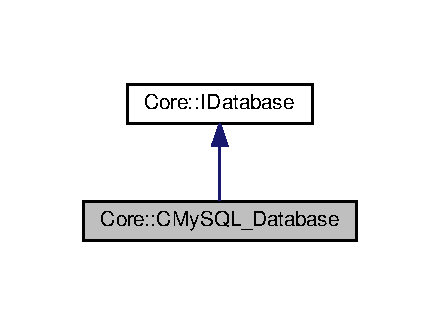
\includegraphics[width=211pt]{classCore_1_1CMySQL__Database__inherit__graph}
\end{center}
\end{figure}


Collaboration diagram for Core\+:\+:C\+My\+S\+Q\+L\+\_\+\+Database\+:\nopagebreak
\begin{figure}[H]
\begin{center}
\leavevmode
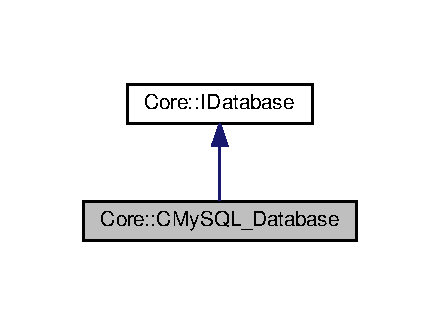
\includegraphics[width=211pt]{classCore_1_1CMySQL__Database__coll__graph}
\end{center}
\end{figure}
\subsection*{Public Member Functions}
\begin{DoxyCompactItemize}
\item 
\hyperlink{classCore_1_1CMySQL__Database_a37cbb9051d1a66753a8230bfb2f84f5e}{C\+My\+S\+Q\+L\+\_\+\+Database} ()
\item 
\hyperlink{classCore_1_1CMySQL__Database_a53a4d1a974841dbb5c5e5fe00d7f2949}{C\+My\+S\+Q\+L\+\_\+\+Database} (std\+::string \+\_\+host, std\+::string \+\_\+database, std\+::string \+\_\+user, std\+::string \+\_\+password)
\item 
virtual \hyperlink{classCore_1_1CMySQL__Database_a2d5a1c5d996209c8a13a276e931703c8}{$\sim$\+C\+My\+S\+Q\+L\+\_\+\+Database} ()
\item 
virtual void \hyperlink{classCore_1_1CMySQL__Database_a4dd288c35b1606b4ae105b968e0f9e9d}{Connect} (std\+::string \+\_\+host, std\+::string \+\_\+database, std\+::string \+\_\+user, std\+::string \+\_\+password)
\item 
virtual void \hyperlink{classCore_1_1CMySQL__Database_a1341fb3ef4974c6f4990334e409cd472}{Q\+Execute} (std\+::string \+\_\+query)
\item 
virtual std\+::unique\+\_\+ptr$<$ \hyperlink{classCore_1_1IResult}{I\+Result} $>$ \hyperlink{classCore_1_1CMySQL__Database_ab6b2e371bfde191cb00f98d29434e256}{Q\+Store} (std\+::string \+\_\+query)
\end{DoxyCompactItemize}


\subsection{Constructor \& Destructor Documentation}
\index{Core\+::\+C\+My\+S\+Q\+L\+\_\+\+Database@{Core\+::\+C\+My\+S\+Q\+L\+\_\+\+Database}!C\+My\+S\+Q\+L\+\_\+\+Database@{C\+My\+S\+Q\+L\+\_\+\+Database}}
\index{C\+My\+S\+Q\+L\+\_\+\+Database@{C\+My\+S\+Q\+L\+\_\+\+Database}!Core\+::\+C\+My\+S\+Q\+L\+\_\+\+Database@{Core\+::\+C\+My\+S\+Q\+L\+\_\+\+Database}}
\subsubsection[{\texorpdfstring{C\+My\+S\+Q\+L\+\_\+\+Database()}{CMySQL_Database()}}]{\setlength{\rightskip}{0pt plus 5cm}Core\+::\+C\+My\+S\+Q\+L\+\_\+\+Database\+::\+C\+My\+S\+Q\+L\+\_\+\+Database (
\begin{DoxyParamCaption}
{}
\end{DoxyParamCaption}
)}\hypertarget{classCore_1_1CMySQL__Database_a37cbb9051d1a66753a8230bfb2f84f5e}{}\label{classCore_1_1CMySQL__Database_a37cbb9051d1a66753a8230bfb2f84f5e}
\index{Core\+::\+C\+My\+S\+Q\+L\+\_\+\+Database@{Core\+::\+C\+My\+S\+Q\+L\+\_\+\+Database}!C\+My\+S\+Q\+L\+\_\+\+Database@{C\+My\+S\+Q\+L\+\_\+\+Database}}
\index{C\+My\+S\+Q\+L\+\_\+\+Database@{C\+My\+S\+Q\+L\+\_\+\+Database}!Core\+::\+C\+My\+S\+Q\+L\+\_\+\+Database@{Core\+::\+C\+My\+S\+Q\+L\+\_\+\+Database}}
\subsubsection[{\texorpdfstring{C\+My\+S\+Q\+L\+\_\+\+Database(std\+::string \+\_\+host, std\+::string \+\_\+database, std\+::string \+\_\+user, std\+::string \+\_\+password)}{CMySQL_Database(std::string _host, std::string _database, std::string _user, std::string _password)}}]{\setlength{\rightskip}{0pt plus 5cm}Core\+::\+C\+My\+S\+Q\+L\+\_\+\+Database\+::\+C\+My\+S\+Q\+L\+\_\+\+Database (
\begin{DoxyParamCaption}
\item[{std\+::string}]{\+\_\+host, }
\item[{std\+::string}]{\+\_\+database, }
\item[{std\+::string}]{\+\_\+user, }
\item[{std\+::string}]{\+\_\+password}
\end{DoxyParamCaption}
)}\hypertarget{classCore_1_1CMySQL__Database_a53a4d1a974841dbb5c5e5fe00d7f2949}{}\label{classCore_1_1CMySQL__Database_a53a4d1a974841dbb5c5e5fe00d7f2949}
\index{Core\+::\+C\+My\+S\+Q\+L\+\_\+\+Database@{Core\+::\+C\+My\+S\+Q\+L\+\_\+\+Database}!````~C\+My\+S\+Q\+L\+\_\+\+Database@{$\sim$\+C\+My\+S\+Q\+L\+\_\+\+Database}}
\index{````~C\+My\+S\+Q\+L\+\_\+\+Database@{$\sim$\+C\+My\+S\+Q\+L\+\_\+\+Database}!Core\+::\+C\+My\+S\+Q\+L\+\_\+\+Database@{Core\+::\+C\+My\+S\+Q\+L\+\_\+\+Database}}
\subsubsection[{\texorpdfstring{$\sim$\+C\+My\+S\+Q\+L\+\_\+\+Database()}{~CMySQL_Database()}}]{\setlength{\rightskip}{0pt plus 5cm}Core\+::\+C\+My\+S\+Q\+L\+\_\+\+Database\+::$\sim$\+C\+My\+S\+Q\+L\+\_\+\+Database (
\begin{DoxyParamCaption}
{}
\end{DoxyParamCaption}
)\hspace{0.3cm}{\ttfamily [virtual]}}\hypertarget{classCore_1_1CMySQL__Database_a2d5a1c5d996209c8a13a276e931703c8}{}\label{classCore_1_1CMySQL__Database_a2d5a1c5d996209c8a13a276e931703c8}


\subsection{Member Function Documentation}
\index{Core\+::\+C\+My\+S\+Q\+L\+\_\+\+Database@{Core\+::\+C\+My\+S\+Q\+L\+\_\+\+Database}!Connect@{Connect}}
\index{Connect@{Connect}!Core\+::\+C\+My\+S\+Q\+L\+\_\+\+Database@{Core\+::\+C\+My\+S\+Q\+L\+\_\+\+Database}}
\subsubsection[{\texorpdfstring{Connect(std\+::string \+\_\+host, std\+::string \+\_\+database, std\+::string \+\_\+user, std\+::string \+\_\+password)}{Connect(std::string _host, std::string _database, std::string _user, std::string _password)}}]{\setlength{\rightskip}{0pt plus 5cm}void Core\+::\+C\+My\+S\+Q\+L\+\_\+\+Database\+::\+Connect (
\begin{DoxyParamCaption}
\item[{std\+::string}]{\+\_\+host, }
\item[{std\+::string}]{\+\_\+database, }
\item[{std\+::string}]{\+\_\+user, }
\item[{std\+::string}]{\+\_\+password}
\end{DoxyParamCaption}
)\hspace{0.3cm}{\ttfamily [virtual]}}\hypertarget{classCore_1_1CMySQL__Database_a4dd288c35b1606b4ae105b968e0f9e9d}{}\label{classCore_1_1CMySQL__Database_a4dd288c35b1606b4ae105b968e0f9e9d}


Implements \hyperlink{classCore_1_1IDatabase_ae44631affbe063b1874a24d8c5bfa7a1}{Core\+::\+I\+Database}.

\index{Core\+::\+C\+My\+S\+Q\+L\+\_\+\+Database@{Core\+::\+C\+My\+S\+Q\+L\+\_\+\+Database}!Q\+Execute@{Q\+Execute}}
\index{Q\+Execute@{Q\+Execute}!Core\+::\+C\+My\+S\+Q\+L\+\_\+\+Database@{Core\+::\+C\+My\+S\+Q\+L\+\_\+\+Database}}
\subsubsection[{\texorpdfstring{Q\+Execute(std\+::string \+\_\+query)}{QExecute(std::string _query)}}]{\setlength{\rightskip}{0pt plus 5cm}void Core\+::\+C\+My\+S\+Q\+L\+\_\+\+Database\+::\+Q\+Execute (
\begin{DoxyParamCaption}
\item[{std\+::string}]{\+\_\+query}
\end{DoxyParamCaption}
)\hspace{0.3cm}{\ttfamily [virtual]}}\hypertarget{classCore_1_1CMySQL__Database_a1341fb3ef4974c6f4990334e409cd472}{}\label{classCore_1_1CMySQL__Database_a1341fb3ef4974c6f4990334e409cd472}


Implements \hyperlink{classCore_1_1IDatabase_a4c99cdc857e6177f6dcbb20ec4991885}{Core\+::\+I\+Database}.

\index{Core\+::\+C\+My\+S\+Q\+L\+\_\+\+Database@{Core\+::\+C\+My\+S\+Q\+L\+\_\+\+Database}!Q\+Store@{Q\+Store}}
\index{Q\+Store@{Q\+Store}!Core\+::\+C\+My\+S\+Q\+L\+\_\+\+Database@{Core\+::\+C\+My\+S\+Q\+L\+\_\+\+Database}}
\subsubsection[{\texorpdfstring{Q\+Store(std\+::string \+\_\+query)}{QStore(std::string _query)}}]{\setlength{\rightskip}{0pt plus 5cm}std\+::unique\+\_\+ptr$<$ {\bf I\+Result} $>$ Core\+::\+C\+My\+S\+Q\+L\+\_\+\+Database\+::\+Q\+Store (
\begin{DoxyParamCaption}
\item[{std\+::string}]{\+\_\+query}
\end{DoxyParamCaption}
)\hspace{0.3cm}{\ttfamily [virtual]}}\hypertarget{classCore_1_1CMySQL__Database_ab6b2e371bfde191cb00f98d29434e256}{}\label{classCore_1_1CMySQL__Database_ab6b2e371bfde191cb00f98d29434e256}


Implements \hyperlink{classCore_1_1IDatabase_aef93e70d32f2604712bf6439511f3485}{Core\+::\+I\+Database}.



The documentation for this class was generated from the following files\+:\begin{DoxyCompactItemize}
\item 
\hyperlink{cmysql__database_8h}{cmysql\+\_\+database.\+h}\item 
\hyperlink{cmysql__database_8cpp}{cmysql\+\_\+database.\+cpp}\end{DoxyCompactItemize}

\hypertarget{classCore_1_1CMySQL__Result}{}\section{Core\+:\+:C\+My\+S\+Q\+L\+\_\+\+Result Class Reference}
\label{classCore_1_1CMySQL__Result}\index{Core\+::\+C\+My\+S\+Q\+L\+\_\+\+Result@{Core\+::\+C\+My\+S\+Q\+L\+\_\+\+Result}}


{\ttfamily \#include $<$core/include/cmysql\+\_\+database.\+h$>$}



Inheritance diagram for Core\+:\+:C\+My\+S\+Q\+L\+\_\+\+Result\+:\nopagebreak
\begin{figure}[H]
\begin{center}
\leavevmode
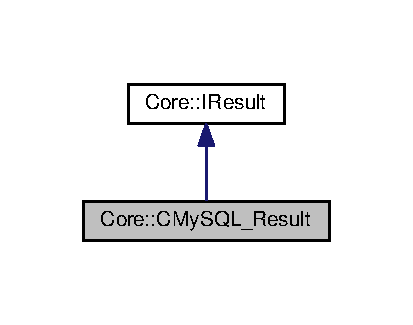
\includegraphics[width=198pt]{classCore_1_1CMySQL__Result__inherit__graph}
\end{center}
\end{figure}


Collaboration diagram for Core\+:\+:C\+My\+S\+Q\+L\+\_\+\+Result\+:\nopagebreak
\begin{figure}[H]
\begin{center}
\leavevmode
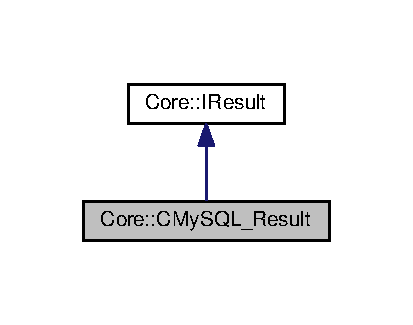
\includegraphics[width=198pt]{classCore_1_1CMySQL__Result__coll__graph}
\end{center}
\end{figure}
\subsection*{Public Member Functions}
\begin{DoxyCompactItemize}
\item 
\hyperlink{classCore_1_1CMySQL__Result_a38f36961f586d9c7763300c88aa85a9c}{C\+My\+S\+Q\+L\+\_\+\+Result} (const mysqlpp\+::\+Store\+Query\+Result \&)
\item 
virtual \hyperlink{classCore_1_1CMySQL__Result_a6237ebfb0438d571b713a62606ad0f5c}{$\sim$\+C\+My\+S\+Q\+L\+\_\+\+Result} ()
\item 
virtual bool \hyperlink{classCore_1_1CMySQL__Result_a432de24b42bb64ff4eb082ee6db97d52}{increment\+Row} ()
\item 
virtual uint32\+\_\+t \hyperlink{classCore_1_1CMySQL__Result_af5e5f0783f0ee7e09ae508bb81176bb8}{size} () const 
\item 
virtual bool \hyperlink{classCore_1_1CMySQL__Result_a839fa1572ea7a20041ec8b5181017e80}{get\+String} (std\+::string const \&column\+Name, std\+::string \&data)
\item 
virtual bool \hyperlink{classCore_1_1CMySQL__Result_add098e59d4e53d790a8934acc64543e8}{get\+Int} (std\+::string const \&column\+Name, uint32\+\_\+t \&data)
\item 
virtual bool \hyperlink{classCore_1_1CMySQL__Result_aa3d600b73235197ae49926fdc726e1a2}{get\+Float} (std\+::string const \&column\+Name, float \&data)
\end{DoxyCompactItemize}
\subsection*{Additional Inherited Members}


\subsection{Constructor \& Destructor Documentation}
\index{Core\+::\+C\+My\+S\+Q\+L\+\_\+\+Result@{Core\+::\+C\+My\+S\+Q\+L\+\_\+\+Result}!C\+My\+S\+Q\+L\+\_\+\+Result@{C\+My\+S\+Q\+L\+\_\+\+Result}}
\index{C\+My\+S\+Q\+L\+\_\+\+Result@{C\+My\+S\+Q\+L\+\_\+\+Result}!Core\+::\+C\+My\+S\+Q\+L\+\_\+\+Result@{Core\+::\+C\+My\+S\+Q\+L\+\_\+\+Result}}
\subsubsection[{\texorpdfstring{C\+My\+S\+Q\+L\+\_\+\+Result(const mysqlpp\+::\+Store\+Query\+Result \&)}{CMySQL_Result(const mysqlpp::StoreQueryResult &)}}]{\setlength{\rightskip}{0pt plus 5cm}Core\+::\+C\+My\+S\+Q\+L\+\_\+\+Result\+::\+C\+My\+S\+Q\+L\+\_\+\+Result (
\begin{DoxyParamCaption}
\item[{const mysqlpp\+::\+Store\+Query\+Result \&}]{\+\_\+res}
\end{DoxyParamCaption}
)}\hypertarget{classCore_1_1CMySQL__Result_a38f36961f586d9c7763300c88aa85a9c}{}\label{classCore_1_1CMySQL__Result_a38f36961f586d9c7763300c88aa85a9c}
\index{Core\+::\+C\+My\+S\+Q\+L\+\_\+\+Result@{Core\+::\+C\+My\+S\+Q\+L\+\_\+\+Result}!````~C\+My\+S\+Q\+L\+\_\+\+Result@{$\sim$\+C\+My\+S\+Q\+L\+\_\+\+Result}}
\index{````~C\+My\+S\+Q\+L\+\_\+\+Result@{$\sim$\+C\+My\+S\+Q\+L\+\_\+\+Result}!Core\+::\+C\+My\+S\+Q\+L\+\_\+\+Result@{Core\+::\+C\+My\+S\+Q\+L\+\_\+\+Result}}
\subsubsection[{\texorpdfstring{$\sim$\+C\+My\+S\+Q\+L\+\_\+\+Result()}{~CMySQL_Result()}}]{\setlength{\rightskip}{0pt plus 5cm}virtual Core\+::\+C\+My\+S\+Q\+L\+\_\+\+Result\+::$\sim$\+C\+My\+S\+Q\+L\+\_\+\+Result (
\begin{DoxyParamCaption}
{}
\end{DoxyParamCaption}
)\hspace{0.3cm}{\ttfamily [inline]}, {\ttfamily [virtual]}}\hypertarget{classCore_1_1CMySQL__Result_a6237ebfb0438d571b713a62606ad0f5c}{}\label{classCore_1_1CMySQL__Result_a6237ebfb0438d571b713a62606ad0f5c}


\subsection{Member Function Documentation}
\index{Core\+::\+C\+My\+S\+Q\+L\+\_\+\+Result@{Core\+::\+C\+My\+S\+Q\+L\+\_\+\+Result}!get\+Float@{get\+Float}}
\index{get\+Float@{get\+Float}!Core\+::\+C\+My\+S\+Q\+L\+\_\+\+Result@{Core\+::\+C\+My\+S\+Q\+L\+\_\+\+Result}}
\subsubsection[{\texorpdfstring{get\+Float(std\+::string const \&column\+Name, float \&data)}{getFloat(std::string const &columnName, float &data)}}]{\setlength{\rightskip}{0pt plus 5cm}bool Core\+::\+C\+My\+S\+Q\+L\+\_\+\+Result\+::get\+Float (
\begin{DoxyParamCaption}
\item[{std\+::string const \&}]{column\+Name, }
\item[{float \&}]{data}
\end{DoxyParamCaption}
)\hspace{0.3cm}{\ttfamily [virtual]}}\hypertarget{classCore_1_1CMySQL__Result_aa3d600b73235197ae49926fdc726e1a2}{}\label{classCore_1_1CMySQL__Result_aa3d600b73235197ae49926fdc726e1a2}


Implements \hyperlink{classCore_1_1IResult_a32e076c5c5ba522e4c58095637fe0f3e}{Core\+::\+I\+Result}.

\index{Core\+::\+C\+My\+S\+Q\+L\+\_\+\+Result@{Core\+::\+C\+My\+S\+Q\+L\+\_\+\+Result}!get\+Int@{get\+Int}}
\index{get\+Int@{get\+Int}!Core\+::\+C\+My\+S\+Q\+L\+\_\+\+Result@{Core\+::\+C\+My\+S\+Q\+L\+\_\+\+Result}}
\subsubsection[{\texorpdfstring{get\+Int(std\+::string const \&column\+Name, uint32\+\_\+t \&data)}{getInt(std::string const &columnName, uint32_t &data)}}]{\setlength{\rightskip}{0pt plus 5cm}bool Core\+::\+C\+My\+S\+Q\+L\+\_\+\+Result\+::get\+Int (
\begin{DoxyParamCaption}
\item[{std\+::string const \&}]{column\+Name, }
\item[{uint32\+\_\+t \&}]{data}
\end{DoxyParamCaption}
)\hspace{0.3cm}{\ttfamily [virtual]}}\hypertarget{classCore_1_1CMySQL__Result_add098e59d4e53d790a8934acc64543e8}{}\label{classCore_1_1CMySQL__Result_add098e59d4e53d790a8934acc64543e8}


Implements \hyperlink{classCore_1_1IResult_a9c01330c5b826ca948b48e13a330f4cd}{Core\+::\+I\+Result}.

\index{Core\+::\+C\+My\+S\+Q\+L\+\_\+\+Result@{Core\+::\+C\+My\+S\+Q\+L\+\_\+\+Result}!get\+String@{get\+String}}
\index{get\+String@{get\+String}!Core\+::\+C\+My\+S\+Q\+L\+\_\+\+Result@{Core\+::\+C\+My\+S\+Q\+L\+\_\+\+Result}}
\subsubsection[{\texorpdfstring{get\+String(std\+::string const \&column\+Name, std\+::string \&data)}{getString(std::string const &columnName, std::string &data)}}]{\setlength{\rightskip}{0pt plus 5cm}bool Core\+::\+C\+My\+S\+Q\+L\+\_\+\+Result\+::get\+String (
\begin{DoxyParamCaption}
\item[{std\+::string const \&}]{column\+Name, }
\item[{std\+::string \&}]{data}
\end{DoxyParamCaption}
)\hspace{0.3cm}{\ttfamily [virtual]}}\hypertarget{classCore_1_1CMySQL__Result_a839fa1572ea7a20041ec8b5181017e80}{}\label{classCore_1_1CMySQL__Result_a839fa1572ea7a20041ec8b5181017e80}


Implements \hyperlink{classCore_1_1IResult_a6b96b8324d81a1a65d60a4f6a6e78052}{Core\+::\+I\+Result}.

\index{Core\+::\+C\+My\+S\+Q\+L\+\_\+\+Result@{Core\+::\+C\+My\+S\+Q\+L\+\_\+\+Result}!increment\+Row@{increment\+Row}}
\index{increment\+Row@{increment\+Row}!Core\+::\+C\+My\+S\+Q\+L\+\_\+\+Result@{Core\+::\+C\+My\+S\+Q\+L\+\_\+\+Result}}
\subsubsection[{\texorpdfstring{increment\+Row()}{incrementRow()}}]{\setlength{\rightskip}{0pt plus 5cm}bool Core\+::\+C\+My\+S\+Q\+L\+\_\+\+Result\+::increment\+Row (
\begin{DoxyParamCaption}
{}
\end{DoxyParamCaption}
)\hspace{0.3cm}{\ttfamily [virtual]}}\hypertarget{classCore_1_1CMySQL__Result_a432de24b42bb64ff4eb082ee6db97d52}{}\label{classCore_1_1CMySQL__Result_a432de24b42bb64ff4eb082ee6db97d52}


Reimplemented from \hyperlink{classCore_1_1IResult_a93fe49ee2a9ab7ed520293d9e1339a96}{Core\+::\+I\+Result}.

\index{Core\+::\+C\+My\+S\+Q\+L\+\_\+\+Result@{Core\+::\+C\+My\+S\+Q\+L\+\_\+\+Result}!size@{size}}
\index{size@{size}!Core\+::\+C\+My\+S\+Q\+L\+\_\+\+Result@{Core\+::\+C\+My\+S\+Q\+L\+\_\+\+Result}}
\subsubsection[{\texorpdfstring{size() const }{size() const }}]{\setlength{\rightskip}{0pt plus 5cm}virtual uint32\+\_\+t Core\+::\+C\+My\+S\+Q\+L\+\_\+\+Result\+::size (
\begin{DoxyParamCaption}
{}
\end{DoxyParamCaption}
) const\hspace{0.3cm}{\ttfamily [inline]}, {\ttfamily [virtual]}}\hypertarget{classCore_1_1CMySQL__Result_af5e5f0783f0ee7e09ae508bb81176bb8}{}\label{classCore_1_1CMySQL__Result_af5e5f0783f0ee7e09ae508bb81176bb8}


Implements \hyperlink{classCore_1_1IResult_a308ce2382287ba5de5102fc532097709}{Core\+::\+I\+Result}.



The documentation for this class was generated from the following files\+:\begin{DoxyCompactItemize}
\item 
\hyperlink{cmysql__database_8h}{cmysql\+\_\+database.\+h}\item 
\hyperlink{cmysql__database_8cpp}{cmysql\+\_\+database.\+cpp}\end{DoxyCompactItemize}

\hypertarget{classCore_1_1CMySQL__Row}{}\section{Core\+:\+:C\+My\+S\+Q\+L\+\_\+\+Row Class Reference}
\label{classCore_1_1CMySQL__Row}\index{Core\+::\+C\+My\+S\+Q\+L\+\_\+\+Row@{Core\+::\+C\+My\+S\+Q\+L\+\_\+\+Row}}


{\ttfamily \#include $<$core/include/cmysql\+\_\+database.\+h$>$}



Inheritance diagram for Core\+:\+:C\+My\+S\+Q\+L\+\_\+\+Row\+:\nopagebreak
\begin{figure}[H]
\begin{center}
\leavevmode
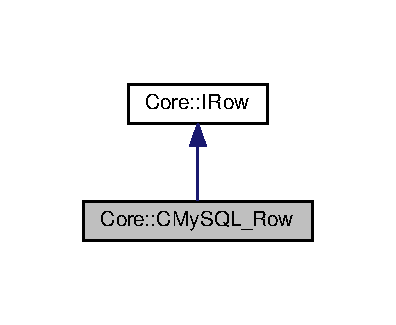
\includegraphics[width=190pt]{classCore_1_1CMySQL__Row__inherit__graph}
\end{center}
\end{figure}


Collaboration diagram for Core\+:\+:C\+My\+S\+Q\+L\+\_\+\+Row\+:\nopagebreak
\begin{figure}[H]
\begin{center}
\leavevmode
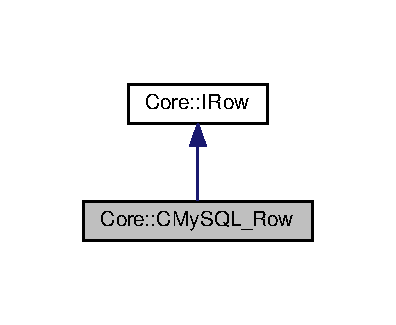
\includegraphics[width=190pt]{classCore_1_1CMySQL__Row__coll__graph}
\end{center}
\end{figure}
\subsection*{Public Member Functions}
\begin{DoxyCompactItemize}
\item 
\hyperlink{classCore_1_1CMySQL__Row_acc5448d29db4d50e25a4b5ca8d9c531d}{C\+My\+S\+Q\+L\+\_\+\+Row} (const mysqlpp\+::\+Row \&row)
\item 
virtual \hyperlink{classCore_1_1CMySQL__Row_a66cd53072a76eac953e990246eb5378a}{$\sim$\+C\+My\+S\+Q\+L\+\_\+\+Row} ()
\item 
virtual bool \hyperlink{classCore_1_1CMySQL__Row_a6eefe9e7854e34c4e17eb57b61fa125e}{get\+String} (std\+::string const \&column\+Name, std\+::string \&data)
\item 
virtual bool \hyperlink{classCore_1_1CMySQL__Row_a474e2628522f15c955d0a17747007c13}{get\+Int} (std\+::string const \&column\+Name, uint32\+\_\+t \&data)
\item 
virtual bool \hyperlink{classCore_1_1CMySQL__Row_a1d1f5caf4a767dfe97d8d6da08d1ff1b}{get\+Float} (std\+::string const \&column\+Name, float \&data)
\end{DoxyCompactItemize}


\subsection{Constructor \& Destructor Documentation}
\index{Core\+::\+C\+My\+S\+Q\+L\+\_\+\+Row@{Core\+::\+C\+My\+S\+Q\+L\+\_\+\+Row}!C\+My\+S\+Q\+L\+\_\+\+Row@{C\+My\+S\+Q\+L\+\_\+\+Row}}
\index{C\+My\+S\+Q\+L\+\_\+\+Row@{C\+My\+S\+Q\+L\+\_\+\+Row}!Core\+::\+C\+My\+S\+Q\+L\+\_\+\+Row@{Core\+::\+C\+My\+S\+Q\+L\+\_\+\+Row}}
\subsubsection[{\texorpdfstring{C\+My\+S\+Q\+L\+\_\+\+Row(const mysqlpp\+::\+Row \&row)}{CMySQL_Row(const mysqlpp::Row &row)}}]{\setlength{\rightskip}{0pt plus 5cm}Core\+::\+C\+My\+S\+Q\+L\+\_\+\+Row\+::\+C\+My\+S\+Q\+L\+\_\+\+Row (
\begin{DoxyParamCaption}
\item[{const mysqlpp\+::\+Row \&}]{row}
\end{DoxyParamCaption}
)\hspace{0.3cm}{\ttfamily [inline]}}\hypertarget{classCore_1_1CMySQL__Row_acc5448d29db4d50e25a4b5ca8d9c531d}{}\label{classCore_1_1CMySQL__Row_acc5448d29db4d50e25a4b5ca8d9c531d}
\index{Core\+::\+C\+My\+S\+Q\+L\+\_\+\+Row@{Core\+::\+C\+My\+S\+Q\+L\+\_\+\+Row}!````~C\+My\+S\+Q\+L\+\_\+\+Row@{$\sim$\+C\+My\+S\+Q\+L\+\_\+\+Row}}
\index{````~C\+My\+S\+Q\+L\+\_\+\+Row@{$\sim$\+C\+My\+S\+Q\+L\+\_\+\+Row}!Core\+::\+C\+My\+S\+Q\+L\+\_\+\+Row@{Core\+::\+C\+My\+S\+Q\+L\+\_\+\+Row}}
\subsubsection[{\texorpdfstring{$\sim$\+C\+My\+S\+Q\+L\+\_\+\+Row()}{~CMySQL_Row()}}]{\setlength{\rightskip}{0pt plus 5cm}virtual Core\+::\+C\+My\+S\+Q\+L\+\_\+\+Row\+::$\sim$\+C\+My\+S\+Q\+L\+\_\+\+Row (
\begin{DoxyParamCaption}
{}
\end{DoxyParamCaption}
)\hspace{0.3cm}{\ttfamily [inline]}, {\ttfamily [virtual]}}\hypertarget{classCore_1_1CMySQL__Row_a66cd53072a76eac953e990246eb5378a}{}\label{classCore_1_1CMySQL__Row_a66cd53072a76eac953e990246eb5378a}


\subsection{Member Function Documentation}
\index{Core\+::\+C\+My\+S\+Q\+L\+\_\+\+Row@{Core\+::\+C\+My\+S\+Q\+L\+\_\+\+Row}!get\+Float@{get\+Float}}
\index{get\+Float@{get\+Float}!Core\+::\+C\+My\+S\+Q\+L\+\_\+\+Row@{Core\+::\+C\+My\+S\+Q\+L\+\_\+\+Row}}
\subsubsection[{\texorpdfstring{get\+Float(std\+::string const \&column\+Name, float \&data)}{getFloat(std::string const &columnName, float &data)}}]{\setlength{\rightskip}{0pt plus 5cm}bool Core\+::\+C\+My\+S\+Q\+L\+\_\+\+Row\+::get\+Float (
\begin{DoxyParamCaption}
\item[{std\+::string const \&}]{column\+Name, }
\item[{float \&}]{data}
\end{DoxyParamCaption}
)\hspace{0.3cm}{\ttfamily [virtual]}}\hypertarget{classCore_1_1CMySQL__Row_a1d1f5caf4a767dfe97d8d6da08d1ff1b}{}\label{classCore_1_1CMySQL__Row_a1d1f5caf4a767dfe97d8d6da08d1ff1b}


Implements \hyperlink{classCore_1_1IRow_a8cc28cd6cc7902d7a1fb5b68cca1b1c8}{Core\+::\+I\+Row}.

\index{Core\+::\+C\+My\+S\+Q\+L\+\_\+\+Row@{Core\+::\+C\+My\+S\+Q\+L\+\_\+\+Row}!get\+Int@{get\+Int}}
\index{get\+Int@{get\+Int}!Core\+::\+C\+My\+S\+Q\+L\+\_\+\+Row@{Core\+::\+C\+My\+S\+Q\+L\+\_\+\+Row}}
\subsubsection[{\texorpdfstring{get\+Int(std\+::string const \&column\+Name, uint32\+\_\+t \&data)}{getInt(std::string const &columnName, uint32_t &data)}}]{\setlength{\rightskip}{0pt plus 5cm}bool Core\+::\+C\+My\+S\+Q\+L\+\_\+\+Row\+::get\+Int (
\begin{DoxyParamCaption}
\item[{std\+::string const \&}]{column\+Name, }
\item[{uint32\+\_\+t \&}]{data}
\end{DoxyParamCaption}
)\hspace{0.3cm}{\ttfamily [virtual]}}\hypertarget{classCore_1_1CMySQL__Row_a474e2628522f15c955d0a17747007c13}{}\label{classCore_1_1CMySQL__Row_a474e2628522f15c955d0a17747007c13}


Implements \hyperlink{classCore_1_1IRow_aa90ad0d42f61cc3101b8b13b389eb5b3}{Core\+::\+I\+Row}.

\index{Core\+::\+C\+My\+S\+Q\+L\+\_\+\+Row@{Core\+::\+C\+My\+S\+Q\+L\+\_\+\+Row}!get\+String@{get\+String}}
\index{get\+String@{get\+String}!Core\+::\+C\+My\+S\+Q\+L\+\_\+\+Row@{Core\+::\+C\+My\+S\+Q\+L\+\_\+\+Row}}
\subsubsection[{\texorpdfstring{get\+String(std\+::string const \&column\+Name, std\+::string \&data)}{getString(std::string const &columnName, std::string &data)}}]{\setlength{\rightskip}{0pt plus 5cm}bool Core\+::\+C\+My\+S\+Q\+L\+\_\+\+Row\+::get\+String (
\begin{DoxyParamCaption}
\item[{std\+::string const \&}]{column\+Name, }
\item[{std\+::string \&}]{data}
\end{DoxyParamCaption}
)\hspace{0.3cm}{\ttfamily [virtual]}}\hypertarget{classCore_1_1CMySQL__Row_a6eefe9e7854e34c4e17eb57b61fa125e}{}\label{classCore_1_1CMySQL__Row_a6eefe9e7854e34c4e17eb57b61fa125e}


Implements \hyperlink{classCore_1_1IRow_a6237dc736cc99b00880ef0d8df2544ff}{Core\+::\+I\+Row}.



The documentation for this class was generated from the following files\+:\begin{DoxyCompactItemize}
\item 
\hyperlink{cmysql__database_8h}{cmysql\+\_\+database.\+h}\item 
\hyperlink{cmysql__database_8cpp}{cmysql\+\_\+database.\+cpp}\end{DoxyCompactItemize}

\hypertarget{classCore_1_1CNetwork__Asio}{}\section{Core\+:\+:C\+Network\+\_\+\+Asio Class Reference}
\label{classCore_1_1CNetwork__Asio}\index{Core\+::\+C\+Network\+\_\+\+Asio@{Core\+::\+C\+Network\+\_\+\+Asio}}


{\ttfamily \#include $<$core/include/cnetwork\+\_\+asio.\+h$>$}



Inheritance diagram for Core\+:\+:C\+Network\+\_\+\+Asio\+:\nopagebreak
\begin{figure}[H]
\begin{center}
\leavevmode
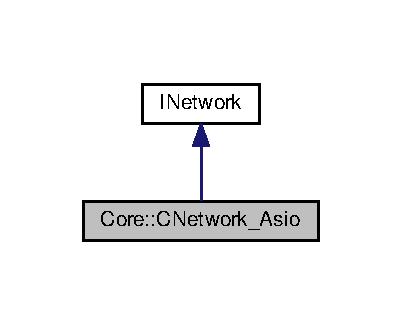
\includegraphics[width=193pt]{classCore_1_1CNetwork__Asio__inherit__graph}
\end{center}
\end{figure}


Collaboration diagram for Core\+:\+:C\+Network\+\_\+\+Asio\+:\nopagebreak
\begin{figure}[H]
\begin{center}
\leavevmode
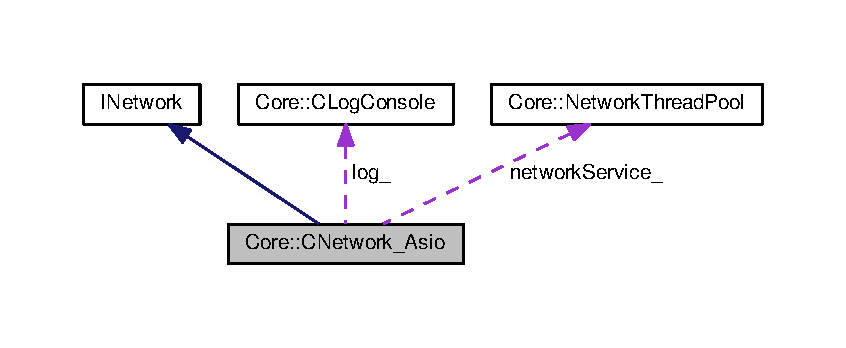
\includegraphics[width=350pt]{classCore_1_1CNetwork__Asio__coll__graph}
\end{center}
\end{figure}
\subsection*{Public Member Functions}
\begin{DoxyCompactItemize}
\item 
\hyperlink{classCore_1_1CNetwork__Asio_a9ef0f93160b19262ebad0ebc42f8c910}{C\+Network\+\_\+\+Asio} ()
\item 
virtual \hyperlink{classCore_1_1CNetwork__Asio_a642030ea5baa0f3a5b08a73dfdc4df79}{$\sim$\+C\+Network\+\_\+\+Asio} ()
\item 
virtual bool \hyperlink{classCore_1_1CNetwork__Asio_a6510dd6c07d2de995242f9ea827b97d1}{Init} (std\+::string \+\_\+ip, uint16\+\_\+t \+\_\+port)
\item 
virtual bool \hyperlink{classCore_1_1CNetwork__Asio_a1990de08bdc733e76d575f13b03072d0}{Shutdown} ()
\item 
virtual bool \hyperlink{classCore_1_1CNetwork__Asio_a126de0c3a03d6f2efe21f2b1888285b4}{Connect} ()
\item 
virtual bool \hyperlink{classCore_1_1CNetwork__Asio_accbfdbf25e902928bbe3809307510505}{Listen} ()
\item 
virtual bool \hyperlink{classCore_1_1CNetwork__Asio_a57f1ef8e8849990b393b27fcece6871d}{Reconnect} ()
\item 
virtual bool \hyperlink{classCore_1_1CNetwork__Asio_aa98b86ad1ade6a4de084577a30b6d6d4}{Disconnect} ()
\item 
virtual bool \hyperlink{classCore_1_1CNetwork__Asio_a2f84428ff2250e960ba2739b45f491a2}{Send} (std\+::unique\+\_\+ptr$<$ uint8\+\_\+t $>$ \+\_\+buffer)
\item 
virtual bool \hyperlink{classCore_1_1CNetwork__Asio_a08865b2606dcef0e38f27532b1ae3909}{Recv} (uint16\+\_\+t \+\_\+size=\hyperlink{cnetwork__asio_8h_a879456c3b8e2853f7044d764e9c180d4}{M\+A\+X\+\_\+\+P\+A\+C\+K\+E\+T\+\_\+\+S\+I\+ZE})
\item 
bool \hyperlink{classCore_1_1CNetwork__Asio_a0529c15321b8065795b692d2da8830a6}{Is\+Active} ()
\item 
void \hyperlink{classCore_1_1CNetwork__Asio_ad2664e347338dc680ba117f896c759b5}{Set\+Extra\+Message\+Info} (bool \+\_\+enabled)
\end{DoxyCompactItemize}
\subsection*{Protected Member Functions}
\begin{DoxyCompactItemize}
\item 
void \hyperlink{classCore_1_1CNetwork__Asio_a048ed61b243deed5905b89b0826f413b}{Accept\+Connection} ()
\item 
virtual bool \hyperlink{classCore_1_1CNetwork__Asio_a8b5610d420eaa22aafa429fe9d7590a9}{On\+Connect} ()
\item 
virtual void \hyperlink{classCore_1_1CNetwork__Asio_a654726debc63f13a31e8f3c0d517259e}{On\+Connected} ()
\item 
virtual bool \hyperlink{classCore_1_1CNetwork__Asio_a09c413ff854b8d8aa53b09f3eb610a34}{On\+Listen} ()
\item 
virtual void \hyperlink{classCore_1_1CNetwork__Asio_a1534e01f0aae39a12af3ac3e88aa7954}{On\+Listening} ()
\item 
virtual bool \hyperlink{classCore_1_1CNetwork__Asio_afb65283ace223c5a3bea6029b8c6a809}{On\+Disconnect} ()
\item 
virtual void \hyperlink{classCore_1_1CNetwork__Asio_a1e813736a887fe3a128b1672be1cbb10}{On\+Disconnected} ()
\item 
virtual bool \hyperlink{classCore_1_1CNetwork__Asio_af97c853ab0bcba0372919f0a243f4cb5}{On\+Receive} ()
\item 
virtual bool \hyperlink{classCore_1_1CNetwork__Asio_acb2952682b6abbce60b01d9c75b02729}{On\+Received} ()
\item 
virtual bool \hyperlink{classCore_1_1CNetwork__Asio_a3cfea157222e7ef2c1e67f2c0e25ed8c}{On\+Send} (uint8\+\_\+t $\ast$\+\_\+buffer)
\item 
virtual void \hyperlink{classCore_1_1CNetwork__Asio_a79ff0fbfb787e26a079ef259160de6e3}{On\+Sent} ()
\item 
virtual bool \hyperlink{classCore_1_1CNetwork__Asio_aa66213bfe03d098460347866bcf8a5fb}{On\+Accept} ()
\item 
virtual void \hyperlink{classCore_1_1CNetwork__Asio_a520443f28e0df2f1f38cfc685414aa98}{On\+Accepted} (tcp\+::socket \+\_\+sock)
\item 
virtual bool \hyperlink{classCore_1_1CNetwork__Asio_a8f1418b5bae79829a617fe8d0ae1a44d}{Handle\+Packet} (uint8\+\_\+t $\ast$\+\_\+buffer)
\item 
void \hyperlink{classCore_1_1CNetwork__Asio_a9d50c31ca63f017cfbdcbd97a4c8be0e}{Set\+Socket} (tcp\+::socket \+\_\+sock)
\item 
void \hyperlink{classCore_1_1CNetwork__Asio_a8781a7dee1202b6b984d25afd0002b0a}{Reset\+Buffer} ()
\end{DoxyCompactItemize}
\subsection*{Protected Attributes}
\begin{DoxyCompactItemize}
\item 
\hyperlink{classCore_1_1CLogConsole}{C\+Log\+Console} \hyperlink{classCore_1_1CNetwork__Asio_a0330ebff658531de39d4ab56ebfd3ef0}{log\+\_\+}
\item 
asio\+::io\+\_\+service $\ast$ \hyperlink{classCore_1_1CNetwork__Asio_ae8f0c7bd6d91e2c6f08b1a9c0c3d0e79}{io\+\_\+service\+\_\+}
\item 
\hyperlink{classCore_1_1NetworkThreadPool}{Core\+::\+Network\+Thread\+Pool} $\ast$ \hyperlink{classCore_1_1CNetwork__Asio_a2cd9b91538970582937b8f03df08bf4c}{network\+Service\+\_\+}
\item 
tcp\+::socket \hyperlink{classCore_1_1CNetwork__Asio_a57eebf57efe1aa1728b3e3746cde10fb}{socket\+\_\+}
\item 
tcp\+::acceptor \hyperlink{classCore_1_1CNetwork__Asio_ae41e74304ef2de1b82bc6467b13fdb6f}{listener\+\_\+}
\item 
std\+::queue$<$ std\+::unique\+\_\+ptr$<$ uint8\+\_\+t $>$ $>$ \hyperlink{classCore_1_1CNetwork__Asio_addc81f6507aaaefff55125bbd14eabae}{send\+\_\+queue\+\_\+}
\item 
std\+::queue$<$ std\+::unique\+\_\+ptr$<$ uint8\+\_\+t $>$ $>$ \hyperlink{classCore_1_1CNetwork__Asio_ade3431dccfe1d5d1faf9c539031c80be}{discard\+\_\+queue\+\_\+}
\item 
std\+::mutex \hyperlink{classCore_1_1CNetwork__Asio_a957a4eb9ab4221cf7056a902c42796f3}{send\+\_\+mutex\+\_\+}
\item 
std\+::mutex \hyperlink{classCore_1_1CNetwork__Asio_acc7289205677c219ac90c8c1445d0770}{recv\+\_\+mutex\+\_\+}
\item 
std\+::mutex \hyperlink{classCore_1_1CNetwork__Asio_a5d307130d59994026ce19f258dd31048}{discard\+\_\+mutex\+\_\+}
\item 
std\+::condition\+\_\+variable \hyperlink{classCore_1_1CNetwork__Asio_a928266d06111ae3e88fcc6608cd88cec}{recv\+\_\+condition\+\_\+}
\item 
std\+::thread \hyperlink{classCore_1_1CNetwork__Asio_a8434441ee967ff416a48f4de34e07e04}{process\+\_\+thread\+\_\+}
\item 
uint8\+\_\+t \hyperlink{classCore_1_1CNetwork__Asio_a41089e546d53aba73073ccc49cf96fd8}{buffer\+\_\+} \mbox{[}\hyperlink{cnetwork__asio_8h_a879456c3b8e2853f7044d764e9c180d4}{M\+A\+X\+\_\+\+P\+A\+C\+K\+E\+T\+\_\+\+S\+I\+ZE}\mbox{]}
\item 
uint16\+\_\+t \hyperlink{classCore_1_1CNetwork__Asio_a614aae7d1116f4dd01516e7858f3aca0}{packet\+\_\+offset\+\_\+}
\item 
uint16\+\_\+t \hyperlink{classCore_1_1CNetwork__Asio_a25301a85d636297711946f55d6664cff}{packet\+\_\+size\+\_\+}
\item 
bool \hyperlink{classCore_1_1CNetwork__Asio_abedfebd59927120d57e68b724e8431e6}{active\+\_\+}
\end{DoxyCompactItemize}


\subsection{Constructor \& Destructor Documentation}
\index{Core\+::\+C\+Network\+\_\+\+Asio@{Core\+::\+C\+Network\+\_\+\+Asio}!C\+Network\+\_\+\+Asio@{C\+Network\+\_\+\+Asio}}
\index{C\+Network\+\_\+\+Asio@{C\+Network\+\_\+\+Asio}!Core\+::\+C\+Network\+\_\+\+Asio@{Core\+::\+C\+Network\+\_\+\+Asio}}
\subsubsection[{\texorpdfstring{C\+Network\+\_\+\+Asio()}{CNetwork_Asio()}}]{\setlength{\rightskip}{0pt plus 5cm}Core\+::\+C\+Network\+\_\+\+Asio\+::\+C\+Network\+\_\+\+Asio (
\begin{DoxyParamCaption}
{}
\end{DoxyParamCaption}
)}\hypertarget{classCore_1_1CNetwork__Asio_a9ef0f93160b19262ebad0ebc42f8c910}{}\label{classCore_1_1CNetwork__Asio_a9ef0f93160b19262ebad0ebc42f8c910}
\index{Core\+::\+C\+Network\+\_\+\+Asio@{Core\+::\+C\+Network\+\_\+\+Asio}!````~C\+Network\+\_\+\+Asio@{$\sim$\+C\+Network\+\_\+\+Asio}}
\index{````~C\+Network\+\_\+\+Asio@{$\sim$\+C\+Network\+\_\+\+Asio}!Core\+::\+C\+Network\+\_\+\+Asio@{Core\+::\+C\+Network\+\_\+\+Asio}}
\subsubsection[{\texorpdfstring{$\sim$\+C\+Network\+\_\+\+Asio()}{~CNetwork_Asio()}}]{\setlength{\rightskip}{0pt plus 5cm}Core\+::\+C\+Network\+\_\+\+Asio\+::$\sim$\+C\+Network\+\_\+\+Asio (
\begin{DoxyParamCaption}
{}
\end{DoxyParamCaption}
)\hspace{0.3cm}{\ttfamily [virtual]}}\hypertarget{classCore_1_1CNetwork__Asio_a642030ea5baa0f3a5b08a73dfdc4df79}{}\label{classCore_1_1CNetwork__Asio_a642030ea5baa0f3a5b08a73dfdc4df79}


\subsection{Member Function Documentation}
\index{Core\+::\+C\+Network\+\_\+\+Asio@{Core\+::\+C\+Network\+\_\+\+Asio}!Accept\+Connection@{Accept\+Connection}}
\index{Accept\+Connection@{Accept\+Connection}!Core\+::\+C\+Network\+\_\+\+Asio@{Core\+::\+C\+Network\+\_\+\+Asio}}
\subsubsection[{\texorpdfstring{Accept\+Connection()}{AcceptConnection()}}]{\setlength{\rightskip}{0pt plus 5cm}void Core\+::\+C\+Network\+\_\+\+Asio\+::\+Accept\+Connection (
\begin{DoxyParamCaption}
{}
\end{DoxyParamCaption}
)\hspace{0.3cm}{\ttfamily [protected]}}\hypertarget{classCore_1_1CNetwork__Asio_a048ed61b243deed5905b89b0826f413b}{}\label{classCore_1_1CNetwork__Asio_a048ed61b243deed5905b89b0826f413b}
\index{Core\+::\+C\+Network\+\_\+\+Asio@{Core\+::\+C\+Network\+\_\+\+Asio}!Connect@{Connect}}
\index{Connect@{Connect}!Core\+::\+C\+Network\+\_\+\+Asio@{Core\+::\+C\+Network\+\_\+\+Asio}}
\subsubsection[{\texorpdfstring{Connect()}{Connect()}}]{\setlength{\rightskip}{0pt plus 5cm}bool Core\+::\+C\+Network\+\_\+\+Asio\+::\+Connect (
\begin{DoxyParamCaption}
{}
\end{DoxyParamCaption}
)\hspace{0.3cm}{\ttfamily [virtual]}}\hypertarget{classCore_1_1CNetwork__Asio_a126de0c3a03d6f2efe21f2b1888285b4}{}\label{classCore_1_1CNetwork__Asio_a126de0c3a03d6f2efe21f2b1888285b4}


Implements \hyperlink{classINetwork_a1b646635942e454f2f2d938bc1fb8685}{I\+Network}.

\index{Core\+::\+C\+Network\+\_\+\+Asio@{Core\+::\+C\+Network\+\_\+\+Asio}!Disconnect@{Disconnect}}
\index{Disconnect@{Disconnect}!Core\+::\+C\+Network\+\_\+\+Asio@{Core\+::\+C\+Network\+\_\+\+Asio}}
\subsubsection[{\texorpdfstring{Disconnect()}{Disconnect()}}]{\setlength{\rightskip}{0pt plus 5cm}bool Core\+::\+C\+Network\+\_\+\+Asio\+::\+Disconnect (
\begin{DoxyParamCaption}
{}
\end{DoxyParamCaption}
)\hspace{0.3cm}{\ttfamily [virtual]}}\hypertarget{classCore_1_1CNetwork__Asio_aa98b86ad1ade6a4de084577a30b6d6d4}{}\label{classCore_1_1CNetwork__Asio_aa98b86ad1ade6a4de084577a30b6d6d4}


Implements \hyperlink{classINetwork_a44726fff2e6720f61aa34e4a4ef4780d}{I\+Network}.

\index{Core\+::\+C\+Network\+\_\+\+Asio@{Core\+::\+C\+Network\+\_\+\+Asio}!Handle\+Packet@{Handle\+Packet}}
\index{Handle\+Packet@{Handle\+Packet}!Core\+::\+C\+Network\+\_\+\+Asio@{Core\+::\+C\+Network\+\_\+\+Asio}}
\subsubsection[{\texorpdfstring{Handle\+Packet(uint8\+\_\+t $\ast$\+\_\+buffer)}{HandlePacket(uint8_t *_buffer)}}]{\setlength{\rightskip}{0pt plus 5cm}bool Core\+::\+C\+Network\+\_\+\+Asio\+::\+Handle\+Packet (
\begin{DoxyParamCaption}
\item[{uint8\+\_\+t $\ast$}]{\+\_\+buffer}
\end{DoxyParamCaption}
)\hspace{0.3cm}{\ttfamily [protected]}, {\ttfamily [virtual]}}\hypertarget{classCore_1_1CNetwork__Asio_a8f1418b5bae79829a617fe8d0ae1a44d}{}\label{classCore_1_1CNetwork__Asio_a8f1418b5bae79829a617fe8d0ae1a44d}
\index{Core\+::\+C\+Network\+\_\+\+Asio@{Core\+::\+C\+Network\+\_\+\+Asio}!Init@{Init}}
\index{Init@{Init}!Core\+::\+C\+Network\+\_\+\+Asio@{Core\+::\+C\+Network\+\_\+\+Asio}}
\subsubsection[{\texorpdfstring{Init(std\+::string \+\_\+ip, uint16\+\_\+t \+\_\+port)}{Init(std::string _ip, uint16_t _port)}}]{\setlength{\rightskip}{0pt plus 5cm}bool Core\+::\+C\+Network\+\_\+\+Asio\+::\+Init (
\begin{DoxyParamCaption}
\item[{std\+::string}]{\+\_\+ip, }
\item[{uint16\+\_\+t}]{\+\_\+port}
\end{DoxyParamCaption}
)\hspace{0.3cm}{\ttfamily [virtual]}}\hypertarget{classCore_1_1CNetwork__Asio_a6510dd6c07d2de995242f9ea827b97d1}{}\label{classCore_1_1CNetwork__Asio_a6510dd6c07d2de995242f9ea827b97d1}


Implements \hyperlink{classINetwork_aff192e3d6708cb1aadef3f6667e02708}{I\+Network}.

\index{Core\+::\+C\+Network\+\_\+\+Asio@{Core\+::\+C\+Network\+\_\+\+Asio}!Is\+Active@{Is\+Active}}
\index{Is\+Active@{Is\+Active}!Core\+::\+C\+Network\+\_\+\+Asio@{Core\+::\+C\+Network\+\_\+\+Asio}}
\subsubsection[{\texorpdfstring{Is\+Active()}{IsActive()}}]{\setlength{\rightskip}{0pt plus 5cm}bool Core\+::\+C\+Network\+\_\+\+Asio\+::\+Is\+Active (
\begin{DoxyParamCaption}
{}
\end{DoxyParamCaption}
)\hspace{0.3cm}{\ttfamily [inline]}}\hypertarget{classCore_1_1CNetwork__Asio_a0529c15321b8065795b692d2da8830a6}{}\label{classCore_1_1CNetwork__Asio_a0529c15321b8065795b692d2da8830a6}
\index{Core\+::\+C\+Network\+\_\+\+Asio@{Core\+::\+C\+Network\+\_\+\+Asio}!Listen@{Listen}}
\index{Listen@{Listen}!Core\+::\+C\+Network\+\_\+\+Asio@{Core\+::\+C\+Network\+\_\+\+Asio}}
\subsubsection[{\texorpdfstring{Listen()}{Listen()}}]{\setlength{\rightskip}{0pt plus 5cm}bool Core\+::\+C\+Network\+\_\+\+Asio\+::\+Listen (
\begin{DoxyParamCaption}
{}
\end{DoxyParamCaption}
)\hspace{0.3cm}{\ttfamily [virtual]}}\hypertarget{classCore_1_1CNetwork__Asio_accbfdbf25e902928bbe3809307510505}{}\label{classCore_1_1CNetwork__Asio_accbfdbf25e902928bbe3809307510505}


Implements \hyperlink{classINetwork_a3f47952a34fec9118c26901783009ac1}{I\+Network}.

\index{Core\+::\+C\+Network\+\_\+\+Asio@{Core\+::\+C\+Network\+\_\+\+Asio}!On\+Accept@{On\+Accept}}
\index{On\+Accept@{On\+Accept}!Core\+::\+C\+Network\+\_\+\+Asio@{Core\+::\+C\+Network\+\_\+\+Asio}}
\subsubsection[{\texorpdfstring{On\+Accept()}{OnAccept()}}]{\setlength{\rightskip}{0pt plus 5cm}bool Core\+::\+C\+Network\+\_\+\+Asio\+::\+On\+Accept (
\begin{DoxyParamCaption}
{}
\end{DoxyParamCaption}
)\hspace{0.3cm}{\ttfamily [protected]}, {\ttfamily [virtual]}}\hypertarget{classCore_1_1CNetwork__Asio_aa66213bfe03d098460347866bcf8a5fb}{}\label{classCore_1_1CNetwork__Asio_aa66213bfe03d098460347866bcf8a5fb}
\index{Core\+::\+C\+Network\+\_\+\+Asio@{Core\+::\+C\+Network\+\_\+\+Asio}!On\+Accepted@{On\+Accepted}}
\index{On\+Accepted@{On\+Accepted}!Core\+::\+C\+Network\+\_\+\+Asio@{Core\+::\+C\+Network\+\_\+\+Asio}}
\subsubsection[{\texorpdfstring{On\+Accepted(tcp\+::socket \+\_\+sock)}{OnAccepted(tcp::socket _sock)}}]{\setlength{\rightskip}{0pt plus 5cm}void Core\+::\+C\+Network\+\_\+\+Asio\+::\+On\+Accepted (
\begin{DoxyParamCaption}
\item[{tcp\+::socket}]{\+\_\+sock}
\end{DoxyParamCaption}
)\hspace{0.3cm}{\ttfamily [protected]}, {\ttfamily [virtual]}}\hypertarget{classCore_1_1CNetwork__Asio_a520443f28e0df2f1f38cfc685414aa98}{}\label{classCore_1_1CNetwork__Asio_a520443f28e0df2f1f38cfc685414aa98}
\index{Core\+::\+C\+Network\+\_\+\+Asio@{Core\+::\+C\+Network\+\_\+\+Asio}!On\+Connect@{On\+Connect}}
\index{On\+Connect@{On\+Connect}!Core\+::\+C\+Network\+\_\+\+Asio@{Core\+::\+C\+Network\+\_\+\+Asio}}
\subsubsection[{\texorpdfstring{On\+Connect()}{OnConnect()}}]{\setlength{\rightskip}{0pt plus 5cm}bool Core\+::\+C\+Network\+\_\+\+Asio\+::\+On\+Connect (
\begin{DoxyParamCaption}
{}
\end{DoxyParamCaption}
)\hspace{0.3cm}{\ttfamily [protected]}, {\ttfamily [virtual]}}\hypertarget{classCore_1_1CNetwork__Asio_a8b5610d420eaa22aafa429fe9d7590a9}{}\label{classCore_1_1CNetwork__Asio_a8b5610d420eaa22aafa429fe9d7590a9}


Implements \hyperlink{classINetwork_a98765191b21294b10ef55b164fccba68}{I\+Network}.

\index{Core\+::\+C\+Network\+\_\+\+Asio@{Core\+::\+C\+Network\+\_\+\+Asio}!On\+Connected@{On\+Connected}}
\index{On\+Connected@{On\+Connected}!Core\+::\+C\+Network\+\_\+\+Asio@{Core\+::\+C\+Network\+\_\+\+Asio}}
\subsubsection[{\texorpdfstring{On\+Connected()}{OnConnected()}}]{\setlength{\rightskip}{0pt plus 5cm}void Core\+::\+C\+Network\+\_\+\+Asio\+::\+On\+Connected (
\begin{DoxyParamCaption}
{}
\end{DoxyParamCaption}
)\hspace{0.3cm}{\ttfamily [protected]}, {\ttfamily [virtual]}}\hypertarget{classCore_1_1CNetwork__Asio_a654726debc63f13a31e8f3c0d517259e}{}\label{classCore_1_1CNetwork__Asio_a654726debc63f13a31e8f3c0d517259e}


Implements \hyperlink{classINetwork_ad5ed4b018281bf80253c62fb85c2a4b0}{I\+Network}.

\index{Core\+::\+C\+Network\+\_\+\+Asio@{Core\+::\+C\+Network\+\_\+\+Asio}!On\+Disconnect@{On\+Disconnect}}
\index{On\+Disconnect@{On\+Disconnect}!Core\+::\+C\+Network\+\_\+\+Asio@{Core\+::\+C\+Network\+\_\+\+Asio}}
\subsubsection[{\texorpdfstring{On\+Disconnect()}{OnDisconnect()}}]{\setlength{\rightskip}{0pt plus 5cm}bool Core\+::\+C\+Network\+\_\+\+Asio\+::\+On\+Disconnect (
\begin{DoxyParamCaption}
{}
\end{DoxyParamCaption}
)\hspace{0.3cm}{\ttfamily [protected]}, {\ttfamily [virtual]}}\hypertarget{classCore_1_1CNetwork__Asio_afb65283ace223c5a3bea6029b8c6a809}{}\label{classCore_1_1CNetwork__Asio_afb65283ace223c5a3bea6029b8c6a809}


Implements \hyperlink{classINetwork_af73c81a512e929292a17ac4e513278e0}{I\+Network}.

\index{Core\+::\+C\+Network\+\_\+\+Asio@{Core\+::\+C\+Network\+\_\+\+Asio}!On\+Disconnected@{On\+Disconnected}}
\index{On\+Disconnected@{On\+Disconnected}!Core\+::\+C\+Network\+\_\+\+Asio@{Core\+::\+C\+Network\+\_\+\+Asio}}
\subsubsection[{\texorpdfstring{On\+Disconnected()}{OnDisconnected()}}]{\setlength{\rightskip}{0pt plus 5cm}void Core\+::\+C\+Network\+\_\+\+Asio\+::\+On\+Disconnected (
\begin{DoxyParamCaption}
{}
\end{DoxyParamCaption}
)\hspace{0.3cm}{\ttfamily [protected]}, {\ttfamily [virtual]}}\hypertarget{classCore_1_1CNetwork__Asio_a1e813736a887fe3a128b1672be1cbb10}{}\label{classCore_1_1CNetwork__Asio_a1e813736a887fe3a128b1672be1cbb10}


Implements \hyperlink{classINetwork_ad2157eb3fcf7e65a272ab5bb21791c68}{I\+Network}.

\index{Core\+::\+C\+Network\+\_\+\+Asio@{Core\+::\+C\+Network\+\_\+\+Asio}!On\+Listen@{On\+Listen}}
\index{On\+Listen@{On\+Listen}!Core\+::\+C\+Network\+\_\+\+Asio@{Core\+::\+C\+Network\+\_\+\+Asio}}
\subsubsection[{\texorpdfstring{On\+Listen()}{OnListen()}}]{\setlength{\rightskip}{0pt plus 5cm}bool Core\+::\+C\+Network\+\_\+\+Asio\+::\+On\+Listen (
\begin{DoxyParamCaption}
{}
\end{DoxyParamCaption}
)\hspace{0.3cm}{\ttfamily [protected]}, {\ttfamily [virtual]}}\hypertarget{classCore_1_1CNetwork__Asio_a09c413ff854b8d8aa53b09f3eb610a34}{}\label{classCore_1_1CNetwork__Asio_a09c413ff854b8d8aa53b09f3eb610a34}


Implements \hyperlink{classINetwork_af584043f1045c9da0eb6c21ebf1a29df}{I\+Network}.

\index{Core\+::\+C\+Network\+\_\+\+Asio@{Core\+::\+C\+Network\+\_\+\+Asio}!On\+Listening@{On\+Listening}}
\index{On\+Listening@{On\+Listening}!Core\+::\+C\+Network\+\_\+\+Asio@{Core\+::\+C\+Network\+\_\+\+Asio}}
\subsubsection[{\texorpdfstring{On\+Listening()}{OnListening()}}]{\setlength{\rightskip}{0pt plus 5cm}void Core\+::\+C\+Network\+\_\+\+Asio\+::\+On\+Listening (
\begin{DoxyParamCaption}
{}
\end{DoxyParamCaption}
)\hspace{0.3cm}{\ttfamily [protected]}, {\ttfamily [virtual]}}\hypertarget{classCore_1_1CNetwork__Asio_a1534e01f0aae39a12af3ac3e88aa7954}{}\label{classCore_1_1CNetwork__Asio_a1534e01f0aae39a12af3ac3e88aa7954}


Implements \hyperlink{classINetwork_a5d65c0819ad2fadb745319d1d16a6f3d}{I\+Network}.

\index{Core\+::\+C\+Network\+\_\+\+Asio@{Core\+::\+C\+Network\+\_\+\+Asio}!On\+Receive@{On\+Receive}}
\index{On\+Receive@{On\+Receive}!Core\+::\+C\+Network\+\_\+\+Asio@{Core\+::\+C\+Network\+\_\+\+Asio}}
\subsubsection[{\texorpdfstring{On\+Receive()}{OnReceive()}}]{\setlength{\rightskip}{0pt plus 5cm}bool Core\+::\+C\+Network\+\_\+\+Asio\+::\+On\+Receive (
\begin{DoxyParamCaption}
{}
\end{DoxyParamCaption}
)\hspace{0.3cm}{\ttfamily [protected]}, {\ttfamily [virtual]}}\hypertarget{classCore_1_1CNetwork__Asio_af97c853ab0bcba0372919f0a243f4cb5}{}\label{classCore_1_1CNetwork__Asio_af97c853ab0bcba0372919f0a243f4cb5}


Implements \hyperlink{classINetwork_a7c7d806e714b1b2864e4841af5bb744c}{I\+Network}.

\index{Core\+::\+C\+Network\+\_\+\+Asio@{Core\+::\+C\+Network\+\_\+\+Asio}!On\+Received@{On\+Received}}
\index{On\+Received@{On\+Received}!Core\+::\+C\+Network\+\_\+\+Asio@{Core\+::\+C\+Network\+\_\+\+Asio}}
\subsubsection[{\texorpdfstring{On\+Received()}{OnReceived()}}]{\setlength{\rightskip}{0pt plus 5cm}bool Core\+::\+C\+Network\+\_\+\+Asio\+::\+On\+Received (
\begin{DoxyParamCaption}
{}
\end{DoxyParamCaption}
)\hspace{0.3cm}{\ttfamily [protected]}, {\ttfamily [virtual]}}\hypertarget{classCore_1_1CNetwork__Asio_acb2952682b6abbce60b01d9c75b02729}{}\label{classCore_1_1CNetwork__Asio_acb2952682b6abbce60b01d9c75b02729}


Implements \hyperlink{classINetwork_af9f74cbe26deddffebde1943c3969086}{I\+Network}.

\index{Core\+::\+C\+Network\+\_\+\+Asio@{Core\+::\+C\+Network\+\_\+\+Asio}!On\+Send@{On\+Send}}
\index{On\+Send@{On\+Send}!Core\+::\+C\+Network\+\_\+\+Asio@{Core\+::\+C\+Network\+\_\+\+Asio}}
\subsubsection[{\texorpdfstring{On\+Send(uint8\+\_\+t $\ast$\+\_\+buffer)}{OnSend(uint8_t *_buffer)}}]{\setlength{\rightskip}{0pt plus 5cm}bool Core\+::\+C\+Network\+\_\+\+Asio\+::\+On\+Send (
\begin{DoxyParamCaption}
\item[{uint8\+\_\+t $\ast$}]{\+\_\+buffer}
\end{DoxyParamCaption}
)\hspace{0.3cm}{\ttfamily [protected]}, {\ttfamily [virtual]}}\hypertarget{classCore_1_1CNetwork__Asio_a3cfea157222e7ef2c1e67f2c0e25ed8c}{}\label{classCore_1_1CNetwork__Asio_a3cfea157222e7ef2c1e67f2c0e25ed8c}


Implements \hyperlink{classINetwork_a327d045f1e37d2996c121eb7b09b59a0}{I\+Network}.

\index{Core\+::\+C\+Network\+\_\+\+Asio@{Core\+::\+C\+Network\+\_\+\+Asio}!On\+Sent@{On\+Sent}}
\index{On\+Sent@{On\+Sent}!Core\+::\+C\+Network\+\_\+\+Asio@{Core\+::\+C\+Network\+\_\+\+Asio}}
\subsubsection[{\texorpdfstring{On\+Sent()}{OnSent()}}]{\setlength{\rightskip}{0pt plus 5cm}void Core\+::\+C\+Network\+\_\+\+Asio\+::\+On\+Sent (
\begin{DoxyParamCaption}
{}
\end{DoxyParamCaption}
)\hspace{0.3cm}{\ttfamily [protected]}, {\ttfamily [virtual]}}\hypertarget{classCore_1_1CNetwork__Asio_a79ff0fbfb787e26a079ef259160de6e3}{}\label{classCore_1_1CNetwork__Asio_a79ff0fbfb787e26a079ef259160de6e3}


Implements \hyperlink{classINetwork_a863af3061bc113972f0c0fbfd48d15b4}{I\+Network}.

\index{Core\+::\+C\+Network\+\_\+\+Asio@{Core\+::\+C\+Network\+\_\+\+Asio}!Reconnect@{Reconnect}}
\index{Reconnect@{Reconnect}!Core\+::\+C\+Network\+\_\+\+Asio@{Core\+::\+C\+Network\+\_\+\+Asio}}
\subsubsection[{\texorpdfstring{Reconnect()}{Reconnect()}}]{\setlength{\rightskip}{0pt plus 5cm}bool Core\+::\+C\+Network\+\_\+\+Asio\+::\+Reconnect (
\begin{DoxyParamCaption}
{}
\end{DoxyParamCaption}
)\hspace{0.3cm}{\ttfamily [virtual]}}\hypertarget{classCore_1_1CNetwork__Asio_a57f1ef8e8849990b393b27fcece6871d}{}\label{classCore_1_1CNetwork__Asio_a57f1ef8e8849990b393b27fcece6871d}


Implements \hyperlink{classINetwork_a3bfb80fcd053977e3674a2da6601f2c1}{I\+Network}.

\index{Core\+::\+C\+Network\+\_\+\+Asio@{Core\+::\+C\+Network\+\_\+\+Asio}!Recv@{Recv}}
\index{Recv@{Recv}!Core\+::\+C\+Network\+\_\+\+Asio@{Core\+::\+C\+Network\+\_\+\+Asio}}
\subsubsection[{\texorpdfstring{Recv(uint16\+\_\+t \+\_\+size=\+M\+A\+X\+\_\+\+P\+A\+C\+K\+E\+T\+\_\+\+S\+I\+Z\+E)}{Recv(uint16_t _size=MAX_PACKET_SIZE)}}]{\setlength{\rightskip}{0pt plus 5cm}bool Core\+::\+C\+Network\+\_\+\+Asio\+::\+Recv (
\begin{DoxyParamCaption}
\item[{uint16\+\_\+t}]{\+\_\+size = {\ttfamily {\bf M\+A\+X\+\_\+\+P\+A\+C\+K\+E\+T\+\_\+\+S\+I\+ZE}}}
\end{DoxyParamCaption}
)\hspace{0.3cm}{\ttfamily [virtual]}}\hypertarget{classCore_1_1CNetwork__Asio_a08865b2606dcef0e38f27532b1ae3909}{}\label{classCore_1_1CNetwork__Asio_a08865b2606dcef0e38f27532b1ae3909}


Implements \hyperlink{classINetwork_aff58817dbf43572dff6784187e1dc128}{I\+Network}.

\index{Core\+::\+C\+Network\+\_\+\+Asio@{Core\+::\+C\+Network\+\_\+\+Asio}!Reset\+Buffer@{Reset\+Buffer}}
\index{Reset\+Buffer@{Reset\+Buffer}!Core\+::\+C\+Network\+\_\+\+Asio@{Core\+::\+C\+Network\+\_\+\+Asio}}
\subsubsection[{\texorpdfstring{Reset\+Buffer()}{ResetBuffer()}}]{\setlength{\rightskip}{0pt plus 5cm}void Core\+::\+C\+Network\+\_\+\+Asio\+::\+Reset\+Buffer (
\begin{DoxyParamCaption}
{}
\end{DoxyParamCaption}
)\hspace{0.3cm}{\ttfamily [inline]}, {\ttfamily [protected]}}\hypertarget{classCore_1_1CNetwork__Asio_a8781a7dee1202b6b984d25afd0002b0a}{}\label{classCore_1_1CNetwork__Asio_a8781a7dee1202b6b984d25afd0002b0a}
\index{Core\+::\+C\+Network\+\_\+\+Asio@{Core\+::\+C\+Network\+\_\+\+Asio}!Send@{Send}}
\index{Send@{Send}!Core\+::\+C\+Network\+\_\+\+Asio@{Core\+::\+C\+Network\+\_\+\+Asio}}
\subsubsection[{\texorpdfstring{Send(std\+::unique\+\_\+ptr$<$ uint8\+\_\+t $>$ \+\_\+buffer)}{Send(std::unique_ptr< uint8_t > _buffer)}}]{\setlength{\rightskip}{0pt plus 5cm}bool Core\+::\+C\+Network\+\_\+\+Asio\+::\+Send (
\begin{DoxyParamCaption}
\item[{std\+::unique\+\_\+ptr$<$ uint8\+\_\+t $>$}]{\+\_\+buffer}
\end{DoxyParamCaption}
)\hspace{0.3cm}{\ttfamily [virtual]}}\hypertarget{classCore_1_1CNetwork__Asio_a2f84428ff2250e960ba2739b45f491a2}{}\label{classCore_1_1CNetwork__Asio_a2f84428ff2250e960ba2739b45f491a2}


Implements \hyperlink{classINetwork_ab7738d2dffb9aad6260fca88c0c84e38}{I\+Network}.

\index{Core\+::\+C\+Network\+\_\+\+Asio@{Core\+::\+C\+Network\+\_\+\+Asio}!Set\+Extra\+Message\+Info@{Set\+Extra\+Message\+Info}}
\index{Set\+Extra\+Message\+Info@{Set\+Extra\+Message\+Info}!Core\+::\+C\+Network\+\_\+\+Asio@{Core\+::\+C\+Network\+\_\+\+Asio}}
\subsubsection[{\texorpdfstring{Set\+Extra\+Message\+Info(bool \+\_\+enabled)}{SetExtraMessageInfo(bool _enabled)}}]{\setlength{\rightskip}{0pt plus 5cm}void Core\+::\+C\+Network\+\_\+\+Asio\+::\+Set\+Extra\+Message\+Info (
\begin{DoxyParamCaption}
\item[{bool}]{\+\_\+enabled}
\end{DoxyParamCaption}
)\hspace{0.3cm}{\ttfamily [inline]}}\hypertarget{classCore_1_1CNetwork__Asio_ad2664e347338dc680ba117f896c759b5}{}\label{classCore_1_1CNetwork__Asio_ad2664e347338dc680ba117f896c759b5}
\index{Core\+::\+C\+Network\+\_\+\+Asio@{Core\+::\+C\+Network\+\_\+\+Asio}!Set\+Socket@{Set\+Socket}}
\index{Set\+Socket@{Set\+Socket}!Core\+::\+C\+Network\+\_\+\+Asio@{Core\+::\+C\+Network\+\_\+\+Asio}}
\subsubsection[{\texorpdfstring{Set\+Socket(tcp\+::socket \+\_\+sock)}{SetSocket(tcp::socket _sock)}}]{\setlength{\rightskip}{0pt plus 5cm}void Core\+::\+C\+Network\+\_\+\+Asio\+::\+Set\+Socket (
\begin{DoxyParamCaption}
\item[{tcp\+::socket}]{\+\_\+sock}
\end{DoxyParamCaption}
)\hspace{0.3cm}{\ttfamily [inline]}, {\ttfamily [protected]}}\hypertarget{classCore_1_1CNetwork__Asio_a9d50c31ca63f017cfbdcbd97a4c8be0e}{}\label{classCore_1_1CNetwork__Asio_a9d50c31ca63f017cfbdcbd97a4c8be0e}
\index{Core\+::\+C\+Network\+\_\+\+Asio@{Core\+::\+C\+Network\+\_\+\+Asio}!Shutdown@{Shutdown}}
\index{Shutdown@{Shutdown}!Core\+::\+C\+Network\+\_\+\+Asio@{Core\+::\+C\+Network\+\_\+\+Asio}}
\subsubsection[{\texorpdfstring{Shutdown()}{Shutdown()}}]{\setlength{\rightskip}{0pt plus 5cm}bool Core\+::\+C\+Network\+\_\+\+Asio\+::\+Shutdown (
\begin{DoxyParamCaption}
{}
\end{DoxyParamCaption}
)\hspace{0.3cm}{\ttfamily [virtual]}}\hypertarget{classCore_1_1CNetwork__Asio_a1990de08bdc733e76d575f13b03072d0}{}\label{classCore_1_1CNetwork__Asio_a1990de08bdc733e76d575f13b03072d0}


Implements \hyperlink{classINetwork_a6b3892964c456b4b16c8579f8833e93f}{I\+Network}.



\subsection{Member Data Documentation}
\index{Core\+::\+C\+Network\+\_\+\+Asio@{Core\+::\+C\+Network\+\_\+\+Asio}!active\+\_\+@{active\+\_\+}}
\index{active\+\_\+@{active\+\_\+}!Core\+::\+C\+Network\+\_\+\+Asio@{Core\+::\+C\+Network\+\_\+\+Asio}}
\subsubsection[{\texorpdfstring{active\+\_\+}{active_}}]{\setlength{\rightskip}{0pt plus 5cm}bool Core\+::\+C\+Network\+\_\+\+Asio\+::active\+\_\+\hspace{0.3cm}{\ttfamily [protected]}}\hypertarget{classCore_1_1CNetwork__Asio_abedfebd59927120d57e68b724e8431e6}{}\label{classCore_1_1CNetwork__Asio_abedfebd59927120d57e68b724e8431e6}
\index{Core\+::\+C\+Network\+\_\+\+Asio@{Core\+::\+C\+Network\+\_\+\+Asio}!buffer\+\_\+@{buffer\+\_\+}}
\index{buffer\+\_\+@{buffer\+\_\+}!Core\+::\+C\+Network\+\_\+\+Asio@{Core\+::\+C\+Network\+\_\+\+Asio}}
\subsubsection[{\texorpdfstring{buffer\+\_\+}{buffer_}}]{\setlength{\rightskip}{0pt plus 5cm}uint8\+\_\+t Core\+::\+C\+Network\+\_\+\+Asio\+::buffer\+\_\+\mbox{[}{\bf M\+A\+X\+\_\+\+P\+A\+C\+K\+E\+T\+\_\+\+S\+I\+ZE}\mbox{]}\hspace{0.3cm}{\ttfamily [protected]}}\hypertarget{classCore_1_1CNetwork__Asio_a41089e546d53aba73073ccc49cf96fd8}{}\label{classCore_1_1CNetwork__Asio_a41089e546d53aba73073ccc49cf96fd8}
\index{Core\+::\+C\+Network\+\_\+\+Asio@{Core\+::\+C\+Network\+\_\+\+Asio}!discard\+\_\+mutex\+\_\+@{discard\+\_\+mutex\+\_\+}}
\index{discard\+\_\+mutex\+\_\+@{discard\+\_\+mutex\+\_\+}!Core\+::\+C\+Network\+\_\+\+Asio@{Core\+::\+C\+Network\+\_\+\+Asio}}
\subsubsection[{\texorpdfstring{discard\+\_\+mutex\+\_\+}{discard_mutex_}}]{\setlength{\rightskip}{0pt plus 5cm}std\+::mutex Core\+::\+C\+Network\+\_\+\+Asio\+::discard\+\_\+mutex\+\_\+\hspace{0.3cm}{\ttfamily [protected]}}\hypertarget{classCore_1_1CNetwork__Asio_a5d307130d59994026ce19f258dd31048}{}\label{classCore_1_1CNetwork__Asio_a5d307130d59994026ce19f258dd31048}
\index{Core\+::\+C\+Network\+\_\+\+Asio@{Core\+::\+C\+Network\+\_\+\+Asio}!discard\+\_\+queue\+\_\+@{discard\+\_\+queue\+\_\+}}
\index{discard\+\_\+queue\+\_\+@{discard\+\_\+queue\+\_\+}!Core\+::\+C\+Network\+\_\+\+Asio@{Core\+::\+C\+Network\+\_\+\+Asio}}
\subsubsection[{\texorpdfstring{discard\+\_\+queue\+\_\+}{discard_queue_}}]{\setlength{\rightskip}{0pt plus 5cm}std\+::queue$<$std\+::unique\+\_\+ptr$<$uint8\+\_\+t$>$ $>$ Core\+::\+C\+Network\+\_\+\+Asio\+::discard\+\_\+queue\+\_\+\hspace{0.3cm}{\ttfamily [protected]}}\hypertarget{classCore_1_1CNetwork__Asio_ade3431dccfe1d5d1faf9c539031c80be}{}\label{classCore_1_1CNetwork__Asio_ade3431dccfe1d5d1faf9c539031c80be}
\index{Core\+::\+C\+Network\+\_\+\+Asio@{Core\+::\+C\+Network\+\_\+\+Asio}!io\+\_\+service\+\_\+@{io\+\_\+service\+\_\+}}
\index{io\+\_\+service\+\_\+@{io\+\_\+service\+\_\+}!Core\+::\+C\+Network\+\_\+\+Asio@{Core\+::\+C\+Network\+\_\+\+Asio}}
\subsubsection[{\texorpdfstring{io\+\_\+service\+\_\+}{io_service_}}]{\setlength{\rightskip}{0pt plus 5cm}asio\+::io\+\_\+service$\ast$ Core\+::\+C\+Network\+\_\+\+Asio\+::io\+\_\+service\+\_\+\hspace{0.3cm}{\ttfamily [protected]}}\hypertarget{classCore_1_1CNetwork__Asio_ae8f0c7bd6d91e2c6f08b1a9c0c3d0e79}{}\label{classCore_1_1CNetwork__Asio_ae8f0c7bd6d91e2c6f08b1a9c0c3d0e79}
\index{Core\+::\+C\+Network\+\_\+\+Asio@{Core\+::\+C\+Network\+\_\+\+Asio}!listener\+\_\+@{listener\+\_\+}}
\index{listener\+\_\+@{listener\+\_\+}!Core\+::\+C\+Network\+\_\+\+Asio@{Core\+::\+C\+Network\+\_\+\+Asio}}
\subsubsection[{\texorpdfstring{listener\+\_\+}{listener_}}]{\setlength{\rightskip}{0pt plus 5cm}tcp\+::acceptor Core\+::\+C\+Network\+\_\+\+Asio\+::listener\+\_\+\hspace{0.3cm}{\ttfamily [protected]}}\hypertarget{classCore_1_1CNetwork__Asio_ae41e74304ef2de1b82bc6467b13fdb6f}{}\label{classCore_1_1CNetwork__Asio_ae41e74304ef2de1b82bc6467b13fdb6f}
\index{Core\+::\+C\+Network\+\_\+\+Asio@{Core\+::\+C\+Network\+\_\+\+Asio}!log\+\_\+@{log\+\_\+}}
\index{log\+\_\+@{log\+\_\+}!Core\+::\+C\+Network\+\_\+\+Asio@{Core\+::\+C\+Network\+\_\+\+Asio}}
\subsubsection[{\texorpdfstring{log\+\_\+}{log_}}]{\setlength{\rightskip}{0pt plus 5cm}{\bf C\+Log\+Console} Core\+::\+C\+Network\+\_\+\+Asio\+::log\+\_\+\hspace{0.3cm}{\ttfamily [protected]}}\hypertarget{classCore_1_1CNetwork__Asio_a0330ebff658531de39d4ab56ebfd3ef0}{}\label{classCore_1_1CNetwork__Asio_a0330ebff658531de39d4ab56ebfd3ef0}
\index{Core\+::\+C\+Network\+\_\+\+Asio@{Core\+::\+C\+Network\+\_\+\+Asio}!network\+Service\+\_\+@{network\+Service\+\_\+}}
\index{network\+Service\+\_\+@{network\+Service\+\_\+}!Core\+::\+C\+Network\+\_\+\+Asio@{Core\+::\+C\+Network\+\_\+\+Asio}}
\subsubsection[{\texorpdfstring{network\+Service\+\_\+}{networkService_}}]{\setlength{\rightskip}{0pt plus 5cm}{\bf Core\+::\+Network\+Thread\+Pool}$\ast$ Core\+::\+C\+Network\+\_\+\+Asio\+::network\+Service\+\_\+\hspace{0.3cm}{\ttfamily [protected]}}\hypertarget{classCore_1_1CNetwork__Asio_a2cd9b91538970582937b8f03df08bf4c}{}\label{classCore_1_1CNetwork__Asio_a2cd9b91538970582937b8f03df08bf4c}
\index{Core\+::\+C\+Network\+\_\+\+Asio@{Core\+::\+C\+Network\+\_\+\+Asio}!packet\+\_\+offset\+\_\+@{packet\+\_\+offset\+\_\+}}
\index{packet\+\_\+offset\+\_\+@{packet\+\_\+offset\+\_\+}!Core\+::\+C\+Network\+\_\+\+Asio@{Core\+::\+C\+Network\+\_\+\+Asio}}
\subsubsection[{\texorpdfstring{packet\+\_\+offset\+\_\+}{packet_offset_}}]{\setlength{\rightskip}{0pt plus 5cm}uint16\+\_\+t Core\+::\+C\+Network\+\_\+\+Asio\+::packet\+\_\+offset\+\_\+\hspace{0.3cm}{\ttfamily [protected]}}\hypertarget{classCore_1_1CNetwork__Asio_a614aae7d1116f4dd01516e7858f3aca0}{}\label{classCore_1_1CNetwork__Asio_a614aae7d1116f4dd01516e7858f3aca0}
\index{Core\+::\+C\+Network\+\_\+\+Asio@{Core\+::\+C\+Network\+\_\+\+Asio}!packet\+\_\+size\+\_\+@{packet\+\_\+size\+\_\+}}
\index{packet\+\_\+size\+\_\+@{packet\+\_\+size\+\_\+}!Core\+::\+C\+Network\+\_\+\+Asio@{Core\+::\+C\+Network\+\_\+\+Asio}}
\subsubsection[{\texorpdfstring{packet\+\_\+size\+\_\+}{packet_size_}}]{\setlength{\rightskip}{0pt plus 5cm}uint16\+\_\+t Core\+::\+C\+Network\+\_\+\+Asio\+::packet\+\_\+size\+\_\+\hspace{0.3cm}{\ttfamily [protected]}}\hypertarget{classCore_1_1CNetwork__Asio_a25301a85d636297711946f55d6664cff}{}\label{classCore_1_1CNetwork__Asio_a25301a85d636297711946f55d6664cff}
\index{Core\+::\+C\+Network\+\_\+\+Asio@{Core\+::\+C\+Network\+\_\+\+Asio}!process\+\_\+thread\+\_\+@{process\+\_\+thread\+\_\+}}
\index{process\+\_\+thread\+\_\+@{process\+\_\+thread\+\_\+}!Core\+::\+C\+Network\+\_\+\+Asio@{Core\+::\+C\+Network\+\_\+\+Asio}}
\subsubsection[{\texorpdfstring{process\+\_\+thread\+\_\+}{process_thread_}}]{\setlength{\rightskip}{0pt plus 5cm}std\+::thread Core\+::\+C\+Network\+\_\+\+Asio\+::process\+\_\+thread\+\_\+\hspace{0.3cm}{\ttfamily [protected]}}\hypertarget{classCore_1_1CNetwork__Asio_a8434441ee967ff416a48f4de34e07e04}{}\label{classCore_1_1CNetwork__Asio_a8434441ee967ff416a48f4de34e07e04}
\index{Core\+::\+C\+Network\+\_\+\+Asio@{Core\+::\+C\+Network\+\_\+\+Asio}!recv\+\_\+condition\+\_\+@{recv\+\_\+condition\+\_\+}}
\index{recv\+\_\+condition\+\_\+@{recv\+\_\+condition\+\_\+}!Core\+::\+C\+Network\+\_\+\+Asio@{Core\+::\+C\+Network\+\_\+\+Asio}}
\subsubsection[{\texorpdfstring{recv\+\_\+condition\+\_\+}{recv_condition_}}]{\setlength{\rightskip}{0pt plus 5cm}std\+::condition\+\_\+variable Core\+::\+C\+Network\+\_\+\+Asio\+::recv\+\_\+condition\+\_\+\hspace{0.3cm}{\ttfamily [protected]}}\hypertarget{classCore_1_1CNetwork__Asio_a928266d06111ae3e88fcc6608cd88cec}{}\label{classCore_1_1CNetwork__Asio_a928266d06111ae3e88fcc6608cd88cec}
\index{Core\+::\+C\+Network\+\_\+\+Asio@{Core\+::\+C\+Network\+\_\+\+Asio}!recv\+\_\+mutex\+\_\+@{recv\+\_\+mutex\+\_\+}}
\index{recv\+\_\+mutex\+\_\+@{recv\+\_\+mutex\+\_\+}!Core\+::\+C\+Network\+\_\+\+Asio@{Core\+::\+C\+Network\+\_\+\+Asio}}
\subsubsection[{\texorpdfstring{recv\+\_\+mutex\+\_\+}{recv_mutex_}}]{\setlength{\rightskip}{0pt plus 5cm}std\+::mutex Core\+::\+C\+Network\+\_\+\+Asio\+::recv\+\_\+mutex\+\_\+\hspace{0.3cm}{\ttfamily [protected]}}\hypertarget{classCore_1_1CNetwork__Asio_acc7289205677c219ac90c8c1445d0770}{}\label{classCore_1_1CNetwork__Asio_acc7289205677c219ac90c8c1445d0770}
\index{Core\+::\+C\+Network\+\_\+\+Asio@{Core\+::\+C\+Network\+\_\+\+Asio}!send\+\_\+mutex\+\_\+@{send\+\_\+mutex\+\_\+}}
\index{send\+\_\+mutex\+\_\+@{send\+\_\+mutex\+\_\+}!Core\+::\+C\+Network\+\_\+\+Asio@{Core\+::\+C\+Network\+\_\+\+Asio}}
\subsubsection[{\texorpdfstring{send\+\_\+mutex\+\_\+}{send_mutex_}}]{\setlength{\rightskip}{0pt plus 5cm}std\+::mutex Core\+::\+C\+Network\+\_\+\+Asio\+::send\+\_\+mutex\+\_\+\hspace{0.3cm}{\ttfamily [protected]}}\hypertarget{classCore_1_1CNetwork__Asio_a957a4eb9ab4221cf7056a902c42796f3}{}\label{classCore_1_1CNetwork__Asio_a957a4eb9ab4221cf7056a902c42796f3}
\index{Core\+::\+C\+Network\+\_\+\+Asio@{Core\+::\+C\+Network\+\_\+\+Asio}!send\+\_\+queue\+\_\+@{send\+\_\+queue\+\_\+}}
\index{send\+\_\+queue\+\_\+@{send\+\_\+queue\+\_\+}!Core\+::\+C\+Network\+\_\+\+Asio@{Core\+::\+C\+Network\+\_\+\+Asio}}
\subsubsection[{\texorpdfstring{send\+\_\+queue\+\_\+}{send_queue_}}]{\setlength{\rightskip}{0pt plus 5cm}std\+::queue$<$std\+::unique\+\_\+ptr$<$uint8\+\_\+t$>$ $>$ Core\+::\+C\+Network\+\_\+\+Asio\+::send\+\_\+queue\+\_\+\hspace{0.3cm}{\ttfamily [protected]}}\hypertarget{classCore_1_1CNetwork__Asio_addc81f6507aaaefff55125bbd14eabae}{}\label{classCore_1_1CNetwork__Asio_addc81f6507aaaefff55125bbd14eabae}
\index{Core\+::\+C\+Network\+\_\+\+Asio@{Core\+::\+C\+Network\+\_\+\+Asio}!socket\+\_\+@{socket\+\_\+}}
\index{socket\+\_\+@{socket\+\_\+}!Core\+::\+C\+Network\+\_\+\+Asio@{Core\+::\+C\+Network\+\_\+\+Asio}}
\subsubsection[{\texorpdfstring{socket\+\_\+}{socket_}}]{\setlength{\rightskip}{0pt plus 5cm}tcp\+::socket Core\+::\+C\+Network\+\_\+\+Asio\+::socket\+\_\+\hspace{0.3cm}{\ttfamily [protected]}}\hypertarget{classCore_1_1CNetwork__Asio_a57eebf57efe1aa1728b3e3746cde10fb}{}\label{classCore_1_1CNetwork__Asio_a57eebf57efe1aa1728b3e3746cde10fb}


The documentation for this class was generated from the following files\+:\begin{DoxyCompactItemize}
\item 
\hyperlink{cnetwork__asio_8h}{cnetwork\+\_\+asio.\+h}\item 
\hyperlink{cnetwork__asio_8cpp}{cnetwork\+\_\+asio.\+cpp}\end{DoxyCompactItemize}

\hypertarget{classConfig}{}\section{Config Class Reference}
\label{classConfig}\index{Config@{Config}}


{\ttfamily \#include $<$core/include/config.\+h$>$}



Inheritance diagram for Config\+:\nopagebreak
\begin{figure}[H]
\begin{center}
\leavevmode
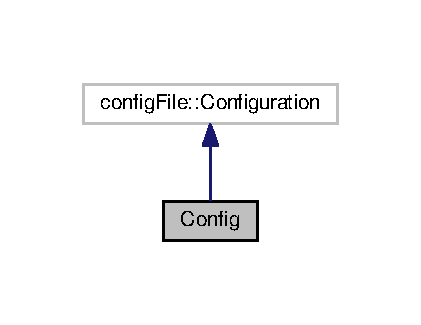
\includegraphics[width=202pt]{classConfig__inherit__graph}
\end{center}
\end{figure}


Collaboration diagram for Config\+:\nopagebreak
\begin{figure}[H]
\begin{center}
\leavevmode
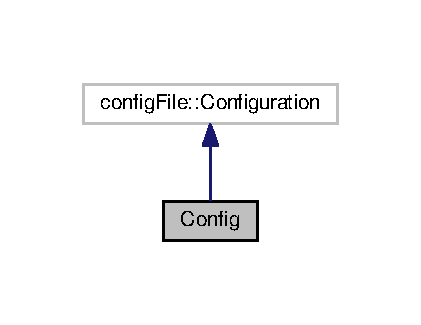
\includegraphics[width=202pt]{classConfig__coll__graph}
\end{center}
\end{figure}
\subsection*{Static Public Member Functions}
\begin{DoxyCompactItemize}
\item 
static \hyperlink{classConfig}{Config} \& \hyperlink{classConfig_a99f1af361fec85ff2071651b57377942}{get\+Instance} (std\+::string filename=\char`\"{}server.\+ini\char`\"{})
\item 
static std\+::string \hyperlink{classConfig_a54889e44629eb475653752a76e2a514e}{prettify} (std\+::string)
\end{DoxyCompactItemize}


\subsection{Member Function Documentation}
\index{Config@{Config}!get\+Instance@{get\+Instance}}
\index{get\+Instance@{get\+Instance}!Config@{Config}}
\subsubsection[{\texorpdfstring{get\+Instance(std\+::string filename=""server.\+ini"")}{getInstance(std::string filename="server.ini")}}]{\setlength{\rightskip}{0pt plus 5cm}{\bf Config} \& Config\+::get\+Instance (
\begin{DoxyParamCaption}
\item[{std\+::string}]{filename = {\ttfamily \char`\"{}server.ini\char`\"{}}}
\end{DoxyParamCaption}
)\hspace{0.3cm}{\ttfamily [static]}}\hypertarget{classConfig_a99f1af361fec85ff2071651b57377942}{}\label{classConfig_a99f1af361fec85ff2071651b57377942}
\index{Config@{Config}!prettify@{prettify}}
\index{prettify@{prettify}!Config@{Config}}
\subsubsection[{\texorpdfstring{prettify(std\+::string)}{prettify(std::string)}}]{\setlength{\rightskip}{0pt plus 5cm}std\+::string Config\+::prettify (
\begin{DoxyParamCaption}
\item[{std\+::string}]{data}
\end{DoxyParamCaption}
)\hspace{0.3cm}{\ttfamily [static]}}\hypertarget{classConfig_a54889e44629eb475653752a76e2a514e}{}\label{classConfig_a54889e44629eb475653752a76e2a514e}


The documentation for this class was generated from the following files\+:\begin{DoxyCompactItemize}
\item 
\hyperlink{config_8h}{config.\+h}\item 
\hyperlink{config_8cpp}{config.\+cpp}\end{DoxyCompactItemize}

\hypertarget{classCore_1_1IDatabase}{}\section{Core\+:\+:I\+Database Class Reference}
\label{classCore_1_1IDatabase}\index{Core\+::\+I\+Database@{Core\+::\+I\+Database}}


{\ttfamily \#include $<$core/include/idatabase.\+h$>$}



Inheritance diagram for Core\+:\+:I\+Database\+:\nopagebreak
\begin{figure}[H]
\begin{center}
\leavevmode
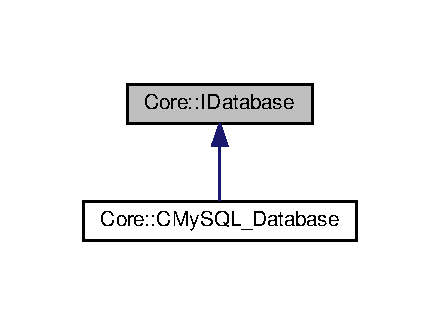
\includegraphics[width=211pt]{classCore_1_1IDatabase__inherit__graph}
\end{center}
\end{figure}
\subsection*{Public Member Functions}
\begin{DoxyCompactItemize}
\item 
virtual \hyperlink{classCore_1_1IDatabase_a81a3968a3ae51cc872cd3ce528b18da5}{$\sim$\+I\+Database} ()
\item 
virtual void \hyperlink{classCore_1_1IDatabase_ae44631affbe063b1874a24d8c5bfa7a1}{Connect} (std\+::string \+\_\+host, std\+::string \+\_\+database, std\+::string \+\_\+user, std\+::string \+\_\+password)=0
\item 
virtual void \hyperlink{classCore_1_1IDatabase_a4c99cdc857e6177f6dcbb20ec4991885}{Q\+Execute} (std\+::string \+\_\+query)=0
\item 
virtual std\+::unique\+\_\+ptr$<$ \hyperlink{classCore_1_1IResult}{I\+Result} $>$ \hyperlink{classCore_1_1IDatabase_aef93e70d32f2604712bf6439511f3485}{Q\+Store} (std\+::string \+\_\+query)=0
\end{DoxyCompactItemize}


\subsection{Constructor \& Destructor Documentation}
\index{Core\+::\+I\+Database@{Core\+::\+I\+Database}!````~I\+Database@{$\sim$\+I\+Database}}
\index{````~I\+Database@{$\sim$\+I\+Database}!Core\+::\+I\+Database@{Core\+::\+I\+Database}}
\subsubsection[{\texorpdfstring{$\sim$\+I\+Database()}{~IDatabase()}}]{\setlength{\rightskip}{0pt plus 5cm}virtual Core\+::\+I\+Database\+::$\sim$\+I\+Database (
\begin{DoxyParamCaption}
{}
\end{DoxyParamCaption}
)\hspace{0.3cm}{\ttfamily [inline]}, {\ttfamily [virtual]}}\hypertarget{classCore_1_1IDatabase_a81a3968a3ae51cc872cd3ce528b18da5}{}\label{classCore_1_1IDatabase_a81a3968a3ae51cc872cd3ce528b18da5}


\subsection{Member Function Documentation}
\index{Core\+::\+I\+Database@{Core\+::\+I\+Database}!Connect@{Connect}}
\index{Connect@{Connect}!Core\+::\+I\+Database@{Core\+::\+I\+Database}}
\subsubsection[{\texorpdfstring{Connect(std\+::string \+\_\+host, std\+::string \+\_\+database, std\+::string \+\_\+user, std\+::string \+\_\+password)=0}{Connect(std::string _host, std::string _database, std::string _user, std::string _password)=0}}]{\setlength{\rightskip}{0pt plus 5cm}virtual void Core\+::\+I\+Database\+::\+Connect (
\begin{DoxyParamCaption}
\item[{std\+::string}]{\+\_\+host, }
\item[{std\+::string}]{\+\_\+database, }
\item[{std\+::string}]{\+\_\+user, }
\item[{std\+::string}]{\+\_\+password}
\end{DoxyParamCaption}
)\hspace{0.3cm}{\ttfamily [pure virtual]}}\hypertarget{classCore_1_1IDatabase_ae44631affbe063b1874a24d8c5bfa7a1}{}\label{classCore_1_1IDatabase_ae44631affbe063b1874a24d8c5bfa7a1}


Implemented in \hyperlink{classCore_1_1CMySQL__Database_a4dd288c35b1606b4ae105b968e0f9e9d}{Core\+::\+C\+My\+S\+Q\+L\+\_\+\+Database}.

\index{Core\+::\+I\+Database@{Core\+::\+I\+Database}!Q\+Execute@{Q\+Execute}}
\index{Q\+Execute@{Q\+Execute}!Core\+::\+I\+Database@{Core\+::\+I\+Database}}
\subsubsection[{\texorpdfstring{Q\+Execute(std\+::string \+\_\+query)=0}{QExecute(std::string _query)=0}}]{\setlength{\rightskip}{0pt plus 5cm}virtual void Core\+::\+I\+Database\+::\+Q\+Execute (
\begin{DoxyParamCaption}
\item[{std\+::string}]{\+\_\+query}
\end{DoxyParamCaption}
)\hspace{0.3cm}{\ttfamily [pure virtual]}}\hypertarget{classCore_1_1IDatabase_a4c99cdc857e6177f6dcbb20ec4991885}{}\label{classCore_1_1IDatabase_a4c99cdc857e6177f6dcbb20ec4991885}


Implemented in \hyperlink{classCore_1_1CMySQL__Database_a1341fb3ef4974c6f4990334e409cd472}{Core\+::\+C\+My\+S\+Q\+L\+\_\+\+Database}.

\index{Core\+::\+I\+Database@{Core\+::\+I\+Database}!Q\+Store@{Q\+Store}}
\index{Q\+Store@{Q\+Store}!Core\+::\+I\+Database@{Core\+::\+I\+Database}}
\subsubsection[{\texorpdfstring{Q\+Store(std\+::string \+\_\+query)=0}{QStore(std::string _query)=0}}]{\setlength{\rightskip}{0pt plus 5cm}virtual std\+::unique\+\_\+ptr$<${\bf I\+Result}$>$ Core\+::\+I\+Database\+::\+Q\+Store (
\begin{DoxyParamCaption}
\item[{std\+::string}]{\+\_\+query}
\end{DoxyParamCaption}
)\hspace{0.3cm}{\ttfamily [pure virtual]}}\hypertarget{classCore_1_1IDatabase_aef93e70d32f2604712bf6439511f3485}{}\label{classCore_1_1IDatabase_aef93e70d32f2604712bf6439511f3485}


Implemented in \hyperlink{classCore_1_1CMySQL__Database_ab6b2e371bfde191cb00f98d29434e256}{Core\+::\+C\+My\+S\+Q\+L\+\_\+\+Database}.



The documentation for this class was generated from the following file\+:\begin{DoxyCompactItemize}
\item 
\hyperlink{idatabase_8h}{idatabase.\+h}\end{DoxyCompactItemize}

\hypertarget{classINetwork}{}\section{I\+Network Class Reference}
\label{classINetwork}\index{I\+Network@{I\+Network}}


{\ttfamily \#include $<$core/include/inetwork.\+h$>$}



Inheritance diagram for I\+Network\+:\nopagebreak
\begin{figure}[H]
\begin{center}
\leavevmode
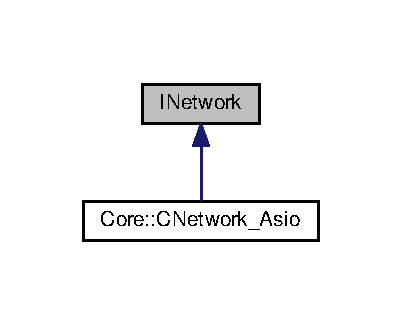
\includegraphics[width=193pt]{classINetwork__inherit__graph}
\end{center}
\end{figure}
\subsection*{Public Member Functions}
\begin{DoxyCompactItemize}
\item 
\hyperlink{classINetwork_a6c421d6cd9b2fd2662c21440d7fc275b}{I\+Network} ()
\item 
virtual \hyperlink{classINetwork_a99a59b99873361fe46ef8e97f6cd3866}{$\sim$\+I\+Network} ()
\item 
virtual bool \hyperlink{classINetwork_aff192e3d6708cb1aadef3f6667e02708}{Init} (std\+::string \+\_\+ip, uint16\+\_\+t \+\_\+port)=0
\item 
virtual bool \hyperlink{classINetwork_a6b3892964c456b4b16c8579f8833e93f}{Shutdown} ()=0
\item 
virtual bool \hyperlink{classINetwork_a1b646635942e454f2f2d938bc1fb8685}{Connect} ()=0
\item 
virtual bool \hyperlink{classINetwork_a3f47952a34fec9118c26901783009ac1}{Listen} ()=0
\item 
virtual bool \hyperlink{classINetwork_a3bfb80fcd053977e3674a2da6601f2c1}{Reconnect} ()=0
\item 
virtual bool \hyperlink{classINetwork_a44726fff2e6720f61aa34e4a4ef4780d}{Disconnect} ()=0
\item 
virtual void \hyperlink{classINetwork_a33de9938ac3a014817051b8ee626c5ff}{Set\+Id} (uint32\+\_\+t \+\_\+val)
\item 
virtual void \hyperlink{classINetwork_a1e0be185caf75e5347a2ccbce697f5e0}{Set\+Type} (uint32\+\_\+t \+\_\+val)
\item 
virtual uint32\+\_\+t \hyperlink{classINetwork_a9f2c9f0eae63deff0a01832b61337f0a}{Get\+Id} ()
\item 
virtual uint32\+\_\+t \hyperlink{classINetwork_a61ddaadedc120576b47f8b95ac02f479}{Get\+Type} ()
\item 
virtual uint16\+\_\+t \hyperlink{classINetwork_a85f9906ca9c4c94aa7a0fbe8c385c90d}{Get\+Port} ()
\item 
virtual std\+::string \hyperlink{classINetwork_a6263aaa99202ea1db4c1f939502b8dc0}{Get\+Ip\+Address} ()
\end{DoxyCompactItemize}
\subsection*{Protected Member Functions}
\begin{DoxyCompactItemize}
\item 
virtual bool \hyperlink{classINetwork_ab7738d2dffb9aad6260fca88c0c84e38}{Send} (std\+::unique\+\_\+ptr$<$ uint8\+\_\+t $>$ \+\_\+buffer)=0
\item 
virtual bool \hyperlink{classINetwork_aff58817dbf43572dff6784187e1dc128}{Recv} (uint16\+\_\+t \+\_\+size=6)=0
\item 
virtual bool \hyperlink{classINetwork_a98765191b21294b10ef55b164fccba68}{On\+Connect} ()=0
\item 
virtual void \hyperlink{classINetwork_ad5ed4b018281bf80253c62fb85c2a4b0}{On\+Connected} ()=0
\item 
virtual bool \hyperlink{classINetwork_af584043f1045c9da0eb6c21ebf1a29df}{On\+Listen} ()=0
\item 
virtual void \hyperlink{classINetwork_a5d65c0819ad2fadb745319d1d16a6f3d}{On\+Listening} ()=0
\item 
virtual bool \hyperlink{classINetwork_af73c81a512e929292a17ac4e513278e0}{On\+Disconnect} ()=0
\item 
virtual void \hyperlink{classINetwork_ad2157eb3fcf7e65a272ab5bb21791c68}{On\+Disconnected} ()=0
\item 
virtual bool \hyperlink{classINetwork_a7c7d806e714b1b2864e4841af5bb744c}{On\+Receive} ()=0
\item 
virtual bool \hyperlink{classINetwork_af9f74cbe26deddffebde1943c3969086}{On\+Received} ()=0
\item 
virtual bool \hyperlink{classINetwork_a327d045f1e37d2996c121eb7b09b59a0}{On\+Send} (uint8\+\_\+t $\ast$\+\_\+buffer)=0
\item 
virtual void \hyperlink{classINetwork_a863af3061bc113972f0c0fbfd48d15b4}{On\+Sent} ()=0
\end{DoxyCompactItemize}
\subsection*{Protected Attributes}
\begin{DoxyCompactItemize}
\item 
uint32\+\_\+t \hyperlink{classINetwork_a4c919a79e61e5b2ea107ffbe5da64edb}{network\+\_\+id\+\_\+}
\item 
uint32\+\_\+t \hyperlink{classINetwork_ac427f5a6bf1e2b9b375c12d839d4f11f}{network\+\_\+type\+\_\+}
\item 
uint16\+\_\+t \hyperlink{classINetwork_adde67598162e5b350454a49c9136c500}{network\+\_\+port\+\_\+}
\item 
std\+::string \hyperlink{classINetwork_a17f3c5cfeede0a839162320cb0bdd042}{network\+\_\+ip\+\_\+address}
\end{DoxyCompactItemize}


\subsection{Constructor \& Destructor Documentation}
\index{I\+Network@{I\+Network}!I\+Network@{I\+Network}}
\index{I\+Network@{I\+Network}!I\+Network@{I\+Network}}
\subsubsection[{\texorpdfstring{I\+Network()}{INetwork()}}]{\setlength{\rightskip}{0pt plus 5cm}I\+Network\+::\+I\+Network (
\begin{DoxyParamCaption}
{}
\end{DoxyParamCaption}
)\hspace{0.3cm}{\ttfamily [inline]}}\hypertarget{classINetwork_a6c421d6cd9b2fd2662c21440d7fc275b}{}\label{classINetwork_a6c421d6cd9b2fd2662c21440d7fc275b}
\index{I\+Network@{I\+Network}!````~I\+Network@{$\sim$\+I\+Network}}
\index{````~I\+Network@{$\sim$\+I\+Network}!I\+Network@{I\+Network}}
\subsubsection[{\texorpdfstring{$\sim$\+I\+Network()}{~INetwork()}}]{\setlength{\rightskip}{0pt plus 5cm}virtual I\+Network\+::$\sim$\+I\+Network (
\begin{DoxyParamCaption}
{}
\end{DoxyParamCaption}
)\hspace{0.3cm}{\ttfamily [inline]}, {\ttfamily [virtual]}}\hypertarget{classINetwork_a99a59b99873361fe46ef8e97f6cd3866}{}\label{classINetwork_a99a59b99873361fe46ef8e97f6cd3866}


\subsection{Member Function Documentation}
\index{I\+Network@{I\+Network}!Connect@{Connect}}
\index{Connect@{Connect}!I\+Network@{I\+Network}}
\subsubsection[{\texorpdfstring{Connect()=0}{Connect()=0}}]{\setlength{\rightskip}{0pt plus 5cm}virtual bool I\+Network\+::\+Connect (
\begin{DoxyParamCaption}
{}
\end{DoxyParamCaption}
)\hspace{0.3cm}{\ttfamily [pure virtual]}}\hypertarget{classINetwork_a1b646635942e454f2f2d938bc1fb8685}{}\label{classINetwork_a1b646635942e454f2f2d938bc1fb8685}


Implemented in \hyperlink{classCore_1_1CNetwork__Asio_a126de0c3a03d6f2efe21f2b1888285b4}{Core\+::\+C\+Network\+\_\+\+Asio}.

\index{I\+Network@{I\+Network}!Disconnect@{Disconnect}}
\index{Disconnect@{Disconnect}!I\+Network@{I\+Network}}
\subsubsection[{\texorpdfstring{Disconnect()=0}{Disconnect()=0}}]{\setlength{\rightskip}{0pt plus 5cm}virtual bool I\+Network\+::\+Disconnect (
\begin{DoxyParamCaption}
{}
\end{DoxyParamCaption}
)\hspace{0.3cm}{\ttfamily [pure virtual]}}\hypertarget{classINetwork_a44726fff2e6720f61aa34e4a4ef4780d}{}\label{classINetwork_a44726fff2e6720f61aa34e4a4ef4780d}


Implemented in \hyperlink{classCore_1_1CNetwork__Asio_aa98b86ad1ade6a4de084577a30b6d6d4}{Core\+::\+C\+Network\+\_\+\+Asio}.

\index{I\+Network@{I\+Network}!Get\+Id@{Get\+Id}}
\index{Get\+Id@{Get\+Id}!I\+Network@{I\+Network}}
\subsubsection[{\texorpdfstring{Get\+Id()}{GetId()}}]{\setlength{\rightskip}{0pt plus 5cm}virtual uint32\+\_\+t I\+Network\+::\+Get\+Id (
\begin{DoxyParamCaption}
{}
\end{DoxyParamCaption}
)\hspace{0.3cm}{\ttfamily [inline]}, {\ttfamily [virtual]}}\hypertarget{classINetwork_a9f2c9f0eae63deff0a01832b61337f0a}{}\label{classINetwork_a9f2c9f0eae63deff0a01832b61337f0a}
\index{I\+Network@{I\+Network}!Get\+Ip\+Address@{Get\+Ip\+Address}}
\index{Get\+Ip\+Address@{Get\+Ip\+Address}!I\+Network@{I\+Network}}
\subsubsection[{\texorpdfstring{Get\+Ip\+Address()}{GetIpAddress()}}]{\setlength{\rightskip}{0pt plus 5cm}virtual std\+::string I\+Network\+::\+Get\+Ip\+Address (
\begin{DoxyParamCaption}
{}
\end{DoxyParamCaption}
)\hspace{0.3cm}{\ttfamily [inline]}, {\ttfamily [virtual]}}\hypertarget{classINetwork_a6263aaa99202ea1db4c1f939502b8dc0}{}\label{classINetwork_a6263aaa99202ea1db4c1f939502b8dc0}
\index{I\+Network@{I\+Network}!Get\+Port@{Get\+Port}}
\index{Get\+Port@{Get\+Port}!I\+Network@{I\+Network}}
\subsubsection[{\texorpdfstring{Get\+Port()}{GetPort()}}]{\setlength{\rightskip}{0pt plus 5cm}virtual uint16\+\_\+t I\+Network\+::\+Get\+Port (
\begin{DoxyParamCaption}
{}
\end{DoxyParamCaption}
)\hspace{0.3cm}{\ttfamily [inline]}, {\ttfamily [virtual]}}\hypertarget{classINetwork_a85f9906ca9c4c94aa7a0fbe8c385c90d}{}\label{classINetwork_a85f9906ca9c4c94aa7a0fbe8c385c90d}
\index{I\+Network@{I\+Network}!Get\+Type@{Get\+Type}}
\index{Get\+Type@{Get\+Type}!I\+Network@{I\+Network}}
\subsubsection[{\texorpdfstring{Get\+Type()}{GetType()}}]{\setlength{\rightskip}{0pt plus 5cm}virtual uint32\+\_\+t I\+Network\+::\+Get\+Type (
\begin{DoxyParamCaption}
{}
\end{DoxyParamCaption}
)\hspace{0.3cm}{\ttfamily [inline]}, {\ttfamily [virtual]}}\hypertarget{classINetwork_a61ddaadedc120576b47f8b95ac02f479}{}\label{classINetwork_a61ddaadedc120576b47f8b95ac02f479}
\index{I\+Network@{I\+Network}!Init@{Init}}
\index{Init@{Init}!I\+Network@{I\+Network}}
\subsubsection[{\texorpdfstring{Init(std\+::string \+\_\+ip, uint16\+\_\+t \+\_\+port)=0}{Init(std::string _ip, uint16_t _port)=0}}]{\setlength{\rightskip}{0pt plus 5cm}virtual bool I\+Network\+::\+Init (
\begin{DoxyParamCaption}
\item[{std\+::string}]{\+\_\+ip, }
\item[{uint16\+\_\+t}]{\+\_\+port}
\end{DoxyParamCaption}
)\hspace{0.3cm}{\ttfamily [pure virtual]}}\hypertarget{classINetwork_aff192e3d6708cb1aadef3f6667e02708}{}\label{classINetwork_aff192e3d6708cb1aadef3f6667e02708}


Implemented in \hyperlink{classCore_1_1CNetwork__Asio_a6510dd6c07d2de995242f9ea827b97d1}{Core\+::\+C\+Network\+\_\+\+Asio}.

\index{I\+Network@{I\+Network}!Listen@{Listen}}
\index{Listen@{Listen}!I\+Network@{I\+Network}}
\subsubsection[{\texorpdfstring{Listen()=0}{Listen()=0}}]{\setlength{\rightskip}{0pt plus 5cm}virtual bool I\+Network\+::\+Listen (
\begin{DoxyParamCaption}
{}
\end{DoxyParamCaption}
)\hspace{0.3cm}{\ttfamily [pure virtual]}}\hypertarget{classINetwork_a3f47952a34fec9118c26901783009ac1}{}\label{classINetwork_a3f47952a34fec9118c26901783009ac1}


Implemented in \hyperlink{classCore_1_1CNetwork__Asio_accbfdbf25e902928bbe3809307510505}{Core\+::\+C\+Network\+\_\+\+Asio}.

\index{I\+Network@{I\+Network}!On\+Connect@{On\+Connect}}
\index{On\+Connect@{On\+Connect}!I\+Network@{I\+Network}}
\subsubsection[{\texorpdfstring{On\+Connect()=0}{OnConnect()=0}}]{\setlength{\rightskip}{0pt plus 5cm}virtual bool I\+Network\+::\+On\+Connect (
\begin{DoxyParamCaption}
{}
\end{DoxyParamCaption}
)\hspace{0.3cm}{\ttfamily [protected]}, {\ttfamily [pure virtual]}}\hypertarget{classINetwork_a98765191b21294b10ef55b164fccba68}{}\label{classINetwork_a98765191b21294b10ef55b164fccba68}


Implemented in \hyperlink{classCore_1_1CNetwork__Asio_a8b5610d420eaa22aafa429fe9d7590a9}{Core\+::\+C\+Network\+\_\+\+Asio}.

\index{I\+Network@{I\+Network}!On\+Connected@{On\+Connected}}
\index{On\+Connected@{On\+Connected}!I\+Network@{I\+Network}}
\subsubsection[{\texorpdfstring{On\+Connected()=0}{OnConnected()=0}}]{\setlength{\rightskip}{0pt plus 5cm}virtual void I\+Network\+::\+On\+Connected (
\begin{DoxyParamCaption}
{}
\end{DoxyParamCaption}
)\hspace{0.3cm}{\ttfamily [protected]}, {\ttfamily [pure virtual]}}\hypertarget{classINetwork_ad5ed4b018281bf80253c62fb85c2a4b0}{}\label{classINetwork_ad5ed4b018281bf80253c62fb85c2a4b0}


Implemented in \hyperlink{classCore_1_1CNetwork__Asio_a654726debc63f13a31e8f3c0d517259e}{Core\+::\+C\+Network\+\_\+\+Asio}.

\index{I\+Network@{I\+Network}!On\+Disconnect@{On\+Disconnect}}
\index{On\+Disconnect@{On\+Disconnect}!I\+Network@{I\+Network}}
\subsubsection[{\texorpdfstring{On\+Disconnect()=0}{OnDisconnect()=0}}]{\setlength{\rightskip}{0pt plus 5cm}virtual bool I\+Network\+::\+On\+Disconnect (
\begin{DoxyParamCaption}
{}
\end{DoxyParamCaption}
)\hspace{0.3cm}{\ttfamily [protected]}, {\ttfamily [pure virtual]}}\hypertarget{classINetwork_af73c81a512e929292a17ac4e513278e0}{}\label{classINetwork_af73c81a512e929292a17ac4e513278e0}


Implemented in \hyperlink{classCore_1_1CNetwork__Asio_afb65283ace223c5a3bea6029b8c6a809}{Core\+::\+C\+Network\+\_\+\+Asio}.

\index{I\+Network@{I\+Network}!On\+Disconnected@{On\+Disconnected}}
\index{On\+Disconnected@{On\+Disconnected}!I\+Network@{I\+Network}}
\subsubsection[{\texorpdfstring{On\+Disconnected()=0}{OnDisconnected()=0}}]{\setlength{\rightskip}{0pt plus 5cm}virtual void I\+Network\+::\+On\+Disconnected (
\begin{DoxyParamCaption}
{}
\end{DoxyParamCaption}
)\hspace{0.3cm}{\ttfamily [protected]}, {\ttfamily [pure virtual]}}\hypertarget{classINetwork_ad2157eb3fcf7e65a272ab5bb21791c68}{}\label{classINetwork_ad2157eb3fcf7e65a272ab5bb21791c68}


Implemented in \hyperlink{classCore_1_1CNetwork__Asio_a1e813736a887fe3a128b1672be1cbb10}{Core\+::\+C\+Network\+\_\+\+Asio}.

\index{I\+Network@{I\+Network}!On\+Listen@{On\+Listen}}
\index{On\+Listen@{On\+Listen}!I\+Network@{I\+Network}}
\subsubsection[{\texorpdfstring{On\+Listen()=0}{OnListen()=0}}]{\setlength{\rightskip}{0pt plus 5cm}virtual bool I\+Network\+::\+On\+Listen (
\begin{DoxyParamCaption}
{}
\end{DoxyParamCaption}
)\hspace{0.3cm}{\ttfamily [protected]}, {\ttfamily [pure virtual]}}\hypertarget{classINetwork_af584043f1045c9da0eb6c21ebf1a29df}{}\label{classINetwork_af584043f1045c9da0eb6c21ebf1a29df}


Implemented in \hyperlink{classCore_1_1CNetwork__Asio_a09c413ff854b8d8aa53b09f3eb610a34}{Core\+::\+C\+Network\+\_\+\+Asio}.

\index{I\+Network@{I\+Network}!On\+Listening@{On\+Listening}}
\index{On\+Listening@{On\+Listening}!I\+Network@{I\+Network}}
\subsubsection[{\texorpdfstring{On\+Listening()=0}{OnListening()=0}}]{\setlength{\rightskip}{0pt plus 5cm}virtual void I\+Network\+::\+On\+Listening (
\begin{DoxyParamCaption}
{}
\end{DoxyParamCaption}
)\hspace{0.3cm}{\ttfamily [protected]}, {\ttfamily [pure virtual]}}\hypertarget{classINetwork_a5d65c0819ad2fadb745319d1d16a6f3d}{}\label{classINetwork_a5d65c0819ad2fadb745319d1d16a6f3d}


Implemented in \hyperlink{classCore_1_1CNetwork__Asio_a1534e01f0aae39a12af3ac3e88aa7954}{Core\+::\+C\+Network\+\_\+\+Asio}.

\index{I\+Network@{I\+Network}!On\+Receive@{On\+Receive}}
\index{On\+Receive@{On\+Receive}!I\+Network@{I\+Network}}
\subsubsection[{\texorpdfstring{On\+Receive()=0}{OnReceive()=0}}]{\setlength{\rightskip}{0pt plus 5cm}virtual bool I\+Network\+::\+On\+Receive (
\begin{DoxyParamCaption}
{}
\end{DoxyParamCaption}
)\hspace{0.3cm}{\ttfamily [protected]}, {\ttfamily [pure virtual]}}\hypertarget{classINetwork_a7c7d806e714b1b2864e4841af5bb744c}{}\label{classINetwork_a7c7d806e714b1b2864e4841af5bb744c}


Implemented in \hyperlink{classCore_1_1CNetwork__Asio_af97c853ab0bcba0372919f0a243f4cb5}{Core\+::\+C\+Network\+\_\+\+Asio}.

\index{I\+Network@{I\+Network}!On\+Received@{On\+Received}}
\index{On\+Received@{On\+Received}!I\+Network@{I\+Network}}
\subsubsection[{\texorpdfstring{On\+Received()=0}{OnReceived()=0}}]{\setlength{\rightskip}{0pt plus 5cm}virtual bool I\+Network\+::\+On\+Received (
\begin{DoxyParamCaption}
{}
\end{DoxyParamCaption}
)\hspace{0.3cm}{\ttfamily [protected]}, {\ttfamily [pure virtual]}}\hypertarget{classINetwork_af9f74cbe26deddffebde1943c3969086}{}\label{classINetwork_af9f74cbe26deddffebde1943c3969086}


Implemented in \hyperlink{classCore_1_1CNetwork__Asio_acb2952682b6abbce60b01d9c75b02729}{Core\+::\+C\+Network\+\_\+\+Asio}.

\index{I\+Network@{I\+Network}!On\+Send@{On\+Send}}
\index{On\+Send@{On\+Send}!I\+Network@{I\+Network}}
\subsubsection[{\texorpdfstring{On\+Send(uint8\+\_\+t $\ast$\+\_\+buffer)=0}{OnSend(uint8_t *_buffer)=0}}]{\setlength{\rightskip}{0pt plus 5cm}virtual bool I\+Network\+::\+On\+Send (
\begin{DoxyParamCaption}
\item[{uint8\+\_\+t $\ast$}]{\+\_\+buffer}
\end{DoxyParamCaption}
)\hspace{0.3cm}{\ttfamily [protected]}, {\ttfamily [pure virtual]}}\hypertarget{classINetwork_a327d045f1e37d2996c121eb7b09b59a0}{}\label{classINetwork_a327d045f1e37d2996c121eb7b09b59a0}


Implemented in \hyperlink{classCore_1_1CNetwork__Asio_a3cfea157222e7ef2c1e67f2c0e25ed8c}{Core\+::\+C\+Network\+\_\+\+Asio}.

\index{I\+Network@{I\+Network}!On\+Sent@{On\+Sent}}
\index{On\+Sent@{On\+Sent}!I\+Network@{I\+Network}}
\subsubsection[{\texorpdfstring{On\+Sent()=0}{OnSent()=0}}]{\setlength{\rightskip}{0pt plus 5cm}virtual void I\+Network\+::\+On\+Sent (
\begin{DoxyParamCaption}
{}
\end{DoxyParamCaption}
)\hspace{0.3cm}{\ttfamily [protected]}, {\ttfamily [pure virtual]}}\hypertarget{classINetwork_a863af3061bc113972f0c0fbfd48d15b4}{}\label{classINetwork_a863af3061bc113972f0c0fbfd48d15b4}


Implemented in \hyperlink{classCore_1_1CNetwork__Asio_a79ff0fbfb787e26a079ef259160de6e3}{Core\+::\+C\+Network\+\_\+\+Asio}.

\index{I\+Network@{I\+Network}!Reconnect@{Reconnect}}
\index{Reconnect@{Reconnect}!I\+Network@{I\+Network}}
\subsubsection[{\texorpdfstring{Reconnect()=0}{Reconnect()=0}}]{\setlength{\rightskip}{0pt plus 5cm}virtual bool I\+Network\+::\+Reconnect (
\begin{DoxyParamCaption}
{}
\end{DoxyParamCaption}
)\hspace{0.3cm}{\ttfamily [pure virtual]}}\hypertarget{classINetwork_a3bfb80fcd053977e3674a2da6601f2c1}{}\label{classINetwork_a3bfb80fcd053977e3674a2da6601f2c1}


Implemented in \hyperlink{classCore_1_1CNetwork__Asio_a57f1ef8e8849990b393b27fcece6871d}{Core\+::\+C\+Network\+\_\+\+Asio}.

\index{I\+Network@{I\+Network}!Recv@{Recv}}
\index{Recv@{Recv}!I\+Network@{I\+Network}}
\subsubsection[{\texorpdfstring{Recv(uint16\+\_\+t \+\_\+size=6)=0}{Recv(uint16_t _size=6)=0}}]{\setlength{\rightskip}{0pt plus 5cm}virtual bool I\+Network\+::\+Recv (
\begin{DoxyParamCaption}
\item[{uint16\+\_\+t}]{\+\_\+size = {\ttfamily 6}}
\end{DoxyParamCaption}
)\hspace{0.3cm}{\ttfamily [protected]}, {\ttfamily [pure virtual]}}\hypertarget{classINetwork_aff58817dbf43572dff6784187e1dc128}{}\label{classINetwork_aff58817dbf43572dff6784187e1dc128}


Implemented in \hyperlink{classCore_1_1CNetwork__Asio_a08865b2606dcef0e38f27532b1ae3909}{Core\+::\+C\+Network\+\_\+\+Asio}.

\index{I\+Network@{I\+Network}!Send@{Send}}
\index{Send@{Send}!I\+Network@{I\+Network}}
\subsubsection[{\texorpdfstring{Send(std\+::unique\+\_\+ptr$<$ uint8\+\_\+t $>$ \+\_\+buffer)=0}{Send(std::unique_ptr< uint8_t > _buffer)=0}}]{\setlength{\rightskip}{0pt plus 5cm}virtual bool I\+Network\+::\+Send (
\begin{DoxyParamCaption}
\item[{std\+::unique\+\_\+ptr$<$ uint8\+\_\+t $>$}]{\+\_\+buffer}
\end{DoxyParamCaption}
)\hspace{0.3cm}{\ttfamily [protected]}, {\ttfamily [pure virtual]}}\hypertarget{classINetwork_ab7738d2dffb9aad6260fca88c0c84e38}{}\label{classINetwork_ab7738d2dffb9aad6260fca88c0c84e38}


Implemented in \hyperlink{classCore_1_1CNetwork__Asio_a2f84428ff2250e960ba2739b45f491a2}{Core\+::\+C\+Network\+\_\+\+Asio}.

\index{I\+Network@{I\+Network}!Set\+Id@{Set\+Id}}
\index{Set\+Id@{Set\+Id}!I\+Network@{I\+Network}}
\subsubsection[{\texorpdfstring{Set\+Id(uint32\+\_\+t \+\_\+val)}{SetId(uint32_t _val)}}]{\setlength{\rightskip}{0pt plus 5cm}virtual void I\+Network\+::\+Set\+Id (
\begin{DoxyParamCaption}
\item[{uint32\+\_\+t}]{\+\_\+val}
\end{DoxyParamCaption}
)\hspace{0.3cm}{\ttfamily [inline]}, {\ttfamily [virtual]}}\hypertarget{classINetwork_a33de9938ac3a014817051b8ee626c5ff}{}\label{classINetwork_a33de9938ac3a014817051b8ee626c5ff}
\index{I\+Network@{I\+Network}!Set\+Type@{Set\+Type}}
\index{Set\+Type@{Set\+Type}!I\+Network@{I\+Network}}
\subsubsection[{\texorpdfstring{Set\+Type(uint32\+\_\+t \+\_\+val)}{SetType(uint32_t _val)}}]{\setlength{\rightskip}{0pt plus 5cm}virtual void I\+Network\+::\+Set\+Type (
\begin{DoxyParamCaption}
\item[{uint32\+\_\+t}]{\+\_\+val}
\end{DoxyParamCaption}
)\hspace{0.3cm}{\ttfamily [inline]}, {\ttfamily [virtual]}}\hypertarget{classINetwork_a1e0be185caf75e5347a2ccbce697f5e0}{}\label{classINetwork_a1e0be185caf75e5347a2ccbce697f5e0}
\index{I\+Network@{I\+Network}!Shutdown@{Shutdown}}
\index{Shutdown@{Shutdown}!I\+Network@{I\+Network}}
\subsubsection[{\texorpdfstring{Shutdown()=0}{Shutdown()=0}}]{\setlength{\rightskip}{0pt plus 5cm}virtual bool I\+Network\+::\+Shutdown (
\begin{DoxyParamCaption}
{}
\end{DoxyParamCaption}
)\hspace{0.3cm}{\ttfamily [pure virtual]}}\hypertarget{classINetwork_a6b3892964c456b4b16c8579f8833e93f}{}\label{classINetwork_a6b3892964c456b4b16c8579f8833e93f}


Implemented in \hyperlink{classCore_1_1CNetwork__Asio_a1990de08bdc733e76d575f13b03072d0}{Core\+::\+C\+Network\+\_\+\+Asio}.



\subsection{Member Data Documentation}
\index{I\+Network@{I\+Network}!network\+\_\+id\+\_\+@{network\+\_\+id\+\_\+}}
\index{network\+\_\+id\+\_\+@{network\+\_\+id\+\_\+}!I\+Network@{I\+Network}}
\subsubsection[{\texorpdfstring{network\+\_\+id\+\_\+}{network_id_}}]{\setlength{\rightskip}{0pt plus 5cm}uint32\+\_\+t I\+Network\+::network\+\_\+id\+\_\+\hspace{0.3cm}{\ttfamily [protected]}}\hypertarget{classINetwork_a4c919a79e61e5b2ea107ffbe5da64edb}{}\label{classINetwork_a4c919a79e61e5b2ea107ffbe5da64edb}
\index{I\+Network@{I\+Network}!network\+\_\+ip\+\_\+address@{network\+\_\+ip\+\_\+address}}
\index{network\+\_\+ip\+\_\+address@{network\+\_\+ip\+\_\+address}!I\+Network@{I\+Network}}
\subsubsection[{\texorpdfstring{network\+\_\+ip\+\_\+address}{network_ip_address}}]{\setlength{\rightskip}{0pt plus 5cm}std\+::string I\+Network\+::network\+\_\+ip\+\_\+address\hspace{0.3cm}{\ttfamily [protected]}}\hypertarget{classINetwork_a17f3c5cfeede0a839162320cb0bdd042}{}\label{classINetwork_a17f3c5cfeede0a839162320cb0bdd042}
\index{I\+Network@{I\+Network}!network\+\_\+port\+\_\+@{network\+\_\+port\+\_\+}}
\index{network\+\_\+port\+\_\+@{network\+\_\+port\+\_\+}!I\+Network@{I\+Network}}
\subsubsection[{\texorpdfstring{network\+\_\+port\+\_\+}{network_port_}}]{\setlength{\rightskip}{0pt plus 5cm}uint16\+\_\+t I\+Network\+::network\+\_\+port\+\_\+\hspace{0.3cm}{\ttfamily [protected]}}\hypertarget{classINetwork_adde67598162e5b350454a49c9136c500}{}\label{classINetwork_adde67598162e5b350454a49c9136c500}
\index{I\+Network@{I\+Network}!network\+\_\+type\+\_\+@{network\+\_\+type\+\_\+}}
\index{network\+\_\+type\+\_\+@{network\+\_\+type\+\_\+}!I\+Network@{I\+Network}}
\subsubsection[{\texorpdfstring{network\+\_\+type\+\_\+}{network_type_}}]{\setlength{\rightskip}{0pt plus 5cm}uint32\+\_\+t I\+Network\+::network\+\_\+type\+\_\+\hspace{0.3cm}{\ttfamily [protected]}}\hypertarget{classINetwork_ac427f5a6bf1e2b9b375c12d839d4f11f}{}\label{classINetwork_ac427f5a6bf1e2b9b375c12d839d4f11f}


The documentation for this class was generated from the following file\+:\begin{DoxyCompactItemize}
\item 
\hyperlink{inetwork_8h}{inetwork.\+h}\end{DoxyCompactItemize}

\hypertarget{classCore_1_1IResult}{}\section{Core\+:\+:I\+Result Class Reference}
\label{classCore_1_1IResult}\index{Core\+::\+I\+Result@{Core\+::\+I\+Result}}


{\ttfamily \#include $<$core/include/idatabase.\+h$>$}



Inheritance diagram for Core\+:\+:I\+Result\+:\nopagebreak
\begin{figure}[H]
\begin{center}
\leavevmode
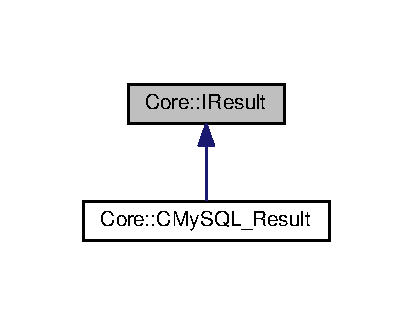
\includegraphics[width=198pt]{classCore_1_1IResult__inherit__graph}
\end{center}
\end{figure}
\subsection*{Public Types}
\begin{DoxyCompactItemize}
\item 
typedef std\+::vector$<$ std\+::unique\+\_\+ptr$<$ \hyperlink{classCore_1_1IRow}{I\+Row} $>$ $>$\+::\hyperlink{classCore_1_1IResult_a1b8d24ea97ebbe669bb13c09ad5ad796}{iterator} \hyperlink{classCore_1_1IResult_a1b8d24ea97ebbe669bb13c09ad5ad796}{iterator}
\item 
typedef std\+::vector$<$ std\+::unique\+\_\+ptr$<$ \hyperlink{classCore_1_1IRow}{I\+Row} $>$ $>$\+::\hyperlink{classCore_1_1IResult_a4f549868ef8d40c199565efd7b89f45c}{const\+\_\+iterator} \hyperlink{classCore_1_1IResult_a4f549868ef8d40c199565efd7b89f45c}{const\+\_\+iterator}
\end{DoxyCompactItemize}
\subsection*{Public Member Functions}
\begin{DoxyCompactItemize}
\item 
\hyperlink{classCore_1_1IResult_a4ef27140c899f8d161cdcd6b530ac379}{I\+Result} ()
\item 
virtual \hyperlink{classCore_1_1IResult_a73060de3740b154e3400fbbe9c5b984b}{$\sim$\+I\+Result} ()
\item 
virtual void \hyperlink{classCore_1_1IResult_ae0b4b5bca1f1ad8d4d7d887b656c67a7}{use\+Row} (uint32\+\_\+t \+\_\+row)
\item 
virtual bool \hyperlink{classCore_1_1IResult_a93fe49ee2a9ab7ed520293d9e1339a96}{increment\+Row} ()
\item 
virtual bool \hyperlink{classCore_1_1IResult_a3c210ff7fa555d104732198808356488}{decrement\+Row} ()
\item 
virtual uint32\+\_\+t \hyperlink{classCore_1_1IResult_a308ce2382287ba5de5102fc532097709}{size} () const =0
\item 
virtual bool \hyperlink{classCore_1_1IResult_a6b96b8324d81a1a65d60a4f6a6e78052}{get\+String} (std\+::string const \&column\+Name, std\+::string \&data)=0
\item 
virtual bool \hyperlink{classCore_1_1IResult_a9c01330c5b826ca948b48e13a330f4cd}{get\+Int} (std\+::string const \&column\+Name, uint32\+\_\+t \&data)=0
\item 
virtual bool \hyperlink{classCore_1_1IResult_a32e076c5c5ba522e4c58095637fe0f3e}{get\+Float} (std\+::string const \&column\+Name, float \&data)=0
\item 
virtual \hyperlink{classCore_1_1IResult_a1b8d24ea97ebbe669bb13c09ad5ad796}{iterator} \hyperlink{classCore_1_1IResult_a63b3ed4907f4735ed0bf044d3ab8dca8}{begin} ()
\item 
virtual \hyperlink{classCore_1_1IResult_a1b8d24ea97ebbe669bb13c09ad5ad796}{iterator} \hyperlink{classCore_1_1IResult_af2845d0ea33b90ea185af8904e336424}{end} ()
\item 
virtual \hyperlink{classCore_1_1IResult_a4f549868ef8d40c199565efd7b89f45c}{const\+\_\+iterator} \hyperlink{classCore_1_1IResult_a01a761f10597a834c9a26c0e58825973}{cbegin} () const 
\item 
virtual \hyperlink{classCore_1_1IResult_a4f549868ef8d40c199565efd7b89f45c}{const\+\_\+iterator} \hyperlink{classCore_1_1IResult_a73c390c4889a8ae7aaaf07e0dfd05fb4}{cend} () const 
\end{DoxyCompactItemize}
\subsection*{Protected Attributes}
\begin{DoxyCompactItemize}
\item 
uint32\+\_\+t \hyperlink{classCore_1_1IResult_a43afac5e5868af6111ae94d01ae98b28}{current\+\_\+row\+\_\+}
\item 
std\+::vector$<$ std\+::unique\+\_\+ptr$<$ \hyperlink{classCore_1_1IRow}{I\+Row} $>$ $>$ \hyperlink{classCore_1_1IResult_a80b0e69abcc0fdc6a4efa005ae81834c}{rows\+\_\+}
\end{DoxyCompactItemize}


\subsection{Member Typedef Documentation}
\index{Core\+::\+I\+Result@{Core\+::\+I\+Result}!const\+\_\+iterator@{const\+\_\+iterator}}
\index{const\+\_\+iterator@{const\+\_\+iterator}!Core\+::\+I\+Result@{Core\+::\+I\+Result}}
\subsubsection[{\texorpdfstring{const\+\_\+iterator}{const_iterator}}]{\setlength{\rightskip}{0pt plus 5cm}typedef std\+::vector$<$std\+::unique\+\_\+ptr$<${\bf I\+Row}$>$ $>$\+::{\bf const\+\_\+iterator} {\bf Core\+::\+I\+Result\+::const\+\_\+iterator}}\hypertarget{classCore_1_1IResult_a4f549868ef8d40c199565efd7b89f45c}{}\label{classCore_1_1IResult_a4f549868ef8d40c199565efd7b89f45c}
\index{Core\+::\+I\+Result@{Core\+::\+I\+Result}!iterator@{iterator}}
\index{iterator@{iterator}!Core\+::\+I\+Result@{Core\+::\+I\+Result}}
\subsubsection[{\texorpdfstring{iterator}{iterator}}]{\setlength{\rightskip}{0pt plus 5cm}typedef std\+::vector$<$std\+::unique\+\_\+ptr$<${\bf I\+Row}$>$ $>$\+::{\bf iterator} {\bf Core\+::\+I\+Result\+::iterator}}\hypertarget{classCore_1_1IResult_a1b8d24ea97ebbe669bb13c09ad5ad796}{}\label{classCore_1_1IResult_a1b8d24ea97ebbe669bb13c09ad5ad796}


\subsection{Constructor \& Destructor Documentation}
\index{Core\+::\+I\+Result@{Core\+::\+I\+Result}!I\+Result@{I\+Result}}
\index{I\+Result@{I\+Result}!Core\+::\+I\+Result@{Core\+::\+I\+Result}}
\subsubsection[{\texorpdfstring{I\+Result()}{IResult()}}]{\setlength{\rightskip}{0pt plus 5cm}Core\+::\+I\+Result\+::\+I\+Result (
\begin{DoxyParamCaption}
{}
\end{DoxyParamCaption}
)\hspace{0.3cm}{\ttfamily [inline]}}\hypertarget{classCore_1_1IResult_a4ef27140c899f8d161cdcd6b530ac379}{}\label{classCore_1_1IResult_a4ef27140c899f8d161cdcd6b530ac379}
\index{Core\+::\+I\+Result@{Core\+::\+I\+Result}!````~I\+Result@{$\sim$\+I\+Result}}
\index{````~I\+Result@{$\sim$\+I\+Result}!Core\+::\+I\+Result@{Core\+::\+I\+Result}}
\subsubsection[{\texorpdfstring{$\sim$\+I\+Result()}{~IResult()}}]{\setlength{\rightskip}{0pt plus 5cm}virtual Core\+::\+I\+Result\+::$\sim$\+I\+Result (
\begin{DoxyParamCaption}
{}
\end{DoxyParamCaption}
)\hspace{0.3cm}{\ttfamily [inline]}, {\ttfamily [virtual]}}\hypertarget{classCore_1_1IResult_a73060de3740b154e3400fbbe9c5b984b}{}\label{classCore_1_1IResult_a73060de3740b154e3400fbbe9c5b984b}


\subsection{Member Function Documentation}
\index{Core\+::\+I\+Result@{Core\+::\+I\+Result}!begin@{begin}}
\index{begin@{begin}!Core\+::\+I\+Result@{Core\+::\+I\+Result}}
\subsubsection[{\texorpdfstring{begin()}{begin()}}]{\setlength{\rightskip}{0pt plus 5cm}virtual {\bf iterator} Core\+::\+I\+Result\+::begin (
\begin{DoxyParamCaption}
{}
\end{DoxyParamCaption}
)\hspace{0.3cm}{\ttfamily [inline]}, {\ttfamily [virtual]}}\hypertarget{classCore_1_1IResult_a63b3ed4907f4735ed0bf044d3ab8dca8}{}\label{classCore_1_1IResult_a63b3ed4907f4735ed0bf044d3ab8dca8}
\index{Core\+::\+I\+Result@{Core\+::\+I\+Result}!cbegin@{cbegin}}
\index{cbegin@{cbegin}!Core\+::\+I\+Result@{Core\+::\+I\+Result}}
\subsubsection[{\texorpdfstring{cbegin() const }{cbegin() const }}]{\setlength{\rightskip}{0pt plus 5cm}virtual {\bf const\+\_\+iterator} Core\+::\+I\+Result\+::cbegin (
\begin{DoxyParamCaption}
{}
\end{DoxyParamCaption}
) const\hspace{0.3cm}{\ttfamily [inline]}, {\ttfamily [virtual]}}\hypertarget{classCore_1_1IResult_a01a761f10597a834c9a26c0e58825973}{}\label{classCore_1_1IResult_a01a761f10597a834c9a26c0e58825973}
\index{Core\+::\+I\+Result@{Core\+::\+I\+Result}!cend@{cend}}
\index{cend@{cend}!Core\+::\+I\+Result@{Core\+::\+I\+Result}}
\subsubsection[{\texorpdfstring{cend() const }{cend() const }}]{\setlength{\rightskip}{0pt plus 5cm}virtual {\bf const\+\_\+iterator} Core\+::\+I\+Result\+::cend (
\begin{DoxyParamCaption}
{}
\end{DoxyParamCaption}
) const\hspace{0.3cm}{\ttfamily [inline]}, {\ttfamily [virtual]}}\hypertarget{classCore_1_1IResult_a73c390c4889a8ae7aaaf07e0dfd05fb4}{}\label{classCore_1_1IResult_a73c390c4889a8ae7aaaf07e0dfd05fb4}
\index{Core\+::\+I\+Result@{Core\+::\+I\+Result}!decrement\+Row@{decrement\+Row}}
\index{decrement\+Row@{decrement\+Row}!Core\+::\+I\+Result@{Core\+::\+I\+Result}}
\subsubsection[{\texorpdfstring{decrement\+Row()}{decrementRow()}}]{\setlength{\rightskip}{0pt plus 5cm}virtual bool Core\+::\+I\+Result\+::decrement\+Row (
\begin{DoxyParamCaption}
{}
\end{DoxyParamCaption}
)\hspace{0.3cm}{\ttfamily [inline]}, {\ttfamily [virtual]}}\hypertarget{classCore_1_1IResult_a3c210ff7fa555d104732198808356488}{}\label{classCore_1_1IResult_a3c210ff7fa555d104732198808356488}
\index{Core\+::\+I\+Result@{Core\+::\+I\+Result}!end@{end}}
\index{end@{end}!Core\+::\+I\+Result@{Core\+::\+I\+Result}}
\subsubsection[{\texorpdfstring{end()}{end()}}]{\setlength{\rightskip}{0pt plus 5cm}virtual {\bf iterator} Core\+::\+I\+Result\+::end (
\begin{DoxyParamCaption}
{}
\end{DoxyParamCaption}
)\hspace{0.3cm}{\ttfamily [inline]}, {\ttfamily [virtual]}}\hypertarget{classCore_1_1IResult_af2845d0ea33b90ea185af8904e336424}{}\label{classCore_1_1IResult_af2845d0ea33b90ea185af8904e336424}
\index{Core\+::\+I\+Result@{Core\+::\+I\+Result}!get\+Float@{get\+Float}}
\index{get\+Float@{get\+Float}!Core\+::\+I\+Result@{Core\+::\+I\+Result}}
\subsubsection[{\texorpdfstring{get\+Float(std\+::string const \&column\+Name, float \&data)=0}{getFloat(std::string const &columnName, float &data)=0}}]{\setlength{\rightskip}{0pt plus 5cm}virtual bool Core\+::\+I\+Result\+::get\+Float (
\begin{DoxyParamCaption}
\item[{std\+::string const \&}]{column\+Name, }
\item[{float \&}]{data}
\end{DoxyParamCaption}
)\hspace{0.3cm}{\ttfamily [pure virtual]}}\hypertarget{classCore_1_1IResult_a32e076c5c5ba522e4c58095637fe0f3e}{}\label{classCore_1_1IResult_a32e076c5c5ba522e4c58095637fe0f3e}


Implemented in \hyperlink{classCore_1_1CMySQL__Result_aa3d600b73235197ae49926fdc726e1a2}{Core\+::\+C\+My\+S\+Q\+L\+\_\+\+Result}.

\index{Core\+::\+I\+Result@{Core\+::\+I\+Result}!get\+Int@{get\+Int}}
\index{get\+Int@{get\+Int}!Core\+::\+I\+Result@{Core\+::\+I\+Result}}
\subsubsection[{\texorpdfstring{get\+Int(std\+::string const \&column\+Name, uint32\+\_\+t \&data)=0}{getInt(std::string const &columnName, uint32_t &data)=0}}]{\setlength{\rightskip}{0pt plus 5cm}virtual bool Core\+::\+I\+Result\+::get\+Int (
\begin{DoxyParamCaption}
\item[{std\+::string const \&}]{column\+Name, }
\item[{uint32\+\_\+t \&}]{data}
\end{DoxyParamCaption}
)\hspace{0.3cm}{\ttfamily [pure virtual]}}\hypertarget{classCore_1_1IResult_a9c01330c5b826ca948b48e13a330f4cd}{}\label{classCore_1_1IResult_a9c01330c5b826ca948b48e13a330f4cd}


Implemented in \hyperlink{classCore_1_1CMySQL__Result_add098e59d4e53d790a8934acc64543e8}{Core\+::\+C\+My\+S\+Q\+L\+\_\+\+Result}.

\index{Core\+::\+I\+Result@{Core\+::\+I\+Result}!get\+String@{get\+String}}
\index{get\+String@{get\+String}!Core\+::\+I\+Result@{Core\+::\+I\+Result}}
\subsubsection[{\texorpdfstring{get\+String(std\+::string const \&column\+Name, std\+::string \&data)=0}{getString(std::string const &columnName, std::string &data)=0}}]{\setlength{\rightskip}{0pt plus 5cm}virtual bool Core\+::\+I\+Result\+::get\+String (
\begin{DoxyParamCaption}
\item[{std\+::string const \&}]{column\+Name, }
\item[{std\+::string \&}]{data}
\end{DoxyParamCaption}
)\hspace{0.3cm}{\ttfamily [pure virtual]}}\hypertarget{classCore_1_1IResult_a6b96b8324d81a1a65d60a4f6a6e78052}{}\label{classCore_1_1IResult_a6b96b8324d81a1a65d60a4f6a6e78052}


Implemented in \hyperlink{classCore_1_1CMySQL__Result_a839fa1572ea7a20041ec8b5181017e80}{Core\+::\+C\+My\+S\+Q\+L\+\_\+\+Result}.

\index{Core\+::\+I\+Result@{Core\+::\+I\+Result}!increment\+Row@{increment\+Row}}
\index{increment\+Row@{increment\+Row}!Core\+::\+I\+Result@{Core\+::\+I\+Result}}
\subsubsection[{\texorpdfstring{increment\+Row()}{incrementRow()}}]{\setlength{\rightskip}{0pt plus 5cm}virtual bool Core\+::\+I\+Result\+::increment\+Row (
\begin{DoxyParamCaption}
{}
\end{DoxyParamCaption}
)\hspace{0.3cm}{\ttfamily [inline]}, {\ttfamily [virtual]}}\hypertarget{classCore_1_1IResult_a93fe49ee2a9ab7ed520293d9e1339a96}{}\label{classCore_1_1IResult_a93fe49ee2a9ab7ed520293d9e1339a96}


Reimplemented in \hyperlink{classCore_1_1CMySQL__Result_a432de24b42bb64ff4eb082ee6db97d52}{Core\+::\+C\+My\+S\+Q\+L\+\_\+\+Result}.

\index{Core\+::\+I\+Result@{Core\+::\+I\+Result}!size@{size}}
\index{size@{size}!Core\+::\+I\+Result@{Core\+::\+I\+Result}}
\subsubsection[{\texorpdfstring{size() const =0}{size() const =0}}]{\setlength{\rightskip}{0pt plus 5cm}virtual uint32\+\_\+t Core\+::\+I\+Result\+::size (
\begin{DoxyParamCaption}
{}
\end{DoxyParamCaption}
) const\hspace{0.3cm}{\ttfamily [pure virtual]}}\hypertarget{classCore_1_1IResult_a308ce2382287ba5de5102fc532097709}{}\label{classCore_1_1IResult_a308ce2382287ba5de5102fc532097709}


Implemented in \hyperlink{classCore_1_1CMySQL__Result_af5e5f0783f0ee7e09ae508bb81176bb8}{Core\+::\+C\+My\+S\+Q\+L\+\_\+\+Result}.

\index{Core\+::\+I\+Result@{Core\+::\+I\+Result}!use\+Row@{use\+Row}}
\index{use\+Row@{use\+Row}!Core\+::\+I\+Result@{Core\+::\+I\+Result}}
\subsubsection[{\texorpdfstring{use\+Row(uint32\+\_\+t \+\_\+row)}{useRow(uint32_t _row)}}]{\setlength{\rightskip}{0pt plus 5cm}virtual void Core\+::\+I\+Result\+::use\+Row (
\begin{DoxyParamCaption}
\item[{uint32\+\_\+t}]{\+\_\+row}
\end{DoxyParamCaption}
)\hspace{0.3cm}{\ttfamily [inline]}, {\ttfamily [virtual]}}\hypertarget{classCore_1_1IResult_ae0b4b5bca1f1ad8d4d7d887b656c67a7}{}\label{classCore_1_1IResult_ae0b4b5bca1f1ad8d4d7d887b656c67a7}


\subsection{Member Data Documentation}
\index{Core\+::\+I\+Result@{Core\+::\+I\+Result}!current\+\_\+row\+\_\+@{current\+\_\+row\+\_\+}}
\index{current\+\_\+row\+\_\+@{current\+\_\+row\+\_\+}!Core\+::\+I\+Result@{Core\+::\+I\+Result}}
\subsubsection[{\texorpdfstring{current\+\_\+row\+\_\+}{current_row_}}]{\setlength{\rightskip}{0pt plus 5cm}uint32\+\_\+t Core\+::\+I\+Result\+::current\+\_\+row\+\_\+\hspace{0.3cm}{\ttfamily [protected]}}\hypertarget{classCore_1_1IResult_a43afac5e5868af6111ae94d01ae98b28}{}\label{classCore_1_1IResult_a43afac5e5868af6111ae94d01ae98b28}
\index{Core\+::\+I\+Result@{Core\+::\+I\+Result}!rows\+\_\+@{rows\+\_\+}}
\index{rows\+\_\+@{rows\+\_\+}!Core\+::\+I\+Result@{Core\+::\+I\+Result}}
\subsubsection[{\texorpdfstring{rows\+\_\+}{rows_}}]{\setlength{\rightskip}{0pt plus 5cm}std\+::vector$<$std\+::unique\+\_\+ptr$<${\bf I\+Row}$>$ $>$ Core\+::\+I\+Result\+::rows\+\_\+\hspace{0.3cm}{\ttfamily [protected]}}\hypertarget{classCore_1_1IResult_a80b0e69abcc0fdc6a4efa005ae81834c}{}\label{classCore_1_1IResult_a80b0e69abcc0fdc6a4efa005ae81834c}


The documentation for this class was generated from the following file\+:\begin{DoxyCompactItemize}
\item 
\hyperlink{idatabase_8h}{idatabase.\+h}\end{DoxyCompactItemize}

\hypertarget{classCore_1_1IRow}{}\section{Core\+:\+:I\+Row Class Reference}
\label{classCore_1_1IRow}\index{Core\+::\+I\+Row@{Core\+::\+I\+Row}}


{\ttfamily \#include $<$core/include/idatabase.\+h$>$}



Inheritance diagram for Core\+:\+:I\+Row\+:\nopagebreak
\begin{figure}[H]
\begin{center}
\leavevmode
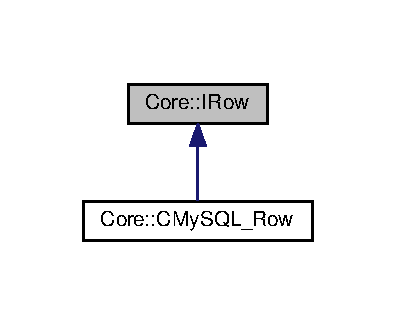
\includegraphics[width=190pt]{classCore_1_1IRow__inherit__graph}
\end{center}
\end{figure}
\subsection*{Public Member Functions}
\begin{DoxyCompactItemize}
\item 
virtual \hyperlink{classCore_1_1IRow_ade25e85bd222d88d9a1fd7899a90ad85}{$\sim$\+I\+Row} ()
\item 
virtual bool \hyperlink{classCore_1_1IRow_a6237dc736cc99b00880ef0d8df2544ff}{get\+String} (std\+::string const \&column\+Name, std\+::string \&data)=0
\item 
virtual bool \hyperlink{classCore_1_1IRow_aa90ad0d42f61cc3101b8b13b389eb5b3}{get\+Int} (std\+::string const \&column\+Name, uint32\+\_\+t \&data)=0
\item 
virtual bool \hyperlink{classCore_1_1IRow_a8cc28cd6cc7902d7a1fb5b68cca1b1c8}{get\+Float} (std\+::string const \&column\+Name, float \&data)=0
\end{DoxyCompactItemize}


\subsection{Constructor \& Destructor Documentation}
\index{Core\+::\+I\+Row@{Core\+::\+I\+Row}!````~I\+Row@{$\sim$\+I\+Row}}
\index{````~I\+Row@{$\sim$\+I\+Row}!Core\+::\+I\+Row@{Core\+::\+I\+Row}}
\subsubsection[{\texorpdfstring{$\sim$\+I\+Row()}{~IRow()}}]{\setlength{\rightskip}{0pt plus 5cm}virtual Core\+::\+I\+Row\+::$\sim$\+I\+Row (
\begin{DoxyParamCaption}
{}
\end{DoxyParamCaption}
)\hspace{0.3cm}{\ttfamily [inline]}, {\ttfamily [virtual]}}\hypertarget{classCore_1_1IRow_ade25e85bd222d88d9a1fd7899a90ad85}{}\label{classCore_1_1IRow_ade25e85bd222d88d9a1fd7899a90ad85}


\subsection{Member Function Documentation}
\index{Core\+::\+I\+Row@{Core\+::\+I\+Row}!get\+Float@{get\+Float}}
\index{get\+Float@{get\+Float}!Core\+::\+I\+Row@{Core\+::\+I\+Row}}
\subsubsection[{\texorpdfstring{get\+Float(std\+::string const \&column\+Name, float \&data)=0}{getFloat(std::string const &columnName, float &data)=0}}]{\setlength{\rightskip}{0pt plus 5cm}virtual bool Core\+::\+I\+Row\+::get\+Float (
\begin{DoxyParamCaption}
\item[{std\+::string const \&}]{column\+Name, }
\item[{float \&}]{data}
\end{DoxyParamCaption}
)\hspace{0.3cm}{\ttfamily [pure virtual]}}\hypertarget{classCore_1_1IRow_a8cc28cd6cc7902d7a1fb5b68cca1b1c8}{}\label{classCore_1_1IRow_a8cc28cd6cc7902d7a1fb5b68cca1b1c8}


Implemented in \hyperlink{classCore_1_1CMySQL__Row_a1d1f5caf4a767dfe97d8d6da08d1ff1b}{Core\+::\+C\+My\+S\+Q\+L\+\_\+\+Row}.

\index{Core\+::\+I\+Row@{Core\+::\+I\+Row}!get\+Int@{get\+Int}}
\index{get\+Int@{get\+Int}!Core\+::\+I\+Row@{Core\+::\+I\+Row}}
\subsubsection[{\texorpdfstring{get\+Int(std\+::string const \&column\+Name, uint32\+\_\+t \&data)=0}{getInt(std::string const &columnName, uint32_t &data)=0}}]{\setlength{\rightskip}{0pt plus 5cm}virtual bool Core\+::\+I\+Row\+::get\+Int (
\begin{DoxyParamCaption}
\item[{std\+::string const \&}]{column\+Name, }
\item[{uint32\+\_\+t \&}]{data}
\end{DoxyParamCaption}
)\hspace{0.3cm}{\ttfamily [pure virtual]}}\hypertarget{classCore_1_1IRow_aa90ad0d42f61cc3101b8b13b389eb5b3}{}\label{classCore_1_1IRow_aa90ad0d42f61cc3101b8b13b389eb5b3}


Implemented in \hyperlink{classCore_1_1CMySQL__Row_a474e2628522f15c955d0a17747007c13}{Core\+::\+C\+My\+S\+Q\+L\+\_\+\+Row}.

\index{Core\+::\+I\+Row@{Core\+::\+I\+Row}!get\+String@{get\+String}}
\index{get\+String@{get\+String}!Core\+::\+I\+Row@{Core\+::\+I\+Row}}
\subsubsection[{\texorpdfstring{get\+String(std\+::string const \&column\+Name, std\+::string \&data)=0}{getString(std::string const &columnName, std::string &data)=0}}]{\setlength{\rightskip}{0pt plus 5cm}virtual bool Core\+::\+I\+Row\+::get\+String (
\begin{DoxyParamCaption}
\item[{std\+::string const \&}]{column\+Name, }
\item[{std\+::string \&}]{data}
\end{DoxyParamCaption}
)\hspace{0.3cm}{\ttfamily [pure virtual]}}\hypertarget{classCore_1_1IRow_a6237dc736cc99b00880ef0d8df2544ff}{}\label{classCore_1_1IRow_a6237dc736cc99b00880ef0d8df2544ff}


Implemented in \hyperlink{classCore_1_1CMySQL__Row_a6eefe9e7854e34c4e17eb57b61fa125e}{Core\+::\+C\+My\+S\+Q\+L\+\_\+\+Row}.



The documentation for this class was generated from the following file\+:\begin{DoxyCompactItemize}
\item 
\hyperlink{idatabase_8h}{idatabase.\+h}\end{DoxyCompactItemize}

\hypertarget{classCore_1_1NetworkThreadPool}{}\section{Core\+:\+:Network\+Thread\+Pool Class Reference}
\label{classCore_1_1NetworkThreadPool}\index{Core\+::\+Network\+Thread\+Pool@{Core\+::\+Network\+Thread\+Pool}}


{\ttfamily \#include $<$core/include/network\+\_\+thread\+\_\+pool.\+h$>$}

\subsection*{Public Member Functions}
\begin{DoxyCompactItemize}
\item 
asio\+::io\+\_\+service $\ast$ \hyperlink{classCore_1_1NetworkThreadPool_a806049a0f81423dd7b5bbe4ecf9595ce}{Get\+\_\+\+I\+O\+\_\+\+Service} ()
\item 
uint32\+\_\+t \hyperlink{classCore_1_1NetworkThreadPool_a449726519e2f11f0a7e209ee524f20b6}{Get\+\_\+\+C\+P\+U\+\_\+\+Count} ()
\item 
void \hyperlink{classCore_1_1NetworkThreadPool_a37f50e346f62c863395212f8e721c905}{Shutdown} ()
\end{DoxyCompactItemize}
\subsection*{Static Public Member Functions}
\begin{DoxyCompactItemize}
\item 
static \hyperlink{classCore_1_1NetworkThreadPool}{Network\+Thread\+Pool} \& \hyperlink{classCore_1_1NetworkThreadPool_aeb800288ea586a872e3bb83beb16b7f1}{Get\+Instance} ()
\item 
static void \hyperlink{classCore_1_1NetworkThreadPool_a685b55316311a89b91303ea37237226b}{Delete\+Instance} ()
\end{DoxyCompactItemize}


\subsection{Member Function Documentation}
\index{Core\+::\+Network\+Thread\+Pool@{Core\+::\+Network\+Thread\+Pool}!Delete\+Instance@{Delete\+Instance}}
\index{Delete\+Instance@{Delete\+Instance}!Core\+::\+Network\+Thread\+Pool@{Core\+::\+Network\+Thread\+Pool}}
\subsubsection[{\texorpdfstring{Delete\+Instance()}{DeleteInstance()}}]{\setlength{\rightskip}{0pt plus 5cm}static void Core\+::\+Network\+Thread\+Pool\+::\+Delete\+Instance (
\begin{DoxyParamCaption}
{}
\end{DoxyParamCaption}
)\hspace{0.3cm}{\ttfamily [inline]}, {\ttfamily [static]}}\hypertarget{classCore_1_1NetworkThreadPool_a685b55316311a89b91303ea37237226b}{}\label{classCore_1_1NetworkThreadPool_a685b55316311a89b91303ea37237226b}
\index{Core\+::\+Network\+Thread\+Pool@{Core\+::\+Network\+Thread\+Pool}!Get\+\_\+\+C\+P\+U\+\_\+\+Count@{Get\+\_\+\+C\+P\+U\+\_\+\+Count}}
\index{Get\+\_\+\+C\+P\+U\+\_\+\+Count@{Get\+\_\+\+C\+P\+U\+\_\+\+Count}!Core\+::\+Network\+Thread\+Pool@{Core\+::\+Network\+Thread\+Pool}}
\subsubsection[{\texorpdfstring{Get\+\_\+\+C\+P\+U\+\_\+\+Count()}{Get_CPU_Count()}}]{\setlength{\rightskip}{0pt plus 5cm}uint32\+\_\+t Core\+::\+Network\+Thread\+Pool\+::\+Get\+\_\+\+C\+P\+U\+\_\+\+Count (
\begin{DoxyParamCaption}
{}
\end{DoxyParamCaption}
)\hspace{0.3cm}{\ttfamily [inline]}}\hypertarget{classCore_1_1NetworkThreadPool_a449726519e2f11f0a7e209ee524f20b6}{}\label{classCore_1_1NetworkThreadPool_a449726519e2f11f0a7e209ee524f20b6}
\index{Core\+::\+Network\+Thread\+Pool@{Core\+::\+Network\+Thread\+Pool}!Get\+\_\+\+I\+O\+\_\+\+Service@{Get\+\_\+\+I\+O\+\_\+\+Service}}
\index{Get\+\_\+\+I\+O\+\_\+\+Service@{Get\+\_\+\+I\+O\+\_\+\+Service}!Core\+::\+Network\+Thread\+Pool@{Core\+::\+Network\+Thread\+Pool}}
\subsubsection[{\texorpdfstring{Get\+\_\+\+I\+O\+\_\+\+Service()}{Get_IO_Service()}}]{\setlength{\rightskip}{0pt plus 5cm}asio\+::io\+\_\+service$\ast$ Core\+::\+Network\+Thread\+Pool\+::\+Get\+\_\+\+I\+O\+\_\+\+Service (
\begin{DoxyParamCaption}
{}
\end{DoxyParamCaption}
)\hspace{0.3cm}{\ttfamily [inline]}}\hypertarget{classCore_1_1NetworkThreadPool_a806049a0f81423dd7b5bbe4ecf9595ce}{}\label{classCore_1_1NetworkThreadPool_a806049a0f81423dd7b5bbe4ecf9595ce}
\index{Core\+::\+Network\+Thread\+Pool@{Core\+::\+Network\+Thread\+Pool}!Get\+Instance@{Get\+Instance}}
\index{Get\+Instance@{Get\+Instance}!Core\+::\+Network\+Thread\+Pool@{Core\+::\+Network\+Thread\+Pool}}
\subsubsection[{\texorpdfstring{Get\+Instance()}{GetInstance()}}]{\setlength{\rightskip}{0pt plus 5cm}static {\bf Network\+Thread\+Pool}\& Core\+::\+Network\+Thread\+Pool\+::\+Get\+Instance (
\begin{DoxyParamCaption}
{}
\end{DoxyParamCaption}
)\hspace{0.3cm}{\ttfamily [inline]}, {\ttfamily [static]}}\hypertarget{classCore_1_1NetworkThreadPool_aeb800288ea586a872e3bb83beb16b7f1}{}\label{classCore_1_1NetworkThreadPool_aeb800288ea586a872e3bb83beb16b7f1}
\index{Core\+::\+Network\+Thread\+Pool@{Core\+::\+Network\+Thread\+Pool}!Shutdown@{Shutdown}}
\index{Shutdown@{Shutdown}!Core\+::\+Network\+Thread\+Pool@{Core\+::\+Network\+Thread\+Pool}}
\subsubsection[{\texorpdfstring{Shutdown()}{Shutdown()}}]{\setlength{\rightskip}{0pt plus 5cm}void Core\+::\+Network\+Thread\+Pool\+::\+Shutdown (
\begin{DoxyParamCaption}
{}
\end{DoxyParamCaption}
)\hspace{0.3cm}{\ttfamily [inline]}}\hypertarget{classCore_1_1NetworkThreadPool_a37f50e346f62c863395212f8e721c905}{}\label{classCore_1_1NetworkThreadPool_a37f50e346f62c863395212f8e721c905}


The documentation for this class was generated from the following files\+:\begin{DoxyCompactItemize}
\item 
\hyperlink{network__thread__pool_8h}{network\+\_\+thread\+\_\+pool.\+h}\item 
\hyperlink{cnetwork__asio_8cpp}{cnetwork\+\_\+asio.\+cpp}\end{DoxyCompactItemize}

\hypertarget{classCore_1_1RIterator}{}\section{Core\+:\+:R\+Iterator$<$ T $>$ Class Template Reference}
\label{classCore_1_1RIterator}\index{Core\+::\+R\+Iterator$<$ T $>$@{Core\+::\+R\+Iterator$<$ T $>$}}


{\ttfamily \#include $<$core/include/riterator.\+h$>$}



Inheritance diagram for Core\+:\+:R\+Iterator$<$ T $>$\+:\nopagebreak
\begin{figure}[H]
\begin{center}
\leavevmode
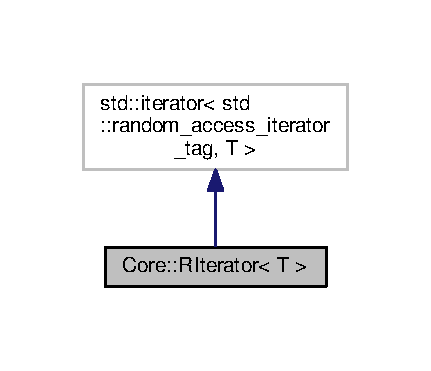
\includegraphics[width=207pt]{classCore_1_1RIterator__inherit__graph}
\end{center}
\end{figure}


Collaboration diagram for Core\+:\+:R\+Iterator$<$ T $>$\+:\nopagebreak
\begin{figure}[H]
\begin{center}
\leavevmode
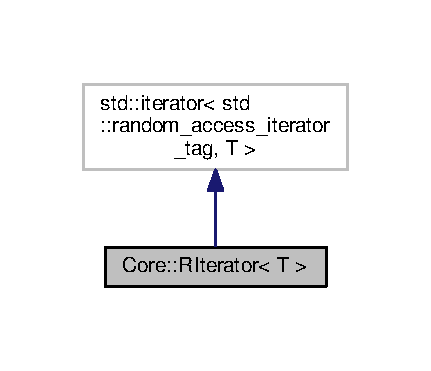
\includegraphics[width=207pt]{classCore_1_1RIterator__coll__graph}
\end{center}
\end{figure}
\subsection*{Public Member Functions}
\begin{DoxyCompactItemize}
\item 
\hyperlink{classCore_1_1RIterator_a78fd039a12776b6603ce00d3c735c376}{R\+Iterator} (T $\ast$ptr=nullptr)
\item 
\hyperlink{classCore_1_1RIterator_a705eaa2ee97becba55487af931c2569f}{R\+Iterator} (const \hyperlink{classCore_1_1RIterator}{R\+Iterator}$<$ T $>$ \&it)=default
\item 
\hyperlink{classCore_1_1RIterator_ab56f396bdd61ce2c898ca66f2a475673}{$\sim$\+R\+Iterator} ()
\item 
\hyperlink{classCore_1_1RIterator}{R\+Iterator}$<$ T $>$ \& \hyperlink{classCore_1_1RIterator_ad840f368edd2996e6980f94879c414f3}{operator=} (const \hyperlink{classCore_1_1RIterator}{R\+Iterator}$<$ T $>$ \&it)=default
\item 
\hyperlink{classCore_1_1RIterator}{R\+Iterator}$<$ T $>$ \& \hyperlink{classCore_1_1RIterator_a94e7649750026af99412ee0a080c783a}{operator=} (T $\ast$ptr)
\item 
\hyperlink{classCore_1_1RIterator_a2d7e2c6a0ee9d2559fbc919ef6f0f341}{operator bool} () const 
\item 
bool \hyperlink{classCore_1_1RIterator_acd463ba36d1020ec4516b1989b96b270}{operator==} (const \hyperlink{classCore_1_1RIterator}{R\+Iterator}$<$ T $>$ \&it) const 
\item 
bool \hyperlink{classCore_1_1RIterator_a49cb3082b5827297c06f5d3ce3cbd88a}{operator!=} (const \hyperlink{classCore_1_1RIterator}{R\+Iterator}$<$ T $>$ \&it) const 
\item 
\hyperlink{classCore_1_1RIterator}{R\+Iterator}$<$ T $>$ \& \hyperlink{classCore_1_1RIterator_a6362bde248a7123430f5cc180e181ae9}{operator+=} (const std\+::ptrdiff\+\_\+t \&movement)
\item 
\hyperlink{classCore_1_1RIterator}{R\+Iterator}$<$ T $>$ \& \hyperlink{classCore_1_1RIterator_a60ec58d55d871408f59707a1cd3211ed}{operator-\/=} (const std\+::ptrdiff\+\_\+t \&movement)
\item 
\hyperlink{classCore_1_1RIterator}{R\+Iterator}$<$ T $>$ \& \hyperlink{classCore_1_1RIterator_a42838da5641e16964b223285e7d2582c}{operator++} ()
\item 
\hyperlink{classCore_1_1RIterator}{R\+Iterator}$<$ T $>$ \& \hyperlink{classCore_1_1RIterator_a44ed38e2d3f689867c35efd944c53cec}{operator-\/-\/} ()
\item 
\hyperlink{classCore_1_1RIterator}{R\+Iterator}$<$ T $>$ \hyperlink{classCore_1_1RIterator_acc3b7d33ea79eb00fcddf94fea22019e}{operator++} (int)
\item 
\hyperlink{classCore_1_1RIterator}{R\+Iterator}$<$ T $>$ \hyperlink{classCore_1_1RIterator_a8dea5798b779678b79242cb52404319f}{operator-\/-\/} (int)
\item 
\hyperlink{classCore_1_1RIterator}{R\+Iterator}$<$ T $>$ \hyperlink{classCore_1_1RIterator_a7f63a17ca928bf7d7cdf212d657c69e0}{operator+} (const std\+::ptrdiff\+\_\+t \&movement)
\item 
\hyperlink{classCore_1_1RIterator}{R\+Iterator}$<$ T $>$ \hyperlink{classCore_1_1RIterator_aacf7e1c216fd628c5fe5a3367229c2be}{operator-\/} (const std\+::ptrdiff\+\_\+t \&movement)
\item 
std\+::ptrdiff\+\_\+t \hyperlink{classCore_1_1RIterator_a9eaec053392188bec54490eda23e58e7}{operator-\/} (const \hyperlink{classCore_1_1RIterator}{R\+Iterator}$<$ T $>$ \&it)
\item 
T \& \hyperlink{classCore_1_1RIterator_aaf429e98758b728b5eb7fcbfc8e44df8}{operator$\ast$} ()
\item 
const T \& \hyperlink{classCore_1_1RIterator_a7a8fb86cae284e57391ece18c13636e8}{operator$\ast$} () const 
\item 
T $\ast$ \hyperlink{classCore_1_1RIterator_ac3e3610863a3ad804e464fe9c5bbf34a}{operator-\/$>$} ()
\item 
T $\ast$ \hyperlink{classCore_1_1RIterator_aafbbd9cf4a6adbe6ab1eb256b417a410}{get\+Ptr} () const 
\item 
const T $\ast$ \hyperlink{classCore_1_1RIterator_a5afd5fabdaf34e57a2c5d076b289e5ae}{get\+Const\+Ptr} () const 
\end{DoxyCompactItemize}
\subsection*{Protected Attributes}
\begin{DoxyCompactItemize}
\item 
T $\ast$ \hyperlink{classCore_1_1RIterator_a573cae85de41fabc83d39edb28074091}{ptr\+\_\+}
\end{DoxyCompactItemize}


\subsection{Constructor \& Destructor Documentation}
\index{Core\+::\+R\+Iterator@{Core\+::\+R\+Iterator}!R\+Iterator@{R\+Iterator}}
\index{R\+Iterator@{R\+Iterator}!Core\+::\+R\+Iterator@{Core\+::\+R\+Iterator}}
\subsubsection[{\texorpdfstring{R\+Iterator(\+T $\ast$ptr=nullptr)}{RIterator(T *ptr=nullptr)}}]{\setlength{\rightskip}{0pt plus 5cm}template$<$typename T$>$ {\bf Core\+::\+R\+Iterator}$<$ T $>$\+::{\bf R\+Iterator} (
\begin{DoxyParamCaption}
\item[{T $\ast$}]{ptr = {\ttfamily nullptr}}
\end{DoxyParamCaption}
)\hspace{0.3cm}{\ttfamily [inline]}}\hypertarget{classCore_1_1RIterator_a78fd039a12776b6603ce00d3c735c376}{}\label{classCore_1_1RIterator_a78fd039a12776b6603ce00d3c735c376}
\index{Core\+::\+R\+Iterator@{Core\+::\+R\+Iterator}!R\+Iterator@{R\+Iterator}}
\index{R\+Iterator@{R\+Iterator}!Core\+::\+R\+Iterator@{Core\+::\+R\+Iterator}}
\subsubsection[{\texorpdfstring{R\+Iterator(const R\+Iterator$<$ T $>$ \&it)=default}{RIterator(const RIterator< T > &it)=default}}]{\setlength{\rightskip}{0pt plus 5cm}template$<$typename T$>$ {\bf Core\+::\+R\+Iterator}$<$ T $>$\+::{\bf R\+Iterator} (
\begin{DoxyParamCaption}
\item[{const {\bf R\+Iterator}$<$ T $>$ \&}]{it}
\end{DoxyParamCaption}
)\hspace{0.3cm}{\ttfamily [default]}}\hypertarget{classCore_1_1RIterator_a705eaa2ee97becba55487af931c2569f}{}\label{classCore_1_1RIterator_a705eaa2ee97becba55487af931c2569f}
\index{Core\+::\+R\+Iterator@{Core\+::\+R\+Iterator}!````~R\+Iterator@{$\sim$\+R\+Iterator}}
\index{````~R\+Iterator@{$\sim$\+R\+Iterator}!Core\+::\+R\+Iterator@{Core\+::\+R\+Iterator}}
\subsubsection[{\texorpdfstring{$\sim$\+R\+Iterator()}{~RIterator()}}]{\setlength{\rightskip}{0pt plus 5cm}template$<$typename T$>$ {\bf Core\+::\+R\+Iterator}$<$ T $>$\+::$\sim${\bf R\+Iterator} (
\begin{DoxyParamCaption}
{}
\end{DoxyParamCaption}
)\hspace{0.3cm}{\ttfamily [inline]}}\hypertarget{classCore_1_1RIterator_ab56f396bdd61ce2c898ca66f2a475673}{}\label{classCore_1_1RIterator_ab56f396bdd61ce2c898ca66f2a475673}


\subsection{Member Function Documentation}
\index{Core\+::\+R\+Iterator@{Core\+::\+R\+Iterator}!get\+Const\+Ptr@{get\+Const\+Ptr}}
\index{get\+Const\+Ptr@{get\+Const\+Ptr}!Core\+::\+R\+Iterator@{Core\+::\+R\+Iterator}}
\subsubsection[{\texorpdfstring{get\+Const\+Ptr() const }{getConstPtr() const }}]{\setlength{\rightskip}{0pt plus 5cm}template$<$typename T$>$ const T$\ast$ {\bf Core\+::\+R\+Iterator}$<$ T $>$\+::get\+Const\+Ptr (
\begin{DoxyParamCaption}
{}
\end{DoxyParamCaption}
) const\hspace{0.3cm}{\ttfamily [inline]}}\hypertarget{classCore_1_1RIterator_a5afd5fabdaf34e57a2c5d076b289e5ae}{}\label{classCore_1_1RIterator_a5afd5fabdaf34e57a2c5d076b289e5ae}
\index{Core\+::\+R\+Iterator@{Core\+::\+R\+Iterator}!get\+Ptr@{get\+Ptr}}
\index{get\+Ptr@{get\+Ptr}!Core\+::\+R\+Iterator@{Core\+::\+R\+Iterator}}
\subsubsection[{\texorpdfstring{get\+Ptr() const }{getPtr() const }}]{\setlength{\rightskip}{0pt plus 5cm}template$<$typename T$>$ T$\ast$ {\bf Core\+::\+R\+Iterator}$<$ T $>$\+::get\+Ptr (
\begin{DoxyParamCaption}
{}
\end{DoxyParamCaption}
) const\hspace{0.3cm}{\ttfamily [inline]}}\hypertarget{classCore_1_1RIterator_aafbbd9cf4a6adbe6ab1eb256b417a410}{}\label{classCore_1_1RIterator_aafbbd9cf4a6adbe6ab1eb256b417a410}
\index{Core\+::\+R\+Iterator@{Core\+::\+R\+Iterator}!operator bool@{operator bool}}
\index{operator bool@{operator bool}!Core\+::\+R\+Iterator@{Core\+::\+R\+Iterator}}
\subsubsection[{\texorpdfstring{operator bool() const }{operator bool() const }}]{\setlength{\rightskip}{0pt plus 5cm}template$<$typename T$>$ {\bf Core\+::\+R\+Iterator}$<$ T $>$\+::operator bool (
\begin{DoxyParamCaption}
{}
\end{DoxyParamCaption}
) const\hspace{0.3cm}{\ttfamily [inline]}}\hypertarget{classCore_1_1RIterator_a2d7e2c6a0ee9d2559fbc919ef6f0f341}{}\label{classCore_1_1RIterator_a2d7e2c6a0ee9d2559fbc919ef6f0f341}
\index{Core\+::\+R\+Iterator@{Core\+::\+R\+Iterator}!operator"!=@{operator"!=}}
\index{operator"!=@{operator"!=}!Core\+::\+R\+Iterator@{Core\+::\+R\+Iterator}}
\subsubsection[{\texorpdfstring{operator"!=(const R\+Iterator$<$ T $>$ \&it) const }{operator!=(const RIterator< T > &it) const }}]{\setlength{\rightskip}{0pt plus 5cm}template$<$typename T$>$ bool {\bf Core\+::\+R\+Iterator}$<$ T $>$\+::operator!= (
\begin{DoxyParamCaption}
\item[{const {\bf R\+Iterator}$<$ T $>$ \&}]{it}
\end{DoxyParamCaption}
) const\hspace{0.3cm}{\ttfamily [inline]}}\hypertarget{classCore_1_1RIterator_a49cb3082b5827297c06f5d3ce3cbd88a}{}\label{classCore_1_1RIterator_a49cb3082b5827297c06f5d3ce3cbd88a}
\index{Core\+::\+R\+Iterator@{Core\+::\+R\+Iterator}!operator$\ast$@{operator$\ast$}}
\index{operator$\ast$@{operator$\ast$}!Core\+::\+R\+Iterator@{Core\+::\+R\+Iterator}}
\subsubsection[{\texorpdfstring{operator$\ast$()}{operator*()}}]{\setlength{\rightskip}{0pt plus 5cm}template$<$typename T$>$ T\& {\bf Core\+::\+R\+Iterator}$<$ T $>$\+::operator$\ast$ (
\begin{DoxyParamCaption}
{}
\end{DoxyParamCaption}
)\hspace{0.3cm}{\ttfamily [inline]}}\hypertarget{classCore_1_1RIterator_aaf429e98758b728b5eb7fcbfc8e44df8}{}\label{classCore_1_1RIterator_aaf429e98758b728b5eb7fcbfc8e44df8}
\index{Core\+::\+R\+Iterator@{Core\+::\+R\+Iterator}!operator$\ast$@{operator$\ast$}}
\index{operator$\ast$@{operator$\ast$}!Core\+::\+R\+Iterator@{Core\+::\+R\+Iterator}}
\subsubsection[{\texorpdfstring{operator$\ast$() const }{operator*() const }}]{\setlength{\rightskip}{0pt plus 5cm}template$<$typename T$>$ const T\& {\bf Core\+::\+R\+Iterator}$<$ T $>$\+::operator$\ast$ (
\begin{DoxyParamCaption}
{}
\end{DoxyParamCaption}
) const\hspace{0.3cm}{\ttfamily [inline]}}\hypertarget{classCore_1_1RIterator_a7a8fb86cae284e57391ece18c13636e8}{}\label{classCore_1_1RIterator_a7a8fb86cae284e57391ece18c13636e8}
\index{Core\+::\+R\+Iterator@{Core\+::\+R\+Iterator}!operator+@{operator+}}
\index{operator+@{operator+}!Core\+::\+R\+Iterator@{Core\+::\+R\+Iterator}}
\subsubsection[{\texorpdfstring{operator+(const std\+::ptrdiff\+\_\+t \&movement)}{operator+(const std::ptrdiff_t &movement)}}]{\setlength{\rightskip}{0pt plus 5cm}template$<$typename T$>$ {\bf R\+Iterator}$<$T$>$ {\bf Core\+::\+R\+Iterator}$<$ T $>$\+::operator+ (
\begin{DoxyParamCaption}
\item[{const std\+::ptrdiff\+\_\+t \&}]{movement}
\end{DoxyParamCaption}
)\hspace{0.3cm}{\ttfamily [inline]}}\hypertarget{classCore_1_1RIterator_a7f63a17ca928bf7d7cdf212d657c69e0}{}\label{classCore_1_1RIterator_a7f63a17ca928bf7d7cdf212d657c69e0}
\index{Core\+::\+R\+Iterator@{Core\+::\+R\+Iterator}!operator++@{operator++}}
\index{operator++@{operator++}!Core\+::\+R\+Iterator@{Core\+::\+R\+Iterator}}
\subsubsection[{\texorpdfstring{operator++()}{operator++()}}]{\setlength{\rightskip}{0pt plus 5cm}template$<$typename T$>$ {\bf R\+Iterator}$<$T$>$\& {\bf Core\+::\+R\+Iterator}$<$ T $>$\+::operator++ (
\begin{DoxyParamCaption}
{}
\end{DoxyParamCaption}
)\hspace{0.3cm}{\ttfamily [inline]}}\hypertarget{classCore_1_1RIterator_a42838da5641e16964b223285e7d2582c}{}\label{classCore_1_1RIterator_a42838da5641e16964b223285e7d2582c}
\index{Core\+::\+R\+Iterator@{Core\+::\+R\+Iterator}!operator++@{operator++}}
\index{operator++@{operator++}!Core\+::\+R\+Iterator@{Core\+::\+R\+Iterator}}
\subsubsection[{\texorpdfstring{operator++(int)}{operator++(int)}}]{\setlength{\rightskip}{0pt plus 5cm}template$<$typename T$>$ {\bf R\+Iterator}$<$T$>$ {\bf Core\+::\+R\+Iterator}$<$ T $>$\+::operator++ (
\begin{DoxyParamCaption}
\item[{int}]{}
\end{DoxyParamCaption}
)\hspace{0.3cm}{\ttfamily [inline]}}\hypertarget{classCore_1_1RIterator_acc3b7d33ea79eb00fcddf94fea22019e}{}\label{classCore_1_1RIterator_acc3b7d33ea79eb00fcddf94fea22019e}
\index{Core\+::\+R\+Iterator@{Core\+::\+R\+Iterator}!operator+=@{operator+=}}
\index{operator+=@{operator+=}!Core\+::\+R\+Iterator@{Core\+::\+R\+Iterator}}
\subsubsection[{\texorpdfstring{operator+=(const std\+::ptrdiff\+\_\+t \&movement)}{operator+=(const std::ptrdiff_t &movement)}}]{\setlength{\rightskip}{0pt plus 5cm}template$<$typename T$>$ {\bf R\+Iterator}$<$T$>$\& {\bf Core\+::\+R\+Iterator}$<$ T $>$\+::operator+= (
\begin{DoxyParamCaption}
\item[{const std\+::ptrdiff\+\_\+t \&}]{movement}
\end{DoxyParamCaption}
)\hspace{0.3cm}{\ttfamily [inline]}}\hypertarget{classCore_1_1RIterator_a6362bde248a7123430f5cc180e181ae9}{}\label{classCore_1_1RIterator_a6362bde248a7123430f5cc180e181ae9}
\index{Core\+::\+R\+Iterator@{Core\+::\+R\+Iterator}!operator-\/@{operator-\/}}
\index{operator-\/@{operator-\/}!Core\+::\+R\+Iterator@{Core\+::\+R\+Iterator}}
\subsubsection[{\texorpdfstring{operator-\/(const std\+::ptrdiff\+\_\+t \&movement)}{operator-(const std::ptrdiff_t &movement)}}]{\setlength{\rightskip}{0pt plus 5cm}template$<$typename T$>$ {\bf R\+Iterator}$<$T$>$ {\bf Core\+::\+R\+Iterator}$<$ T $>$\+::operator-\/ (
\begin{DoxyParamCaption}
\item[{const std\+::ptrdiff\+\_\+t \&}]{movement}
\end{DoxyParamCaption}
)\hspace{0.3cm}{\ttfamily [inline]}}\hypertarget{classCore_1_1RIterator_aacf7e1c216fd628c5fe5a3367229c2be}{}\label{classCore_1_1RIterator_aacf7e1c216fd628c5fe5a3367229c2be}
\index{Core\+::\+R\+Iterator@{Core\+::\+R\+Iterator}!operator-\/@{operator-\/}}
\index{operator-\/@{operator-\/}!Core\+::\+R\+Iterator@{Core\+::\+R\+Iterator}}
\subsubsection[{\texorpdfstring{operator-\/(const R\+Iterator$<$ T $>$ \&it)}{operator-(const RIterator< T > &it)}}]{\setlength{\rightskip}{0pt plus 5cm}template$<$typename T$>$ std\+::ptrdiff\+\_\+t {\bf Core\+::\+R\+Iterator}$<$ T $>$\+::operator-\/ (
\begin{DoxyParamCaption}
\item[{const {\bf R\+Iterator}$<$ T $>$ \&}]{it}
\end{DoxyParamCaption}
)\hspace{0.3cm}{\ttfamily [inline]}}\hypertarget{classCore_1_1RIterator_a9eaec053392188bec54490eda23e58e7}{}\label{classCore_1_1RIterator_a9eaec053392188bec54490eda23e58e7}
\index{Core\+::\+R\+Iterator@{Core\+::\+R\+Iterator}!operator-\/-\/@{operator-\/-\/}}
\index{operator-\/-\/@{operator-\/-\/}!Core\+::\+R\+Iterator@{Core\+::\+R\+Iterator}}
\subsubsection[{\texorpdfstring{operator-\/-\/()}{operator--()}}]{\setlength{\rightskip}{0pt plus 5cm}template$<$typename T$>$ {\bf R\+Iterator}$<$T$>$\& {\bf Core\+::\+R\+Iterator}$<$ T $>$\+::operator-\/-\/ (
\begin{DoxyParamCaption}
{}
\end{DoxyParamCaption}
)\hspace{0.3cm}{\ttfamily [inline]}}\hypertarget{classCore_1_1RIterator_a44ed38e2d3f689867c35efd944c53cec}{}\label{classCore_1_1RIterator_a44ed38e2d3f689867c35efd944c53cec}
\index{Core\+::\+R\+Iterator@{Core\+::\+R\+Iterator}!operator-\/-\/@{operator-\/-\/}}
\index{operator-\/-\/@{operator-\/-\/}!Core\+::\+R\+Iterator@{Core\+::\+R\+Iterator}}
\subsubsection[{\texorpdfstring{operator-\/-\/(int)}{operator--(int)}}]{\setlength{\rightskip}{0pt plus 5cm}template$<$typename T$>$ {\bf R\+Iterator}$<$T$>$ {\bf Core\+::\+R\+Iterator}$<$ T $>$\+::operator-\/-\/ (
\begin{DoxyParamCaption}
\item[{int}]{}
\end{DoxyParamCaption}
)\hspace{0.3cm}{\ttfamily [inline]}}\hypertarget{classCore_1_1RIterator_a8dea5798b779678b79242cb52404319f}{}\label{classCore_1_1RIterator_a8dea5798b779678b79242cb52404319f}
\index{Core\+::\+R\+Iterator@{Core\+::\+R\+Iterator}!operator-\/=@{operator-\/=}}
\index{operator-\/=@{operator-\/=}!Core\+::\+R\+Iterator@{Core\+::\+R\+Iterator}}
\subsubsection[{\texorpdfstring{operator-\/=(const std\+::ptrdiff\+\_\+t \&movement)}{operator-=(const std::ptrdiff_t &movement)}}]{\setlength{\rightskip}{0pt plus 5cm}template$<$typename T$>$ {\bf R\+Iterator}$<$T$>$\& {\bf Core\+::\+R\+Iterator}$<$ T $>$\+::operator-\/= (
\begin{DoxyParamCaption}
\item[{const std\+::ptrdiff\+\_\+t \&}]{movement}
\end{DoxyParamCaption}
)\hspace{0.3cm}{\ttfamily [inline]}}\hypertarget{classCore_1_1RIterator_a60ec58d55d871408f59707a1cd3211ed}{}\label{classCore_1_1RIterator_a60ec58d55d871408f59707a1cd3211ed}
\index{Core\+::\+R\+Iterator@{Core\+::\+R\+Iterator}!operator-\/$>$@{operator-\/$>$}}
\index{operator-\/$>$@{operator-\/$>$}!Core\+::\+R\+Iterator@{Core\+::\+R\+Iterator}}
\subsubsection[{\texorpdfstring{operator-\/$>$()}{operator->()}}]{\setlength{\rightskip}{0pt plus 5cm}template$<$typename T$>$ T$\ast$ {\bf Core\+::\+R\+Iterator}$<$ T $>$\+::operator-\/$>$ (
\begin{DoxyParamCaption}
{}
\end{DoxyParamCaption}
)\hspace{0.3cm}{\ttfamily [inline]}}\hypertarget{classCore_1_1RIterator_ac3e3610863a3ad804e464fe9c5bbf34a}{}\label{classCore_1_1RIterator_ac3e3610863a3ad804e464fe9c5bbf34a}
\index{Core\+::\+R\+Iterator@{Core\+::\+R\+Iterator}!operator=@{operator=}}
\index{operator=@{operator=}!Core\+::\+R\+Iterator@{Core\+::\+R\+Iterator}}
\subsubsection[{\texorpdfstring{operator=(const R\+Iterator$<$ T $>$ \&it)=default}{operator=(const RIterator< T > &it)=default}}]{\setlength{\rightskip}{0pt plus 5cm}template$<$typename T$>$ {\bf R\+Iterator}$<$T$>$\& {\bf Core\+::\+R\+Iterator}$<$ T $>$\+::operator= (
\begin{DoxyParamCaption}
\item[{const {\bf R\+Iterator}$<$ T $>$ \&}]{it}
\end{DoxyParamCaption}
)\hspace{0.3cm}{\ttfamily [default]}}\hypertarget{classCore_1_1RIterator_ad840f368edd2996e6980f94879c414f3}{}\label{classCore_1_1RIterator_ad840f368edd2996e6980f94879c414f3}
\index{Core\+::\+R\+Iterator@{Core\+::\+R\+Iterator}!operator=@{operator=}}
\index{operator=@{operator=}!Core\+::\+R\+Iterator@{Core\+::\+R\+Iterator}}
\subsubsection[{\texorpdfstring{operator=(\+T $\ast$ptr)}{operator=(T *ptr)}}]{\setlength{\rightskip}{0pt plus 5cm}template$<$typename T$>$ {\bf R\+Iterator}$<$T$>$\& {\bf Core\+::\+R\+Iterator}$<$ T $>$\+::operator= (
\begin{DoxyParamCaption}
\item[{T $\ast$}]{ptr}
\end{DoxyParamCaption}
)\hspace{0.3cm}{\ttfamily [inline]}}\hypertarget{classCore_1_1RIterator_a94e7649750026af99412ee0a080c783a}{}\label{classCore_1_1RIterator_a94e7649750026af99412ee0a080c783a}
\index{Core\+::\+R\+Iterator@{Core\+::\+R\+Iterator}!operator==@{operator==}}
\index{operator==@{operator==}!Core\+::\+R\+Iterator@{Core\+::\+R\+Iterator}}
\subsubsection[{\texorpdfstring{operator==(const R\+Iterator$<$ T $>$ \&it) const }{operator==(const RIterator< T > &it) const }}]{\setlength{\rightskip}{0pt plus 5cm}template$<$typename T$>$ bool {\bf Core\+::\+R\+Iterator}$<$ T $>$\+::operator== (
\begin{DoxyParamCaption}
\item[{const {\bf R\+Iterator}$<$ T $>$ \&}]{it}
\end{DoxyParamCaption}
) const\hspace{0.3cm}{\ttfamily [inline]}}\hypertarget{classCore_1_1RIterator_acd463ba36d1020ec4516b1989b96b270}{}\label{classCore_1_1RIterator_acd463ba36d1020ec4516b1989b96b270}


\subsection{Member Data Documentation}
\index{Core\+::\+R\+Iterator@{Core\+::\+R\+Iterator}!ptr\+\_\+@{ptr\+\_\+}}
\index{ptr\+\_\+@{ptr\+\_\+}!Core\+::\+R\+Iterator@{Core\+::\+R\+Iterator}}
\subsubsection[{\texorpdfstring{ptr\+\_\+}{ptr_}}]{\setlength{\rightskip}{0pt plus 5cm}template$<$typename T$>$ T$\ast$ {\bf Core\+::\+R\+Iterator}$<$ T $>$\+::ptr\+\_\+\hspace{0.3cm}{\ttfamily [protected]}}\hypertarget{classCore_1_1RIterator_a573cae85de41fabc83d39edb28074091}{}\label{classCore_1_1RIterator_a573cae85de41fabc83d39edb28074091}


The documentation for this class was generated from the following file\+:\begin{DoxyCompactItemize}
\item 
\hyperlink{riterator_8h}{riterator.\+h}\end{DoxyCompactItemize}

\chapter{File Documentation}
\hypertarget{cmysql__database_8cpp}{}\section{cmysql\+\_\+database.\+cpp File Reference}
\label{cmysql__database_8cpp}\index{cmysql\+\_\+database.\+cpp@{cmysql\+\_\+database.\+cpp}}
{\ttfamily \#include $<$string$>$}\\*
{\ttfamily \#include \char`\"{}cmysql\+\_\+database.\+h\char`\"{}}\\*
{\ttfamily \#include $<$exception$>$}\\*
{\ttfamily \#include $<$stdexcept$>$}\\*
Include dependency graph for cmysql\+\_\+database.\+cpp\+:\nopagebreak
\begin{figure}[H]
\begin{center}
\leavevmode
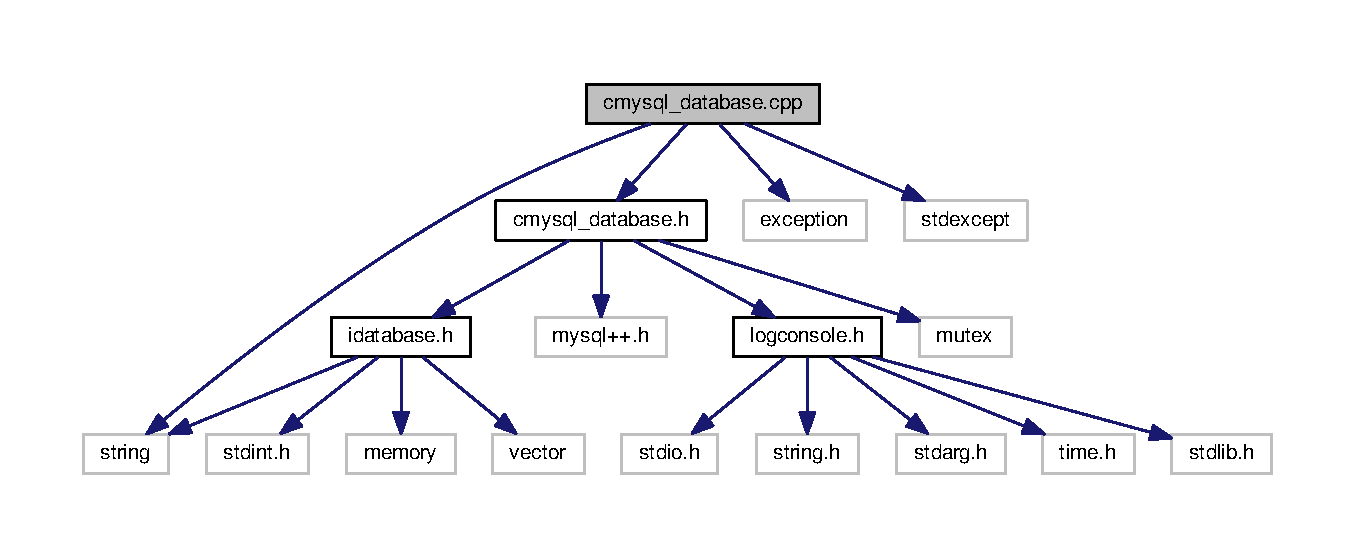
\includegraphics[width=350pt]{cmysql__database_8cpp__incl}
\end{center}
\end{figure}
\subsection*{Namespaces}
\begin{DoxyCompactItemize}
\item 
 \hyperlink{namespaceCore}{Core}
\end{DoxyCompactItemize}

\hypertarget{cmysql__database_8h}{}\section{cmysql\+\_\+database.\+h File Reference}
\label{cmysql__database_8h}\index{cmysql\+\_\+database.\+h@{cmysql\+\_\+database.\+h}}
{\ttfamily \#include \char`\"{}idatabase.\+h\char`\"{}}\\*
{\ttfamily \#include $<$mysql++.\+h$>$}\\*
{\ttfamily \#include \char`\"{}logconsole.\+h\char`\"{}}\\*
{\ttfamily \#include $<$mutex$>$}\\*
Include dependency graph for cmysql\+\_\+database.\+h\+:\nopagebreak
\begin{figure}[H]
\begin{center}
\leavevmode
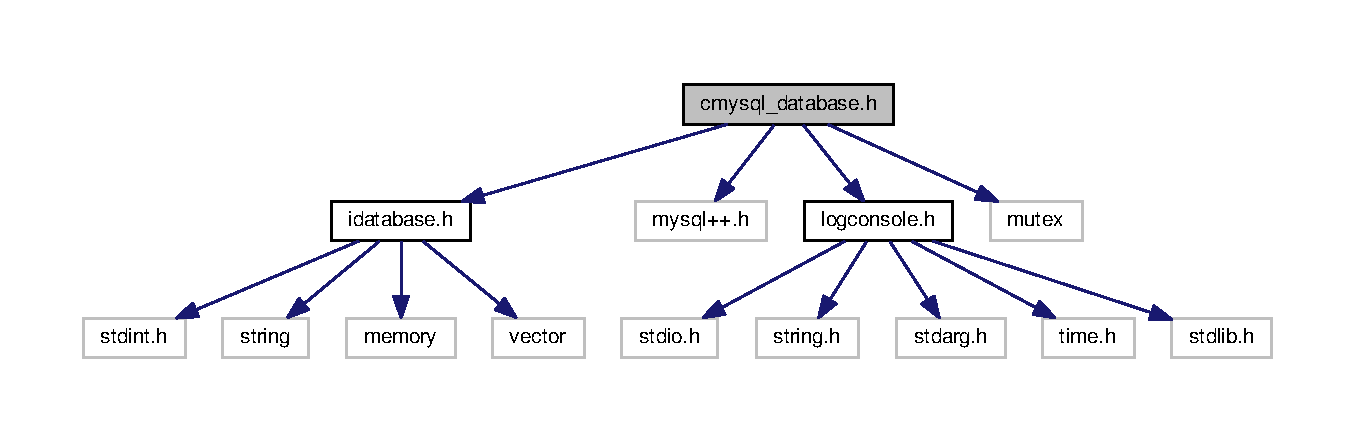
\includegraphics[width=350pt]{cmysql__database_8h__incl}
\end{center}
\end{figure}
This graph shows which files directly or indirectly include this file\+:\nopagebreak
\begin{figure}[H]
\begin{center}
\leavevmode
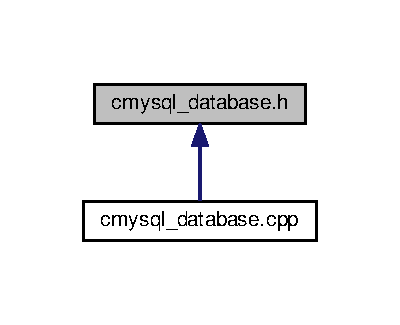
\includegraphics[width=192pt]{cmysql__database_8h__dep__incl}
\end{center}
\end{figure}
\subsection*{Classes}
\begin{DoxyCompactItemize}
\item 
class \hyperlink{classCore_1_1CMySQL__Row}{Core\+::\+C\+My\+S\+Q\+L\+\_\+\+Row}
\item 
class \hyperlink{classCore_1_1CMySQL__Result}{Core\+::\+C\+My\+S\+Q\+L\+\_\+\+Result}
\item 
class \hyperlink{classCore_1_1CMySQL__Database}{Core\+::\+C\+My\+S\+Q\+L\+\_\+\+Database}
\end{DoxyCompactItemize}
\subsection*{Namespaces}
\begin{DoxyCompactItemize}
\item 
 \hyperlink{namespaceCore}{Core}
\end{DoxyCompactItemize}

\hypertarget{cnetwork__asio_8cpp}{}\section{cnetwork\+\_\+asio.\+cpp File Reference}
\label{cnetwork__asio_8cpp}\index{cnetwork\+\_\+asio.\+cpp@{cnetwork\+\_\+asio.\+cpp}}
{\ttfamily \#include $<$cstdlib$>$}\\*
{\ttfamily \#include $<$iostream$>$}\\*
{\ttfamily \#include $<$thread$>$}\\*
{\ttfamily \#include \char`\"{}logconsole.\+h\char`\"{}}\\*
{\ttfamily \#include \char`\"{}cnetwork\+\_\+asio.\+h\char`\"{}}\\*
Include dependency graph for cnetwork\+\_\+asio.\+cpp\+:\nopagebreak
\begin{figure}[H]
\begin{center}
\leavevmode
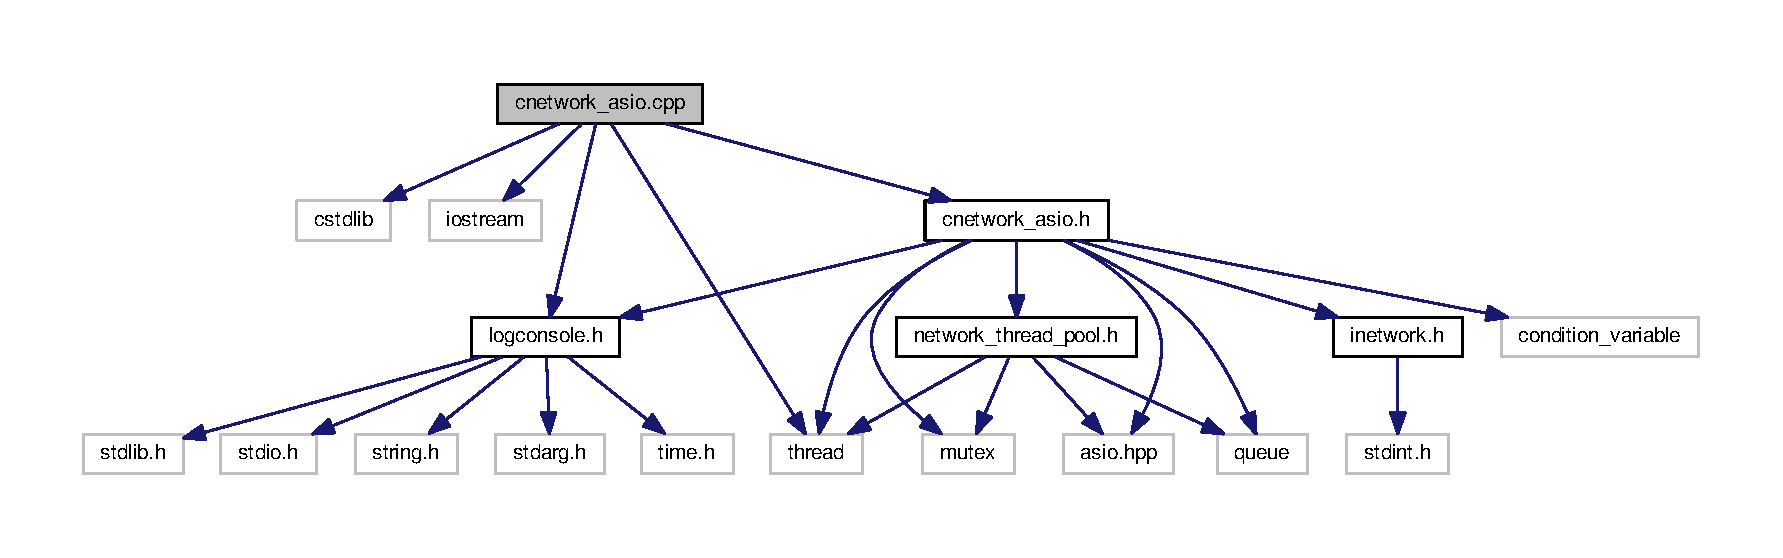
\includegraphics[width=350pt]{cnetwork__asio_8cpp__incl}
\end{center}
\end{figure}
\subsection*{Namespaces}
\begin{DoxyCompactItemize}
\item 
 \hyperlink{namespaceCore}{Core}
\end{DoxyCompactItemize}

\hypertarget{cnetwork__asio_8h}{}\section{cnetwork\+\_\+asio.\+h File Reference}
\label{cnetwork__asio_8h}\index{cnetwork\+\_\+asio.\+h@{cnetwork\+\_\+asio.\+h}}
{\ttfamily \#include $<$asio.\+hpp$>$}\\*
{\ttfamily \#include $<$queue$>$}\\*
{\ttfamily \#include $<$mutex$>$}\\*
{\ttfamily \#include $<$thread$>$}\\*
{\ttfamily \#include $<$condition\+\_\+variable$>$}\\*
{\ttfamily \#include \char`\"{}inetwork.\+h\char`\"{}}\\*
{\ttfamily \#include \char`\"{}logconsole.\+h\char`\"{}}\\*
{\ttfamily \#include \char`\"{}network\+\_\+thread\+\_\+pool.\+h\char`\"{}}\\*
Include dependency graph for cnetwork\+\_\+asio.\+h\+:\nopagebreak
\begin{figure}[H]
\begin{center}
\leavevmode
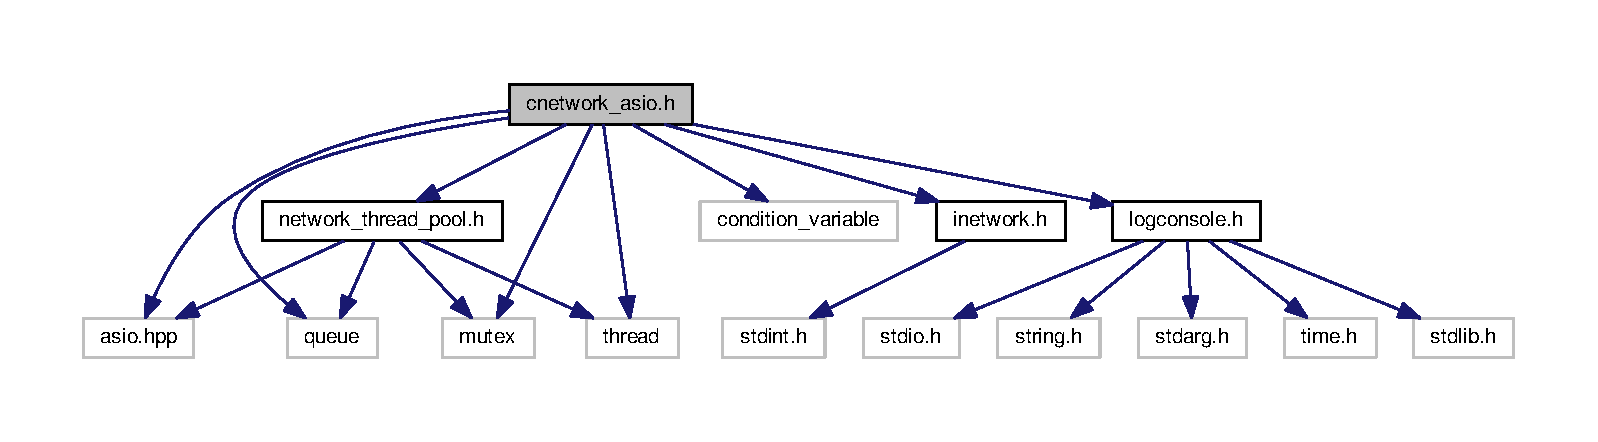
\includegraphics[width=350pt]{cnetwork__asio_8h__incl}
\end{center}
\end{figure}
This graph shows which files directly or indirectly include this file\+:\nopagebreak
\begin{figure}[H]
\begin{center}
\leavevmode
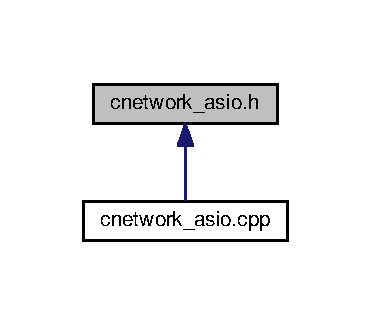
\includegraphics[width=178pt]{cnetwork__asio_8h__dep__incl}
\end{center}
\end{figure}
\subsection*{Classes}
\begin{DoxyCompactItemize}
\item 
class \hyperlink{classCore_1_1CNetwork__Asio}{Core\+::\+C\+Network\+\_\+\+Asio}
\end{DoxyCompactItemize}
\subsection*{Namespaces}
\begin{DoxyCompactItemize}
\item 
 \hyperlink{namespaceCore}{Core}
\end{DoxyCompactItemize}
\subsection*{Macros}
\begin{DoxyCompactItemize}
\item 
\#define \hyperlink{cnetwork__asio_8h_a879456c3b8e2853f7044d764e9c180d4}{M\+A\+X\+\_\+\+P\+A\+C\+K\+E\+T\+\_\+\+S\+I\+ZE}~0x7\+FF
\end{DoxyCompactItemize}


\subsection{Macro Definition Documentation}
\index{cnetwork\+\_\+asio.\+h@{cnetwork\+\_\+asio.\+h}!M\+A\+X\+\_\+\+P\+A\+C\+K\+E\+T\+\_\+\+S\+I\+ZE@{M\+A\+X\+\_\+\+P\+A\+C\+K\+E\+T\+\_\+\+S\+I\+ZE}}
\index{M\+A\+X\+\_\+\+P\+A\+C\+K\+E\+T\+\_\+\+S\+I\+ZE@{M\+A\+X\+\_\+\+P\+A\+C\+K\+E\+T\+\_\+\+S\+I\+ZE}!cnetwork\+\_\+asio.\+h@{cnetwork\+\_\+asio.\+h}}
\subsubsection[{\texorpdfstring{M\+A\+X\+\_\+\+P\+A\+C\+K\+E\+T\+\_\+\+S\+I\+ZE}{MAX_PACKET_SIZE}}]{\setlength{\rightskip}{0pt plus 5cm}\#define M\+A\+X\+\_\+\+P\+A\+C\+K\+E\+T\+\_\+\+S\+I\+ZE~0x7\+FF}\hypertarget{cnetwork__asio_8h_a879456c3b8e2853f7044d764e9c180d4}{}\label{cnetwork__asio_8h_a879456c3b8e2853f7044d764e9c180d4}

\hypertarget{config_8cpp}{}\section{config.\+cpp File Reference}
\label{config_8cpp}\index{config.\+cpp@{config.\+cpp}}
{\ttfamily \#include \char`\"{}config.\+h\char`\"{}}\\*
{\ttfamily \#include $<$fstream$>$}\\*
{\ttfamily \#include $<$iostream$>$}\\*
{\ttfamily \#include $<$exception$>$}\\*
Include dependency graph for config.\+cpp\+:\nopagebreak
\begin{figure}[H]
\begin{center}
\leavevmode
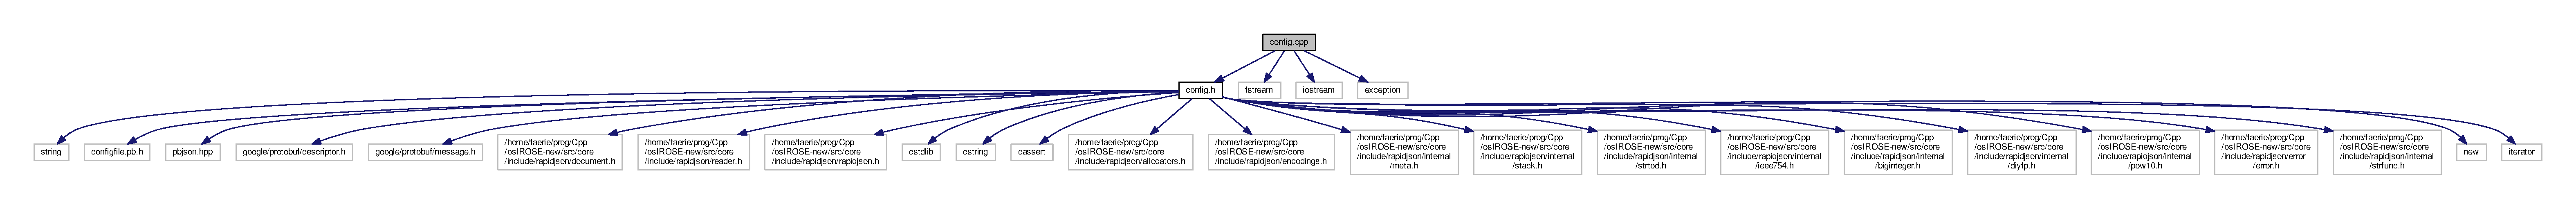
\includegraphics[width=350pt]{config_8cpp__incl}
\end{center}
\end{figure}

\hypertarget{config_8h}{}\section{config.\+h File Reference}
\label{config_8h}\index{config.\+h@{config.\+h}}
{\ttfamily \#include $<$string$>$}\\*
{\ttfamily \#include \char`\"{}configfile.\+pb.\+h\char`\"{}}\\*
{\ttfamily \#include \char`\"{}pbjson.\+hpp\char`\"{}}\\*
Include dependency graph for config.\+h\+:\nopagebreak
\begin{figure}[H]
\begin{center}
\leavevmode
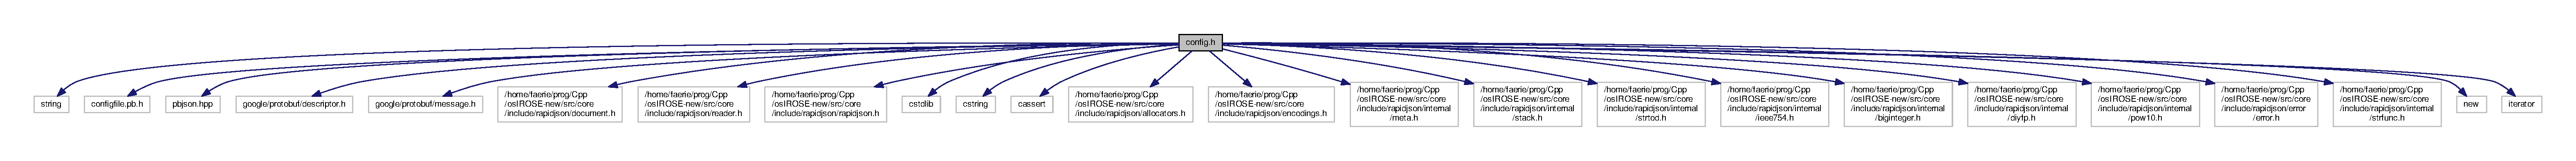
\includegraphics[width=350pt]{config_8h__incl}
\end{center}
\end{figure}
This graph shows which files directly or indirectly include this file\+:\nopagebreak
\begin{figure}[H]
\begin{center}
\leavevmode
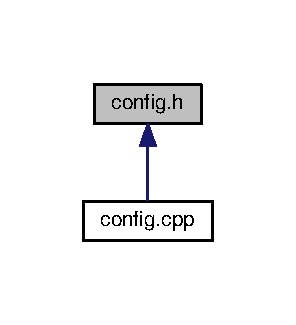
\includegraphics[width=142pt]{config_8h__dep__incl}
\end{center}
\end{figure}
\subsection*{Classes}
\begin{DoxyCompactItemize}
\item 
class \hyperlink{classConfig}{Config}
\end{DoxyCompactItemize}

\hypertarget{idatabase_8h}{}\section{idatabase.\+h File Reference}
\label{idatabase_8h}\index{idatabase.\+h@{idatabase.\+h}}
{\ttfamily \#include $<$stdint.\+h$>$}\\*
{\ttfamily \#include $<$string$>$}\\*
{\ttfamily \#include $<$memory$>$}\\*
{\ttfamily \#include $<$vector$>$}\\*
Include dependency graph for idatabase.\+h\+:\nopagebreak
\begin{figure}[H]
\begin{center}
\leavevmode
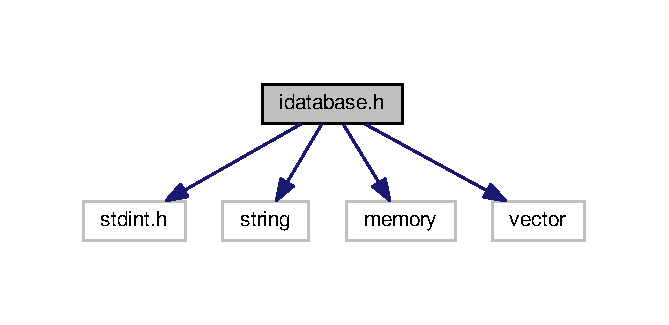
\includegraphics[width=321pt]{idatabase_8h__incl}
\end{center}
\end{figure}
This graph shows which files directly or indirectly include this file\+:\nopagebreak
\begin{figure}[H]
\begin{center}
\leavevmode
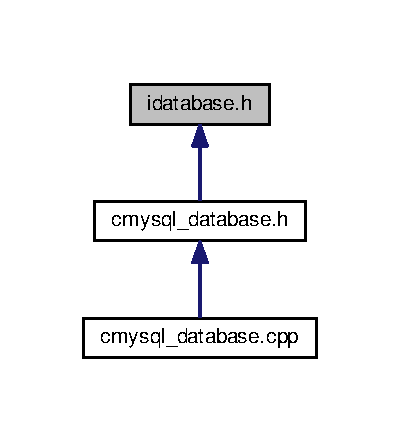
\includegraphics[width=192pt]{idatabase_8h__dep__incl}
\end{center}
\end{figure}
\subsection*{Classes}
\begin{DoxyCompactItemize}
\item 
class \hyperlink{classCore_1_1IRow}{Core\+::\+I\+Row}
\item 
class \hyperlink{classCore_1_1IResult}{Core\+::\+I\+Result}
\item 
class \hyperlink{classCore_1_1IDatabase}{Core\+::\+I\+Database}
\end{DoxyCompactItemize}
\subsection*{Namespaces}
\begin{DoxyCompactItemize}
\item 
 \hyperlink{namespaceCore}{Core}
\end{DoxyCompactItemize}

\hypertarget{inetwork_8h}{}\section{inetwork.\+h File Reference}
\label{inetwork_8h}\index{inetwork.\+h@{inetwork.\+h}}
{\ttfamily \#include $<$stdint.\+h$>$}\\*
Include dependency graph for inetwork.\+h\+:\nopagebreak
\begin{figure}[H]
\begin{center}
\leavevmode
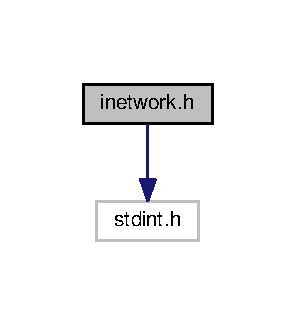
\includegraphics[width=142pt]{inetwork_8h__incl}
\end{center}
\end{figure}
This graph shows which files directly or indirectly include this file\+:\nopagebreak
\begin{figure}[H]
\begin{center}
\leavevmode
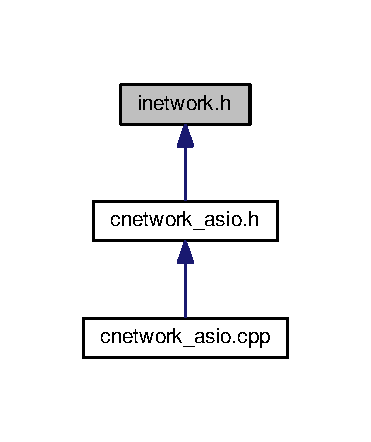
\includegraphics[width=178pt]{inetwork_8h__dep__incl}
\end{center}
\end{figure}
\subsection*{Classes}
\begin{DoxyCompactItemize}
\item 
class \hyperlink{classINetwork}{I\+Network}
\end{DoxyCompactItemize}

\hypertarget{logconsole_8cpp}{}\section{logconsole.\+cpp File Reference}
\label{logconsole_8cpp}\index{logconsole.\+cpp@{logconsole.\+cpp}}
{\ttfamily \#include $<$mutex$>$}\\*
{\ttfamily \#include \char`\"{}logconsole.\+h\char`\"{}}\\*
Include dependency graph for logconsole.\+cpp\+:\nopagebreak
\begin{figure}[H]
\begin{center}
\leavevmode
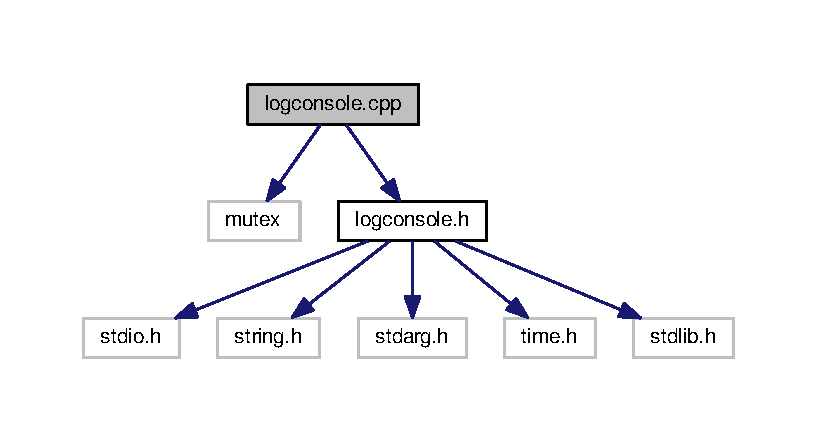
\includegraphics[width=350pt]{logconsole_8cpp__incl}
\end{center}
\end{figure}
\subsection*{Namespaces}
\begin{DoxyCompactItemize}
\item 
 \hyperlink{namespaceCore}{Core}
\end{DoxyCompactItemize}
\subsection*{Macros}
\begin{DoxyCompactItemize}
\item 
\#define \hyperlink{logconsole_8cpp_a2facdfca371afebb3364c87fae328d95}{S\+B\+U\+F\+\_\+\+S\+I\+ZE}~2048
\item 
\#define \hyperlink{logconsole_8cpp_a2d25bcd37166cc98f0d823cdb8c553ef}{uint8}~unsigned char
\item 
\#define \hyperlink{logconsole_8cpp_a9695cf1104606879c5d3f0221635a069}{uint32}~unsigned long
\item 
\#define \hyperlink{logconsole_8cpp_af62e66227ee4bc21dc19daf0f55f45a7}{N\+E\+W\+B\+UF}(buf)
\item 
\#define \hyperlink{logconsole_8cpp_a6c3d088b0a89908a6244864824623799}{B\+U\+F\+V\+P\+R\+I\+N\+TF}(buf,  fmt,  args)
\item 
\#define \hyperlink{logconsole_8cpp_a41152762b11d02d1db3448a92f91b71f}{B\+U\+F\+V\+AL}(buf)~buf.\+v\+\_\+
\item 
\#define \hyperlink{logconsole_8cpp_aa1718d5aeea7b902569252f6c6802bc6}{B\+U\+F\+L\+EN}(buf)~buf.\+l\+\_\+
\item 
\#define \hyperlink{logconsole_8cpp_a6d59088b73a3126218b9bef83f4abc8a}{F\+R\+E\+E\+B\+UF}(buf)
\item 
\#define \hyperlink{logconsole_8cpp_a6582f05711954011e2ceacc62d6ebad2}{I\+S\+D\+I\+G\+IT}(d)~(d $>$= \textquotesingle{}0\textquotesingle{} \&\& d $<$= \textquotesingle{}9\textquotesingle{})
\item 
\#define \hyperlink{logconsole_8cpp_afeee3cbb310f621900e0b8e455155b92}{is\+\_\+console}(file)~(0 != isatty(fileno(file)))
\item 
\#define \hyperlink{logconsole_8cpp_aaf117506502202ece7cb35a86682e66f}{F\+F\+L\+U\+SH}~fflush
\item 
\#define \hyperlink{logconsole_8cpp_a8875037d0772a4fc34516f1e03d7e238}{S\+T\+D\+O\+UT}~stdout
\item 
\#define \hyperlink{logconsole_8cpp_a3a540e3eef339eec06aff31c4ba1eb25}{S\+T\+D\+E\+RR}~stderr
\end{DoxyCompactItemize}
\subsection*{Functions}
\begin{DoxyCompactItemize}
\item 
int \hyperlink{namespaceCore_ac841f812f5ff61ba38222f7d441509d3}{Core\+::clprintf} (const char $\ast$fmt,...)
\item 
int \hyperlink{namespaceCore_a630dcb213704b7856eec935d8695ffe9}{Core\+::clvprintf} (const char $\ast$fmt, va\+\_\+list)
\end{DoxyCompactItemize}


\subsection{Macro Definition Documentation}
\index{logconsole.\+cpp@{logconsole.\+cpp}!B\+U\+F\+L\+EN@{B\+U\+F\+L\+EN}}
\index{B\+U\+F\+L\+EN@{B\+U\+F\+L\+EN}!logconsole.\+cpp@{logconsole.\+cpp}}
\subsubsection[{\texorpdfstring{B\+U\+F\+L\+EN}{BUFLEN}}]{\setlength{\rightskip}{0pt plus 5cm}\#define B\+U\+F\+L\+EN(
\begin{DoxyParamCaption}
\item[{}]{buf}
\end{DoxyParamCaption}
)~buf.\+l\+\_\+}\hypertarget{logconsole_8cpp_aa1718d5aeea7b902569252f6c6802bc6}{}\label{logconsole_8cpp_aa1718d5aeea7b902569252f6c6802bc6}
\index{logconsole.\+cpp@{logconsole.\+cpp}!B\+U\+F\+V\+AL@{B\+U\+F\+V\+AL}}
\index{B\+U\+F\+V\+AL@{B\+U\+F\+V\+AL}!logconsole.\+cpp@{logconsole.\+cpp}}
\subsubsection[{\texorpdfstring{B\+U\+F\+V\+AL}{BUFVAL}}]{\setlength{\rightskip}{0pt plus 5cm}\#define B\+U\+F\+V\+AL(
\begin{DoxyParamCaption}
\item[{}]{buf}
\end{DoxyParamCaption}
)~buf.\+v\+\_\+}\hypertarget{logconsole_8cpp_a41152762b11d02d1db3448a92f91b71f}{}\label{logconsole_8cpp_a41152762b11d02d1db3448a92f91b71f}
\index{logconsole.\+cpp@{logconsole.\+cpp}!B\+U\+F\+V\+P\+R\+I\+N\+TF@{B\+U\+F\+V\+P\+R\+I\+N\+TF}}
\index{B\+U\+F\+V\+P\+R\+I\+N\+TF@{B\+U\+F\+V\+P\+R\+I\+N\+TF}!logconsole.\+cpp@{logconsole.\+cpp}}
\subsubsection[{\texorpdfstring{B\+U\+F\+V\+P\+R\+I\+N\+TF}{BUFVPRINTF}}]{\setlength{\rightskip}{0pt plus 5cm}\#define B\+U\+F\+V\+P\+R\+I\+N\+TF(
\begin{DoxyParamCaption}
\item[{}]{buf, }
\item[{}]{fmt, }
\item[{}]{args}
\end{DoxyParamCaption}
)}\hypertarget{logconsole_8cpp_a6c3d088b0a89908a6244864824623799}{}\label{logconsole_8cpp_a6c3d088b0a89908a6244864824623799}
{\bfseries Value\+:}
\begin{DoxyCode}
buf.l\_ = vsnprintf(buf.s\_, \hyperlink{logconsole_8cpp_a2facdfca371afebb3364c87fae328d95}{SBUF\_SIZE}, fmt, args);           \(\backslash\)
  if (buf.l\_ >= 0 && buf.l\_ < \hyperlink{logconsole_8cpp_a2facdfca371afebb3364c87fae328d95}{SBUF\_SIZE}) \{\textcolor{comment}{/* static buffer */} \(\backslash\)
    buf.v\_ = buf.s\_;                                          \(\backslash\)
  \}
\end{DoxyCode}
\index{logconsole.\+cpp@{logconsole.\+cpp}!F\+F\+L\+U\+SH@{F\+F\+L\+U\+SH}}
\index{F\+F\+L\+U\+SH@{F\+F\+L\+U\+SH}!logconsole.\+cpp@{logconsole.\+cpp}}
\subsubsection[{\texorpdfstring{F\+F\+L\+U\+SH}{FFLUSH}}]{\setlength{\rightskip}{0pt plus 5cm}\#define F\+F\+L\+U\+SH~fflush}\hypertarget{logconsole_8cpp_aaf117506502202ece7cb35a86682e66f}{}\label{logconsole_8cpp_aaf117506502202ece7cb35a86682e66f}
\index{logconsole.\+cpp@{logconsole.\+cpp}!F\+R\+E\+E\+B\+UF@{F\+R\+E\+E\+B\+UF}}
\index{F\+R\+E\+E\+B\+UF@{F\+R\+E\+E\+B\+UF}!logconsole.\+cpp@{logconsole.\+cpp}}
\subsubsection[{\texorpdfstring{F\+R\+E\+E\+B\+UF}{FREEBUF}}]{\setlength{\rightskip}{0pt plus 5cm}\#define F\+R\+E\+E\+B\+UF(
\begin{DoxyParamCaption}
\item[{}]{buf}
\end{DoxyParamCaption}
)}\hypertarget{logconsole_8cpp_a6d59088b73a3126218b9bef83f4abc8a}{}\label{logconsole_8cpp_a6d59088b73a3126218b9bef83f4abc8a}
{\bfseries Value\+:}
\begin{DoxyCode}
buf.v\_ = NULL; \(\backslash\)
  \(\backslash\)
\end{DoxyCode}
\index{logconsole.\+cpp@{logconsole.\+cpp}!is\+\_\+console@{is\+\_\+console}}
\index{is\+\_\+console@{is\+\_\+console}!logconsole.\+cpp@{logconsole.\+cpp}}
\subsubsection[{\texorpdfstring{is\+\_\+console}{is_console}}]{\setlength{\rightskip}{0pt plus 5cm}\#define is\+\_\+console(
\begin{DoxyParamCaption}
\item[{}]{file}
\end{DoxyParamCaption}
)~(0 != isatty(fileno(file)))}\hypertarget{logconsole_8cpp_afeee3cbb310f621900e0b8e455155b92}{}\label{logconsole_8cpp_afeee3cbb310f621900e0b8e455155b92}
\index{logconsole.\+cpp@{logconsole.\+cpp}!I\+S\+D\+I\+G\+IT@{I\+S\+D\+I\+G\+IT}}
\index{I\+S\+D\+I\+G\+IT@{I\+S\+D\+I\+G\+IT}!logconsole.\+cpp@{logconsole.\+cpp}}
\subsubsection[{\texorpdfstring{I\+S\+D\+I\+G\+IT}{ISDIGIT}}]{\setlength{\rightskip}{0pt plus 5cm}\#define I\+S\+D\+I\+G\+IT(
\begin{DoxyParamCaption}
\item[{}]{d}
\end{DoxyParamCaption}
)~(d $>$= \textquotesingle{}0\textquotesingle{} \&\& d $<$= \textquotesingle{}9\textquotesingle{})}\hypertarget{logconsole_8cpp_a6582f05711954011e2ceacc62d6ebad2}{}\label{logconsole_8cpp_a6582f05711954011e2ceacc62d6ebad2}
\index{logconsole.\+cpp@{logconsole.\+cpp}!N\+E\+W\+B\+UF@{N\+E\+W\+B\+UF}}
\index{N\+E\+W\+B\+UF@{N\+E\+W\+B\+UF}!logconsole.\+cpp@{logconsole.\+cpp}}
\subsubsection[{\texorpdfstring{N\+E\+W\+B\+UF}{NEWBUF}}]{\setlength{\rightskip}{0pt plus 5cm}\#define N\+E\+W\+B\+UF(
\begin{DoxyParamCaption}
\item[{}]{buf}
\end{DoxyParamCaption}
)}\hypertarget{logconsole_8cpp_af62e66227ee4bc21dc19daf0f55f45a7}{}\label{logconsole_8cpp_af62e66227ee4bc21dc19daf0f55f45a7}
{\bfseries Value\+:}
\begin{DoxyCode}
\textcolor{keyword}{struct }\{                        \(\backslash\)
    char s\_[\hyperlink{logconsole_8cpp_a2facdfca371afebb3364c87fae328d95}{SBUF\_SIZE}];           \(\backslash\)
    struct StringBuf* d\_;         \(\backslash\)
    char* v\_;                     \(\backslash\)
    int l\_;                       \(\backslash\)
  \} buf = \{\textcolor{stringliteral}{""}, NULL, NULL, 0\}; \(\backslash\)
 \(\backslash\)
\end{DoxyCode}
\index{logconsole.\+cpp@{logconsole.\+cpp}!S\+B\+U\+F\+\_\+\+S\+I\+ZE@{S\+B\+U\+F\+\_\+\+S\+I\+ZE}}
\index{S\+B\+U\+F\+\_\+\+S\+I\+ZE@{S\+B\+U\+F\+\_\+\+S\+I\+ZE}!logconsole.\+cpp@{logconsole.\+cpp}}
\subsubsection[{\texorpdfstring{S\+B\+U\+F\+\_\+\+S\+I\+ZE}{SBUF_SIZE}}]{\setlength{\rightskip}{0pt plus 5cm}\#define S\+B\+U\+F\+\_\+\+S\+I\+ZE~2048}\hypertarget{logconsole_8cpp_a2facdfca371afebb3364c87fae328d95}{}\label{logconsole_8cpp_a2facdfca371afebb3364c87fae328d95}
\index{logconsole.\+cpp@{logconsole.\+cpp}!S\+T\+D\+E\+RR@{S\+T\+D\+E\+RR}}
\index{S\+T\+D\+E\+RR@{S\+T\+D\+E\+RR}!logconsole.\+cpp@{logconsole.\+cpp}}
\subsubsection[{\texorpdfstring{S\+T\+D\+E\+RR}{STDERR}}]{\setlength{\rightskip}{0pt plus 5cm}\#define S\+T\+D\+E\+RR~stderr}\hypertarget{logconsole_8cpp_a3a540e3eef339eec06aff31c4ba1eb25}{}\label{logconsole_8cpp_a3a540e3eef339eec06aff31c4ba1eb25}
\index{logconsole.\+cpp@{logconsole.\+cpp}!S\+T\+D\+O\+UT@{S\+T\+D\+O\+UT}}
\index{S\+T\+D\+O\+UT@{S\+T\+D\+O\+UT}!logconsole.\+cpp@{logconsole.\+cpp}}
\subsubsection[{\texorpdfstring{S\+T\+D\+O\+UT}{STDOUT}}]{\setlength{\rightskip}{0pt plus 5cm}\#define S\+T\+D\+O\+UT~stdout}\hypertarget{logconsole_8cpp_a8875037d0772a4fc34516f1e03d7e238}{}\label{logconsole_8cpp_a8875037d0772a4fc34516f1e03d7e238}
\index{logconsole.\+cpp@{logconsole.\+cpp}!uint32@{uint32}}
\index{uint32@{uint32}!logconsole.\+cpp@{logconsole.\+cpp}}
\subsubsection[{\texorpdfstring{uint32}{uint32}}]{\setlength{\rightskip}{0pt plus 5cm}\#define uint32~unsigned long}\hypertarget{logconsole_8cpp_a9695cf1104606879c5d3f0221635a069}{}\label{logconsole_8cpp_a9695cf1104606879c5d3f0221635a069}
\index{logconsole.\+cpp@{logconsole.\+cpp}!uint8@{uint8}}
\index{uint8@{uint8}!logconsole.\+cpp@{logconsole.\+cpp}}
\subsubsection[{\texorpdfstring{uint8}{uint8}}]{\setlength{\rightskip}{0pt plus 5cm}\#define uint8~unsigned char}\hypertarget{logconsole_8cpp_a2d25bcd37166cc98f0d823cdb8c553ef}{}\label{logconsole_8cpp_a2d25bcd37166cc98f0d823cdb8c553ef}

\hypertarget{logconsole_8h}{}\section{logconsole.\+h File Reference}
\label{logconsole_8h}\index{logconsole.\+h@{logconsole.\+h}}
{\ttfamily \#include $<$stdio.\+h$>$}\\*
{\ttfamily \#include $<$string.\+h$>$}\\*
{\ttfamily \#include $<$stdarg.\+h$>$}\\*
{\ttfamily \#include $<$time.\+h$>$}\\*
{\ttfamily \#include $<$stdlib.\+h$>$}\\*
Include dependency graph for logconsole.\+h\+:\nopagebreak
\begin{figure}[H]
\begin{center}
\leavevmode
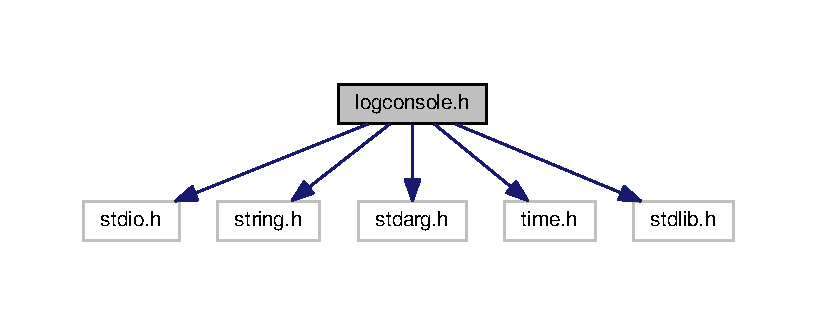
\includegraphics[width=350pt]{logconsole_8h__incl}
\end{center}
\end{figure}
This graph shows which files directly or indirectly include this file\+:\nopagebreak
\begin{figure}[H]
\begin{center}
\leavevmode
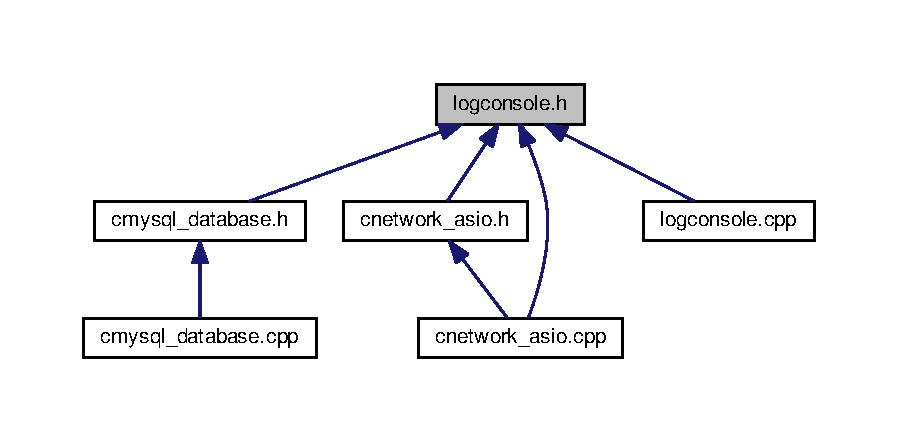
\includegraphics[width=350pt]{logconsole_8h__dep__incl}
\end{center}
\end{figure}
\subsection*{Classes}
\begin{DoxyCompactItemize}
\item 
class \hyperlink{classCore_1_1CLogConsole}{Core\+::\+C\+Log\+Console}
\end{DoxyCompactItemize}
\subsection*{Namespaces}
\begin{DoxyCompactItemize}
\item 
 \hyperlink{namespaceCore}{Core}
\end{DoxyCompactItemize}
\subsection*{Macros}
\begin{DoxyCompactItemize}
\item 
\#define \hyperlink{logconsole_8h_a2b041f826a6fbf53f7beb207ad910db0}{C\+L\+\_\+\+R\+E\+S\+ET}~\char`\"{}\textbackslash{}033\mbox{[}0m\char`\"{}
\item 
\#define \hyperlink{logconsole_8h_a12f884215934087f05e5eedd4980465c}{C\+L\+\_\+\+C\+LS}~\char`\"{}\textbackslash{}033\mbox{[}2\+J\char`\"{}
\item 
\#define \hyperlink{logconsole_8h_a226f0d2faed38cc2efe4274776dc3164}{C\+L\+\_\+\+C\+LL}~\char`\"{}\textbackslash{}033\mbox{[}K\char`\"{}
\item 
\#define \hyperlink{logconsole_8h_a7d3cf103d34eb3e590254f2008fc97ed}{C\+L\+\_\+\+B\+O\+LD}~\char`\"{}\textbackslash{}033\mbox{[}1m\char`\"{}
\item 
\#define \hyperlink{logconsole_8h_a20ded8b41f30e03ab9fb8a2c9792cbe3}{C\+L\+\_\+\+N\+O\+RM}~\hyperlink{logconsole_8h_a2b041f826a6fbf53f7beb207ad910db0}{C\+L\+\_\+\+R\+E\+S\+ET}
\item 
\#define \hyperlink{logconsole_8h_a3c9d41bc92627c550d90241d4476fa45}{C\+L\+\_\+\+N\+O\+R\+M\+AL}~\hyperlink{logconsole_8h_a2b041f826a6fbf53f7beb207ad910db0}{C\+L\+\_\+\+R\+E\+S\+ET}
\item 
\#define \hyperlink{logconsole_8h_a2e11831472bf30d5a2d5f7f62e49f43f}{C\+L\+\_\+\+N\+O\+NE}~\hyperlink{logconsole_8h_a2b041f826a6fbf53f7beb207ad910db0}{C\+L\+\_\+\+R\+E\+S\+ET}
\item 
\#define \hyperlink{logconsole_8h_a4a76a8255afca294a718979c77cbb12d}{C\+L\+\_\+\+W\+H\+I\+TE}~\char`\"{}\textbackslash{}033\mbox{[}1;37m\char`\"{}
\item 
\#define \hyperlink{logconsole_8h_a866292523a89df87461325bb58ce5c8b}{C\+L\+\_\+\+G\+R\+AY}~\char`\"{}\textbackslash{}033\mbox{[}1;30m\char`\"{}
\item 
\#define \hyperlink{logconsole_8h_a0d82cdd8a3e954be9701706dd21f98ae}{C\+L\+\_\+\+R\+ED}~\char`\"{}\textbackslash{}033\mbox{[}1;31m\char`\"{}
\item 
\#define \hyperlink{logconsole_8h_a2790ad32584d45e4a673776d95640c5a}{C\+L\+\_\+\+G\+R\+E\+EN}~\char`\"{}\textbackslash{}033\mbox{[}1;32m\char`\"{}
\item 
\#define \hyperlink{logconsole_8h_a995bf5374bbeba3fc4459d6a2b75ec75}{C\+L\+\_\+\+Y\+E\+L\+L\+OW}~\char`\"{}\textbackslash{}033\mbox{[}1;33m\char`\"{}
\item 
\#define \hyperlink{logconsole_8h_a4fa257b3b560f5bbd95332cb90cada05}{C\+L\+\_\+\+B\+L\+UE}~\char`\"{}\textbackslash{}033\mbox{[}1;34m\char`\"{}
\item 
\#define \hyperlink{logconsole_8h_a243acc41b506d2ec7b49672b4fcdbcfc}{C\+L\+\_\+\+M\+A\+G\+E\+N\+TA}~\char`\"{}\textbackslash{}033\mbox{[}1;35m\char`\"{}
\item 
\#define \hyperlink{logconsole_8h_a5c8e3046139550ceaea05f6f11ff6f95}{C\+L\+\_\+\+C\+Y\+AN}~\char`\"{}\textbackslash{}033\mbox{[}1;36m\char`\"{}
\item 
\#define \hyperlink{logconsole_8h_ab4ab50528360eade26594b7c9f6aad52}{C\+L\+\_\+\+B\+G\+\_\+\+B\+L\+A\+CK}~\char`\"{}\textbackslash{}033\mbox{[}40m\char`\"{}
\item 
\#define \hyperlink{logconsole_8h_aec38679d8f9d706e7e6e42173fac9679}{C\+L\+\_\+\+B\+G\+\_\+\+R\+ED}~\char`\"{}\textbackslash{}033\mbox{[}41m\char`\"{}
\item 
\#define \hyperlink{logconsole_8h_a87a7068f22a03e115e4de22728381858}{C\+L\+\_\+\+B\+G\+\_\+\+G\+R\+E\+EN}~\char`\"{}\textbackslash{}033\mbox{[}42m\char`\"{}
\item 
\#define \hyperlink{logconsole_8h_ad90531cec34a455960087ddee705064e}{C\+L\+\_\+\+B\+G\+\_\+\+Y\+E\+L\+L\+OW}~\char`\"{}\textbackslash{}033\mbox{[}43m\char`\"{}
\item 
\#define \hyperlink{logconsole_8h_abdcbc2a2e6d9a083c1e06972f97f9e54}{C\+L\+\_\+\+B\+G\+\_\+\+B\+L\+UE}~\char`\"{}\textbackslash{}033\mbox{[}44m\char`\"{}
\item 
\#define \hyperlink{logconsole_8h_aaa63e61ea6432c9d7fc23653064bd6a1}{C\+L\+\_\+\+B\+G\+\_\+\+M\+A\+G\+E\+N\+TA}~\char`\"{}\textbackslash{}033\mbox{[}45m\char`\"{}
\item 
\#define \hyperlink{logconsole_8h_a9a763050339065b6e126553c4f91a50f}{C\+L\+\_\+\+B\+G\+\_\+\+C\+Y\+AN}~\char`\"{}\textbackslash{}033\mbox{[}46m\char`\"{}
\item 
\#define \hyperlink{logconsole_8h_affdee4de2540d069abf6463b23512a2d}{C\+L\+\_\+\+B\+G\+\_\+\+W\+H\+I\+TE}~\char`\"{}\textbackslash{}033\mbox{[}47m\char`\"{}
\item 
\#define \hyperlink{logconsole_8h_a0d28404df238ba86073c508485380781}{C\+L\+\_\+\+L\+T\+\_\+\+B\+L\+A\+CK}~\char`\"{}\textbackslash{}033\mbox{[}0;30m\char`\"{}
\item 
\#define \hyperlink{logconsole_8h_ac7fc0860bf9fae8f4adb5cbece0d235b}{C\+L\+\_\+\+L\+T\+\_\+\+R\+ED}~\char`\"{}\textbackslash{}033\mbox{[}0;31m\char`\"{}
\item 
\#define \hyperlink{logconsole_8h_acdd052d49c25f0b8a56e6c85ea3f7661}{C\+L\+\_\+\+L\+T\+\_\+\+G\+R\+E\+EN}~\char`\"{}\textbackslash{}033\mbox{[}0;32m\char`\"{}
\item 
\#define \hyperlink{logconsole_8h_a84cb63ebd470b7eadeac0d181dbab274}{C\+L\+\_\+\+L\+T\+\_\+\+Y\+E\+L\+L\+OW}~\char`\"{}\textbackslash{}033\mbox{[}0;33m\char`\"{}
\item 
\#define \hyperlink{logconsole_8h_ae5b9ed83cdc10031794dc145a31da9ae}{C\+L\+\_\+\+L\+T\+\_\+\+B\+L\+UE}~\char`\"{}\textbackslash{}033\mbox{[}0;34m\char`\"{}
\item 
\#define \hyperlink{logconsole_8h_a31533a46f94ea1a4ccedc730071b5e32}{C\+L\+\_\+\+L\+T\+\_\+\+M\+A\+G\+E\+N\+TA}~\char`\"{}\textbackslash{}033\mbox{[}0;35m\char`\"{}
\item 
\#define \hyperlink{logconsole_8h_a94a87376126d22565b593cb8c0fe4da1}{C\+L\+\_\+\+L\+T\+\_\+\+C\+Y\+AN}~\char`\"{}\textbackslash{}033\mbox{[}0;36m\char`\"{}
\item 
\#define \hyperlink{logconsole_8h_ac36dda153f1f78ca152a4dcfef9f68cb}{C\+L\+\_\+\+L\+T\+\_\+\+W\+H\+I\+TE}~\char`\"{}\textbackslash{}033\mbox{[}0;37m\char`\"{}
\item 
\#define \hyperlink{logconsole_8h_a5496387d557f549fb0357c407570de25}{C\+L\+\_\+\+B\+T\+\_\+\+B\+L\+A\+CK}~\char`\"{}\textbackslash{}033\mbox{[}1;30m\char`\"{}
\item 
\#define \hyperlink{logconsole_8h_a6809d18e2fa89cc44e04ee5f86ca9b85}{C\+L\+\_\+\+B\+T\+\_\+\+R\+ED}~\char`\"{}\textbackslash{}033\mbox{[}1;31m\char`\"{}
\item 
\#define \hyperlink{logconsole_8h_a75963fba23e89b9c247dfbc96393e1e1}{C\+L\+\_\+\+B\+T\+\_\+\+G\+R\+E\+EN}~\char`\"{}\textbackslash{}033\mbox{[}1;32m\char`\"{}
\item 
\#define \hyperlink{logconsole_8h_a635c71f9d2b2e36c9ff67adc18f04f82}{C\+L\+\_\+\+B\+T\+\_\+\+Y\+E\+L\+L\+OW}~\char`\"{}\textbackslash{}033\mbox{[}1;33m\char`\"{}
\item 
\#define \hyperlink{logconsole_8h_a831772e3da9abda908fc6aa184762992}{C\+L\+\_\+\+B\+T\+\_\+\+B\+L\+UE}~\char`\"{}\textbackslash{}033\mbox{[}1;34m\char`\"{}
\item 
\#define \hyperlink{logconsole_8h_a72d8c54240772429429f7ae84cf242aa}{C\+L\+\_\+\+B\+T\+\_\+\+M\+A\+G\+E\+N\+TA}~\char`\"{}\textbackslash{}033\mbox{[}1;35m\char`\"{}
\item 
\#define \hyperlink{logconsole_8h_a18435d8c74415b9be4da13b4d65fffe8}{C\+L\+\_\+\+B\+T\+\_\+\+C\+Y\+AN}~\char`\"{}\textbackslash{}033\mbox{[}1;36m\char`\"{}
\item 
\#define \hyperlink{logconsole_8h_ac97c18c4f25fa23aa57e249f2e7292c7}{C\+L\+\_\+\+B\+T\+\_\+\+W\+H\+I\+TE}~\char`\"{}\textbackslash{}033\mbox{[}1;37m\char`\"{}
\end{DoxyCompactItemize}
\subsection*{Functions}
\begin{DoxyCompactItemize}
\item 
int \hyperlink{namespaceCore_ac841f812f5ff61ba38222f7d441509d3}{Core\+::clprintf} (const char $\ast$fmt,...)
\item 
int \hyperlink{namespaceCore_a630dcb213704b7856eec935d8695ffe9}{Core\+::clvprintf} (const char $\ast$fmt, va\+\_\+list)
\end{DoxyCompactItemize}


\subsection{Macro Definition Documentation}
\index{logconsole.\+h@{logconsole.\+h}!C\+L\+\_\+\+B\+G\+\_\+\+B\+L\+A\+CK@{C\+L\+\_\+\+B\+G\+\_\+\+B\+L\+A\+CK}}
\index{C\+L\+\_\+\+B\+G\+\_\+\+B\+L\+A\+CK@{C\+L\+\_\+\+B\+G\+\_\+\+B\+L\+A\+CK}!logconsole.\+h@{logconsole.\+h}}
\subsubsection[{\texorpdfstring{C\+L\+\_\+\+B\+G\+\_\+\+B\+L\+A\+CK}{CL_BG_BLACK}}]{\setlength{\rightskip}{0pt plus 5cm}\#define C\+L\+\_\+\+B\+G\+\_\+\+B\+L\+A\+CK~\char`\"{}\textbackslash{}033\mbox{[}40m\char`\"{}}\hypertarget{logconsole_8h_ab4ab50528360eade26594b7c9f6aad52}{}\label{logconsole_8h_ab4ab50528360eade26594b7c9f6aad52}
\index{logconsole.\+h@{logconsole.\+h}!C\+L\+\_\+\+B\+G\+\_\+\+B\+L\+UE@{C\+L\+\_\+\+B\+G\+\_\+\+B\+L\+UE}}
\index{C\+L\+\_\+\+B\+G\+\_\+\+B\+L\+UE@{C\+L\+\_\+\+B\+G\+\_\+\+B\+L\+UE}!logconsole.\+h@{logconsole.\+h}}
\subsubsection[{\texorpdfstring{C\+L\+\_\+\+B\+G\+\_\+\+B\+L\+UE}{CL_BG_BLUE}}]{\setlength{\rightskip}{0pt plus 5cm}\#define C\+L\+\_\+\+B\+G\+\_\+\+B\+L\+UE~\char`\"{}\textbackslash{}033\mbox{[}44m\char`\"{}}\hypertarget{logconsole_8h_abdcbc2a2e6d9a083c1e06972f97f9e54}{}\label{logconsole_8h_abdcbc2a2e6d9a083c1e06972f97f9e54}
\index{logconsole.\+h@{logconsole.\+h}!C\+L\+\_\+\+B\+G\+\_\+\+C\+Y\+AN@{C\+L\+\_\+\+B\+G\+\_\+\+C\+Y\+AN}}
\index{C\+L\+\_\+\+B\+G\+\_\+\+C\+Y\+AN@{C\+L\+\_\+\+B\+G\+\_\+\+C\+Y\+AN}!logconsole.\+h@{logconsole.\+h}}
\subsubsection[{\texorpdfstring{C\+L\+\_\+\+B\+G\+\_\+\+C\+Y\+AN}{CL_BG_CYAN}}]{\setlength{\rightskip}{0pt plus 5cm}\#define C\+L\+\_\+\+B\+G\+\_\+\+C\+Y\+AN~\char`\"{}\textbackslash{}033\mbox{[}46m\char`\"{}}\hypertarget{logconsole_8h_a9a763050339065b6e126553c4f91a50f}{}\label{logconsole_8h_a9a763050339065b6e126553c4f91a50f}
\index{logconsole.\+h@{logconsole.\+h}!C\+L\+\_\+\+B\+G\+\_\+\+G\+R\+E\+EN@{C\+L\+\_\+\+B\+G\+\_\+\+G\+R\+E\+EN}}
\index{C\+L\+\_\+\+B\+G\+\_\+\+G\+R\+E\+EN@{C\+L\+\_\+\+B\+G\+\_\+\+G\+R\+E\+EN}!logconsole.\+h@{logconsole.\+h}}
\subsubsection[{\texorpdfstring{C\+L\+\_\+\+B\+G\+\_\+\+G\+R\+E\+EN}{CL_BG_GREEN}}]{\setlength{\rightskip}{0pt plus 5cm}\#define C\+L\+\_\+\+B\+G\+\_\+\+G\+R\+E\+EN~\char`\"{}\textbackslash{}033\mbox{[}42m\char`\"{}}\hypertarget{logconsole_8h_a87a7068f22a03e115e4de22728381858}{}\label{logconsole_8h_a87a7068f22a03e115e4de22728381858}
\index{logconsole.\+h@{logconsole.\+h}!C\+L\+\_\+\+B\+G\+\_\+\+M\+A\+G\+E\+N\+TA@{C\+L\+\_\+\+B\+G\+\_\+\+M\+A\+G\+E\+N\+TA}}
\index{C\+L\+\_\+\+B\+G\+\_\+\+M\+A\+G\+E\+N\+TA@{C\+L\+\_\+\+B\+G\+\_\+\+M\+A\+G\+E\+N\+TA}!logconsole.\+h@{logconsole.\+h}}
\subsubsection[{\texorpdfstring{C\+L\+\_\+\+B\+G\+\_\+\+M\+A\+G\+E\+N\+TA}{CL_BG_MAGENTA}}]{\setlength{\rightskip}{0pt plus 5cm}\#define C\+L\+\_\+\+B\+G\+\_\+\+M\+A\+G\+E\+N\+TA~\char`\"{}\textbackslash{}033\mbox{[}45m\char`\"{}}\hypertarget{logconsole_8h_aaa63e61ea6432c9d7fc23653064bd6a1}{}\label{logconsole_8h_aaa63e61ea6432c9d7fc23653064bd6a1}
\index{logconsole.\+h@{logconsole.\+h}!C\+L\+\_\+\+B\+G\+\_\+\+R\+ED@{C\+L\+\_\+\+B\+G\+\_\+\+R\+ED}}
\index{C\+L\+\_\+\+B\+G\+\_\+\+R\+ED@{C\+L\+\_\+\+B\+G\+\_\+\+R\+ED}!logconsole.\+h@{logconsole.\+h}}
\subsubsection[{\texorpdfstring{C\+L\+\_\+\+B\+G\+\_\+\+R\+ED}{CL_BG_RED}}]{\setlength{\rightskip}{0pt plus 5cm}\#define C\+L\+\_\+\+B\+G\+\_\+\+R\+ED~\char`\"{}\textbackslash{}033\mbox{[}41m\char`\"{}}\hypertarget{logconsole_8h_aec38679d8f9d706e7e6e42173fac9679}{}\label{logconsole_8h_aec38679d8f9d706e7e6e42173fac9679}
\index{logconsole.\+h@{logconsole.\+h}!C\+L\+\_\+\+B\+G\+\_\+\+W\+H\+I\+TE@{C\+L\+\_\+\+B\+G\+\_\+\+W\+H\+I\+TE}}
\index{C\+L\+\_\+\+B\+G\+\_\+\+W\+H\+I\+TE@{C\+L\+\_\+\+B\+G\+\_\+\+W\+H\+I\+TE}!logconsole.\+h@{logconsole.\+h}}
\subsubsection[{\texorpdfstring{C\+L\+\_\+\+B\+G\+\_\+\+W\+H\+I\+TE}{CL_BG_WHITE}}]{\setlength{\rightskip}{0pt plus 5cm}\#define C\+L\+\_\+\+B\+G\+\_\+\+W\+H\+I\+TE~\char`\"{}\textbackslash{}033\mbox{[}47m\char`\"{}}\hypertarget{logconsole_8h_affdee4de2540d069abf6463b23512a2d}{}\label{logconsole_8h_affdee4de2540d069abf6463b23512a2d}
\index{logconsole.\+h@{logconsole.\+h}!C\+L\+\_\+\+B\+G\+\_\+\+Y\+E\+L\+L\+OW@{C\+L\+\_\+\+B\+G\+\_\+\+Y\+E\+L\+L\+OW}}
\index{C\+L\+\_\+\+B\+G\+\_\+\+Y\+E\+L\+L\+OW@{C\+L\+\_\+\+B\+G\+\_\+\+Y\+E\+L\+L\+OW}!logconsole.\+h@{logconsole.\+h}}
\subsubsection[{\texorpdfstring{C\+L\+\_\+\+B\+G\+\_\+\+Y\+E\+L\+L\+OW}{CL_BG_YELLOW}}]{\setlength{\rightskip}{0pt plus 5cm}\#define C\+L\+\_\+\+B\+G\+\_\+\+Y\+E\+L\+L\+OW~\char`\"{}\textbackslash{}033\mbox{[}43m\char`\"{}}\hypertarget{logconsole_8h_ad90531cec34a455960087ddee705064e}{}\label{logconsole_8h_ad90531cec34a455960087ddee705064e}
\index{logconsole.\+h@{logconsole.\+h}!C\+L\+\_\+\+B\+L\+UE@{C\+L\+\_\+\+B\+L\+UE}}
\index{C\+L\+\_\+\+B\+L\+UE@{C\+L\+\_\+\+B\+L\+UE}!logconsole.\+h@{logconsole.\+h}}
\subsubsection[{\texorpdfstring{C\+L\+\_\+\+B\+L\+UE}{CL_BLUE}}]{\setlength{\rightskip}{0pt plus 5cm}\#define C\+L\+\_\+\+B\+L\+UE~\char`\"{}\textbackslash{}033\mbox{[}1;34m\char`\"{}}\hypertarget{logconsole_8h_a4fa257b3b560f5bbd95332cb90cada05}{}\label{logconsole_8h_a4fa257b3b560f5bbd95332cb90cada05}
\index{logconsole.\+h@{logconsole.\+h}!C\+L\+\_\+\+B\+O\+LD@{C\+L\+\_\+\+B\+O\+LD}}
\index{C\+L\+\_\+\+B\+O\+LD@{C\+L\+\_\+\+B\+O\+LD}!logconsole.\+h@{logconsole.\+h}}
\subsubsection[{\texorpdfstring{C\+L\+\_\+\+B\+O\+LD}{CL_BOLD}}]{\setlength{\rightskip}{0pt plus 5cm}\#define C\+L\+\_\+\+B\+O\+LD~\char`\"{}\textbackslash{}033\mbox{[}1m\char`\"{}}\hypertarget{logconsole_8h_a7d3cf103d34eb3e590254f2008fc97ed}{}\label{logconsole_8h_a7d3cf103d34eb3e590254f2008fc97ed}
\index{logconsole.\+h@{logconsole.\+h}!C\+L\+\_\+\+B\+T\+\_\+\+B\+L\+A\+CK@{C\+L\+\_\+\+B\+T\+\_\+\+B\+L\+A\+CK}}
\index{C\+L\+\_\+\+B\+T\+\_\+\+B\+L\+A\+CK@{C\+L\+\_\+\+B\+T\+\_\+\+B\+L\+A\+CK}!logconsole.\+h@{logconsole.\+h}}
\subsubsection[{\texorpdfstring{C\+L\+\_\+\+B\+T\+\_\+\+B\+L\+A\+CK}{CL_BT_BLACK}}]{\setlength{\rightskip}{0pt plus 5cm}\#define C\+L\+\_\+\+B\+T\+\_\+\+B\+L\+A\+CK~\char`\"{}\textbackslash{}033\mbox{[}1;30m\char`\"{}}\hypertarget{logconsole_8h_a5496387d557f549fb0357c407570de25}{}\label{logconsole_8h_a5496387d557f549fb0357c407570de25}
\index{logconsole.\+h@{logconsole.\+h}!C\+L\+\_\+\+B\+T\+\_\+\+B\+L\+UE@{C\+L\+\_\+\+B\+T\+\_\+\+B\+L\+UE}}
\index{C\+L\+\_\+\+B\+T\+\_\+\+B\+L\+UE@{C\+L\+\_\+\+B\+T\+\_\+\+B\+L\+UE}!logconsole.\+h@{logconsole.\+h}}
\subsubsection[{\texorpdfstring{C\+L\+\_\+\+B\+T\+\_\+\+B\+L\+UE}{CL_BT_BLUE}}]{\setlength{\rightskip}{0pt plus 5cm}\#define C\+L\+\_\+\+B\+T\+\_\+\+B\+L\+UE~\char`\"{}\textbackslash{}033\mbox{[}1;34m\char`\"{}}\hypertarget{logconsole_8h_a831772e3da9abda908fc6aa184762992}{}\label{logconsole_8h_a831772e3da9abda908fc6aa184762992}
\index{logconsole.\+h@{logconsole.\+h}!C\+L\+\_\+\+B\+T\+\_\+\+C\+Y\+AN@{C\+L\+\_\+\+B\+T\+\_\+\+C\+Y\+AN}}
\index{C\+L\+\_\+\+B\+T\+\_\+\+C\+Y\+AN@{C\+L\+\_\+\+B\+T\+\_\+\+C\+Y\+AN}!logconsole.\+h@{logconsole.\+h}}
\subsubsection[{\texorpdfstring{C\+L\+\_\+\+B\+T\+\_\+\+C\+Y\+AN}{CL_BT_CYAN}}]{\setlength{\rightskip}{0pt plus 5cm}\#define C\+L\+\_\+\+B\+T\+\_\+\+C\+Y\+AN~\char`\"{}\textbackslash{}033\mbox{[}1;36m\char`\"{}}\hypertarget{logconsole_8h_a18435d8c74415b9be4da13b4d65fffe8}{}\label{logconsole_8h_a18435d8c74415b9be4da13b4d65fffe8}
\index{logconsole.\+h@{logconsole.\+h}!C\+L\+\_\+\+B\+T\+\_\+\+G\+R\+E\+EN@{C\+L\+\_\+\+B\+T\+\_\+\+G\+R\+E\+EN}}
\index{C\+L\+\_\+\+B\+T\+\_\+\+G\+R\+E\+EN@{C\+L\+\_\+\+B\+T\+\_\+\+G\+R\+E\+EN}!logconsole.\+h@{logconsole.\+h}}
\subsubsection[{\texorpdfstring{C\+L\+\_\+\+B\+T\+\_\+\+G\+R\+E\+EN}{CL_BT_GREEN}}]{\setlength{\rightskip}{0pt plus 5cm}\#define C\+L\+\_\+\+B\+T\+\_\+\+G\+R\+E\+EN~\char`\"{}\textbackslash{}033\mbox{[}1;32m\char`\"{}}\hypertarget{logconsole_8h_a75963fba23e89b9c247dfbc96393e1e1}{}\label{logconsole_8h_a75963fba23e89b9c247dfbc96393e1e1}
\index{logconsole.\+h@{logconsole.\+h}!C\+L\+\_\+\+B\+T\+\_\+\+M\+A\+G\+E\+N\+TA@{C\+L\+\_\+\+B\+T\+\_\+\+M\+A\+G\+E\+N\+TA}}
\index{C\+L\+\_\+\+B\+T\+\_\+\+M\+A\+G\+E\+N\+TA@{C\+L\+\_\+\+B\+T\+\_\+\+M\+A\+G\+E\+N\+TA}!logconsole.\+h@{logconsole.\+h}}
\subsubsection[{\texorpdfstring{C\+L\+\_\+\+B\+T\+\_\+\+M\+A\+G\+E\+N\+TA}{CL_BT_MAGENTA}}]{\setlength{\rightskip}{0pt plus 5cm}\#define C\+L\+\_\+\+B\+T\+\_\+\+M\+A\+G\+E\+N\+TA~\char`\"{}\textbackslash{}033\mbox{[}1;35m\char`\"{}}\hypertarget{logconsole_8h_a72d8c54240772429429f7ae84cf242aa}{}\label{logconsole_8h_a72d8c54240772429429f7ae84cf242aa}
\index{logconsole.\+h@{logconsole.\+h}!C\+L\+\_\+\+B\+T\+\_\+\+R\+ED@{C\+L\+\_\+\+B\+T\+\_\+\+R\+ED}}
\index{C\+L\+\_\+\+B\+T\+\_\+\+R\+ED@{C\+L\+\_\+\+B\+T\+\_\+\+R\+ED}!logconsole.\+h@{logconsole.\+h}}
\subsubsection[{\texorpdfstring{C\+L\+\_\+\+B\+T\+\_\+\+R\+ED}{CL_BT_RED}}]{\setlength{\rightskip}{0pt plus 5cm}\#define C\+L\+\_\+\+B\+T\+\_\+\+R\+ED~\char`\"{}\textbackslash{}033\mbox{[}1;31m\char`\"{}}\hypertarget{logconsole_8h_a6809d18e2fa89cc44e04ee5f86ca9b85}{}\label{logconsole_8h_a6809d18e2fa89cc44e04ee5f86ca9b85}
\index{logconsole.\+h@{logconsole.\+h}!C\+L\+\_\+\+B\+T\+\_\+\+W\+H\+I\+TE@{C\+L\+\_\+\+B\+T\+\_\+\+W\+H\+I\+TE}}
\index{C\+L\+\_\+\+B\+T\+\_\+\+W\+H\+I\+TE@{C\+L\+\_\+\+B\+T\+\_\+\+W\+H\+I\+TE}!logconsole.\+h@{logconsole.\+h}}
\subsubsection[{\texorpdfstring{C\+L\+\_\+\+B\+T\+\_\+\+W\+H\+I\+TE}{CL_BT_WHITE}}]{\setlength{\rightskip}{0pt plus 5cm}\#define C\+L\+\_\+\+B\+T\+\_\+\+W\+H\+I\+TE~\char`\"{}\textbackslash{}033\mbox{[}1;37m\char`\"{}}\hypertarget{logconsole_8h_ac97c18c4f25fa23aa57e249f2e7292c7}{}\label{logconsole_8h_ac97c18c4f25fa23aa57e249f2e7292c7}
\index{logconsole.\+h@{logconsole.\+h}!C\+L\+\_\+\+B\+T\+\_\+\+Y\+E\+L\+L\+OW@{C\+L\+\_\+\+B\+T\+\_\+\+Y\+E\+L\+L\+OW}}
\index{C\+L\+\_\+\+B\+T\+\_\+\+Y\+E\+L\+L\+OW@{C\+L\+\_\+\+B\+T\+\_\+\+Y\+E\+L\+L\+OW}!logconsole.\+h@{logconsole.\+h}}
\subsubsection[{\texorpdfstring{C\+L\+\_\+\+B\+T\+\_\+\+Y\+E\+L\+L\+OW}{CL_BT_YELLOW}}]{\setlength{\rightskip}{0pt plus 5cm}\#define C\+L\+\_\+\+B\+T\+\_\+\+Y\+E\+L\+L\+OW~\char`\"{}\textbackslash{}033\mbox{[}1;33m\char`\"{}}\hypertarget{logconsole_8h_a635c71f9d2b2e36c9ff67adc18f04f82}{}\label{logconsole_8h_a635c71f9d2b2e36c9ff67adc18f04f82}
\index{logconsole.\+h@{logconsole.\+h}!C\+L\+\_\+\+C\+LL@{C\+L\+\_\+\+C\+LL}}
\index{C\+L\+\_\+\+C\+LL@{C\+L\+\_\+\+C\+LL}!logconsole.\+h@{logconsole.\+h}}
\subsubsection[{\texorpdfstring{C\+L\+\_\+\+C\+LL}{CL_CLL}}]{\setlength{\rightskip}{0pt plus 5cm}\#define C\+L\+\_\+\+C\+LL~\char`\"{}\textbackslash{}033\mbox{[}K\char`\"{}}\hypertarget{logconsole_8h_a226f0d2faed38cc2efe4274776dc3164}{}\label{logconsole_8h_a226f0d2faed38cc2efe4274776dc3164}
\index{logconsole.\+h@{logconsole.\+h}!C\+L\+\_\+\+C\+LS@{C\+L\+\_\+\+C\+LS}}
\index{C\+L\+\_\+\+C\+LS@{C\+L\+\_\+\+C\+LS}!logconsole.\+h@{logconsole.\+h}}
\subsubsection[{\texorpdfstring{C\+L\+\_\+\+C\+LS}{CL_CLS}}]{\setlength{\rightskip}{0pt plus 5cm}\#define C\+L\+\_\+\+C\+LS~\char`\"{}\textbackslash{}033\mbox{[}2\+J\char`\"{}}\hypertarget{logconsole_8h_a12f884215934087f05e5eedd4980465c}{}\label{logconsole_8h_a12f884215934087f05e5eedd4980465c}
\index{logconsole.\+h@{logconsole.\+h}!C\+L\+\_\+\+C\+Y\+AN@{C\+L\+\_\+\+C\+Y\+AN}}
\index{C\+L\+\_\+\+C\+Y\+AN@{C\+L\+\_\+\+C\+Y\+AN}!logconsole.\+h@{logconsole.\+h}}
\subsubsection[{\texorpdfstring{C\+L\+\_\+\+C\+Y\+AN}{CL_CYAN}}]{\setlength{\rightskip}{0pt plus 5cm}\#define C\+L\+\_\+\+C\+Y\+AN~\char`\"{}\textbackslash{}033\mbox{[}1;36m\char`\"{}}\hypertarget{logconsole_8h_a5c8e3046139550ceaea05f6f11ff6f95}{}\label{logconsole_8h_a5c8e3046139550ceaea05f6f11ff6f95}
\index{logconsole.\+h@{logconsole.\+h}!C\+L\+\_\+\+G\+R\+AY@{C\+L\+\_\+\+G\+R\+AY}}
\index{C\+L\+\_\+\+G\+R\+AY@{C\+L\+\_\+\+G\+R\+AY}!logconsole.\+h@{logconsole.\+h}}
\subsubsection[{\texorpdfstring{C\+L\+\_\+\+G\+R\+AY}{CL_GRAY}}]{\setlength{\rightskip}{0pt plus 5cm}\#define C\+L\+\_\+\+G\+R\+AY~\char`\"{}\textbackslash{}033\mbox{[}1;30m\char`\"{}}\hypertarget{logconsole_8h_a866292523a89df87461325bb58ce5c8b}{}\label{logconsole_8h_a866292523a89df87461325bb58ce5c8b}
\index{logconsole.\+h@{logconsole.\+h}!C\+L\+\_\+\+G\+R\+E\+EN@{C\+L\+\_\+\+G\+R\+E\+EN}}
\index{C\+L\+\_\+\+G\+R\+E\+EN@{C\+L\+\_\+\+G\+R\+E\+EN}!logconsole.\+h@{logconsole.\+h}}
\subsubsection[{\texorpdfstring{C\+L\+\_\+\+G\+R\+E\+EN}{CL_GREEN}}]{\setlength{\rightskip}{0pt plus 5cm}\#define C\+L\+\_\+\+G\+R\+E\+EN~\char`\"{}\textbackslash{}033\mbox{[}1;32m\char`\"{}}\hypertarget{logconsole_8h_a2790ad32584d45e4a673776d95640c5a}{}\label{logconsole_8h_a2790ad32584d45e4a673776d95640c5a}
\index{logconsole.\+h@{logconsole.\+h}!C\+L\+\_\+\+L\+T\+\_\+\+B\+L\+A\+CK@{C\+L\+\_\+\+L\+T\+\_\+\+B\+L\+A\+CK}}
\index{C\+L\+\_\+\+L\+T\+\_\+\+B\+L\+A\+CK@{C\+L\+\_\+\+L\+T\+\_\+\+B\+L\+A\+CK}!logconsole.\+h@{logconsole.\+h}}
\subsubsection[{\texorpdfstring{C\+L\+\_\+\+L\+T\+\_\+\+B\+L\+A\+CK}{CL_LT_BLACK}}]{\setlength{\rightskip}{0pt plus 5cm}\#define C\+L\+\_\+\+L\+T\+\_\+\+B\+L\+A\+CK~\char`\"{}\textbackslash{}033\mbox{[}0;30m\char`\"{}}\hypertarget{logconsole_8h_a0d28404df238ba86073c508485380781}{}\label{logconsole_8h_a0d28404df238ba86073c508485380781}
\index{logconsole.\+h@{logconsole.\+h}!C\+L\+\_\+\+L\+T\+\_\+\+B\+L\+UE@{C\+L\+\_\+\+L\+T\+\_\+\+B\+L\+UE}}
\index{C\+L\+\_\+\+L\+T\+\_\+\+B\+L\+UE@{C\+L\+\_\+\+L\+T\+\_\+\+B\+L\+UE}!logconsole.\+h@{logconsole.\+h}}
\subsubsection[{\texorpdfstring{C\+L\+\_\+\+L\+T\+\_\+\+B\+L\+UE}{CL_LT_BLUE}}]{\setlength{\rightskip}{0pt plus 5cm}\#define C\+L\+\_\+\+L\+T\+\_\+\+B\+L\+UE~\char`\"{}\textbackslash{}033\mbox{[}0;34m\char`\"{}}\hypertarget{logconsole_8h_ae5b9ed83cdc10031794dc145a31da9ae}{}\label{logconsole_8h_ae5b9ed83cdc10031794dc145a31da9ae}
\index{logconsole.\+h@{logconsole.\+h}!C\+L\+\_\+\+L\+T\+\_\+\+C\+Y\+AN@{C\+L\+\_\+\+L\+T\+\_\+\+C\+Y\+AN}}
\index{C\+L\+\_\+\+L\+T\+\_\+\+C\+Y\+AN@{C\+L\+\_\+\+L\+T\+\_\+\+C\+Y\+AN}!logconsole.\+h@{logconsole.\+h}}
\subsubsection[{\texorpdfstring{C\+L\+\_\+\+L\+T\+\_\+\+C\+Y\+AN}{CL_LT_CYAN}}]{\setlength{\rightskip}{0pt plus 5cm}\#define C\+L\+\_\+\+L\+T\+\_\+\+C\+Y\+AN~\char`\"{}\textbackslash{}033\mbox{[}0;36m\char`\"{}}\hypertarget{logconsole_8h_a94a87376126d22565b593cb8c0fe4da1}{}\label{logconsole_8h_a94a87376126d22565b593cb8c0fe4da1}
\index{logconsole.\+h@{logconsole.\+h}!C\+L\+\_\+\+L\+T\+\_\+\+G\+R\+E\+EN@{C\+L\+\_\+\+L\+T\+\_\+\+G\+R\+E\+EN}}
\index{C\+L\+\_\+\+L\+T\+\_\+\+G\+R\+E\+EN@{C\+L\+\_\+\+L\+T\+\_\+\+G\+R\+E\+EN}!logconsole.\+h@{logconsole.\+h}}
\subsubsection[{\texorpdfstring{C\+L\+\_\+\+L\+T\+\_\+\+G\+R\+E\+EN}{CL_LT_GREEN}}]{\setlength{\rightskip}{0pt plus 5cm}\#define C\+L\+\_\+\+L\+T\+\_\+\+G\+R\+E\+EN~\char`\"{}\textbackslash{}033\mbox{[}0;32m\char`\"{}}\hypertarget{logconsole_8h_acdd052d49c25f0b8a56e6c85ea3f7661}{}\label{logconsole_8h_acdd052d49c25f0b8a56e6c85ea3f7661}
\index{logconsole.\+h@{logconsole.\+h}!C\+L\+\_\+\+L\+T\+\_\+\+M\+A\+G\+E\+N\+TA@{C\+L\+\_\+\+L\+T\+\_\+\+M\+A\+G\+E\+N\+TA}}
\index{C\+L\+\_\+\+L\+T\+\_\+\+M\+A\+G\+E\+N\+TA@{C\+L\+\_\+\+L\+T\+\_\+\+M\+A\+G\+E\+N\+TA}!logconsole.\+h@{logconsole.\+h}}
\subsubsection[{\texorpdfstring{C\+L\+\_\+\+L\+T\+\_\+\+M\+A\+G\+E\+N\+TA}{CL_LT_MAGENTA}}]{\setlength{\rightskip}{0pt plus 5cm}\#define C\+L\+\_\+\+L\+T\+\_\+\+M\+A\+G\+E\+N\+TA~\char`\"{}\textbackslash{}033\mbox{[}0;35m\char`\"{}}\hypertarget{logconsole_8h_a31533a46f94ea1a4ccedc730071b5e32}{}\label{logconsole_8h_a31533a46f94ea1a4ccedc730071b5e32}
\index{logconsole.\+h@{logconsole.\+h}!C\+L\+\_\+\+L\+T\+\_\+\+R\+ED@{C\+L\+\_\+\+L\+T\+\_\+\+R\+ED}}
\index{C\+L\+\_\+\+L\+T\+\_\+\+R\+ED@{C\+L\+\_\+\+L\+T\+\_\+\+R\+ED}!logconsole.\+h@{logconsole.\+h}}
\subsubsection[{\texorpdfstring{C\+L\+\_\+\+L\+T\+\_\+\+R\+ED}{CL_LT_RED}}]{\setlength{\rightskip}{0pt plus 5cm}\#define C\+L\+\_\+\+L\+T\+\_\+\+R\+ED~\char`\"{}\textbackslash{}033\mbox{[}0;31m\char`\"{}}\hypertarget{logconsole_8h_ac7fc0860bf9fae8f4adb5cbece0d235b}{}\label{logconsole_8h_ac7fc0860bf9fae8f4adb5cbece0d235b}
\index{logconsole.\+h@{logconsole.\+h}!C\+L\+\_\+\+L\+T\+\_\+\+W\+H\+I\+TE@{C\+L\+\_\+\+L\+T\+\_\+\+W\+H\+I\+TE}}
\index{C\+L\+\_\+\+L\+T\+\_\+\+W\+H\+I\+TE@{C\+L\+\_\+\+L\+T\+\_\+\+W\+H\+I\+TE}!logconsole.\+h@{logconsole.\+h}}
\subsubsection[{\texorpdfstring{C\+L\+\_\+\+L\+T\+\_\+\+W\+H\+I\+TE}{CL_LT_WHITE}}]{\setlength{\rightskip}{0pt plus 5cm}\#define C\+L\+\_\+\+L\+T\+\_\+\+W\+H\+I\+TE~\char`\"{}\textbackslash{}033\mbox{[}0;37m\char`\"{}}\hypertarget{logconsole_8h_ac36dda153f1f78ca152a4dcfef9f68cb}{}\label{logconsole_8h_ac36dda153f1f78ca152a4dcfef9f68cb}
\index{logconsole.\+h@{logconsole.\+h}!C\+L\+\_\+\+L\+T\+\_\+\+Y\+E\+L\+L\+OW@{C\+L\+\_\+\+L\+T\+\_\+\+Y\+E\+L\+L\+OW}}
\index{C\+L\+\_\+\+L\+T\+\_\+\+Y\+E\+L\+L\+OW@{C\+L\+\_\+\+L\+T\+\_\+\+Y\+E\+L\+L\+OW}!logconsole.\+h@{logconsole.\+h}}
\subsubsection[{\texorpdfstring{C\+L\+\_\+\+L\+T\+\_\+\+Y\+E\+L\+L\+OW}{CL_LT_YELLOW}}]{\setlength{\rightskip}{0pt plus 5cm}\#define C\+L\+\_\+\+L\+T\+\_\+\+Y\+E\+L\+L\+OW~\char`\"{}\textbackslash{}033\mbox{[}0;33m\char`\"{}}\hypertarget{logconsole_8h_a84cb63ebd470b7eadeac0d181dbab274}{}\label{logconsole_8h_a84cb63ebd470b7eadeac0d181dbab274}
\index{logconsole.\+h@{logconsole.\+h}!C\+L\+\_\+\+M\+A\+G\+E\+N\+TA@{C\+L\+\_\+\+M\+A\+G\+E\+N\+TA}}
\index{C\+L\+\_\+\+M\+A\+G\+E\+N\+TA@{C\+L\+\_\+\+M\+A\+G\+E\+N\+TA}!logconsole.\+h@{logconsole.\+h}}
\subsubsection[{\texorpdfstring{C\+L\+\_\+\+M\+A\+G\+E\+N\+TA}{CL_MAGENTA}}]{\setlength{\rightskip}{0pt plus 5cm}\#define C\+L\+\_\+\+M\+A\+G\+E\+N\+TA~\char`\"{}\textbackslash{}033\mbox{[}1;35m\char`\"{}}\hypertarget{logconsole_8h_a243acc41b506d2ec7b49672b4fcdbcfc}{}\label{logconsole_8h_a243acc41b506d2ec7b49672b4fcdbcfc}
\index{logconsole.\+h@{logconsole.\+h}!C\+L\+\_\+\+N\+O\+NE@{C\+L\+\_\+\+N\+O\+NE}}
\index{C\+L\+\_\+\+N\+O\+NE@{C\+L\+\_\+\+N\+O\+NE}!logconsole.\+h@{logconsole.\+h}}
\subsubsection[{\texorpdfstring{C\+L\+\_\+\+N\+O\+NE}{CL_NONE}}]{\setlength{\rightskip}{0pt plus 5cm}\#define C\+L\+\_\+\+N\+O\+NE~{\bf C\+L\+\_\+\+R\+E\+S\+ET}}\hypertarget{logconsole_8h_a2e11831472bf30d5a2d5f7f62e49f43f}{}\label{logconsole_8h_a2e11831472bf30d5a2d5f7f62e49f43f}
\index{logconsole.\+h@{logconsole.\+h}!C\+L\+\_\+\+N\+O\+RM@{C\+L\+\_\+\+N\+O\+RM}}
\index{C\+L\+\_\+\+N\+O\+RM@{C\+L\+\_\+\+N\+O\+RM}!logconsole.\+h@{logconsole.\+h}}
\subsubsection[{\texorpdfstring{C\+L\+\_\+\+N\+O\+RM}{CL_NORM}}]{\setlength{\rightskip}{0pt plus 5cm}\#define C\+L\+\_\+\+N\+O\+RM~{\bf C\+L\+\_\+\+R\+E\+S\+ET}}\hypertarget{logconsole_8h_a20ded8b41f30e03ab9fb8a2c9792cbe3}{}\label{logconsole_8h_a20ded8b41f30e03ab9fb8a2c9792cbe3}
\index{logconsole.\+h@{logconsole.\+h}!C\+L\+\_\+\+N\+O\+R\+M\+AL@{C\+L\+\_\+\+N\+O\+R\+M\+AL}}
\index{C\+L\+\_\+\+N\+O\+R\+M\+AL@{C\+L\+\_\+\+N\+O\+R\+M\+AL}!logconsole.\+h@{logconsole.\+h}}
\subsubsection[{\texorpdfstring{C\+L\+\_\+\+N\+O\+R\+M\+AL}{CL_NORMAL}}]{\setlength{\rightskip}{0pt plus 5cm}\#define C\+L\+\_\+\+N\+O\+R\+M\+AL~{\bf C\+L\+\_\+\+R\+E\+S\+ET}}\hypertarget{logconsole_8h_a3c9d41bc92627c550d90241d4476fa45}{}\label{logconsole_8h_a3c9d41bc92627c550d90241d4476fa45}
\index{logconsole.\+h@{logconsole.\+h}!C\+L\+\_\+\+R\+ED@{C\+L\+\_\+\+R\+ED}}
\index{C\+L\+\_\+\+R\+ED@{C\+L\+\_\+\+R\+ED}!logconsole.\+h@{logconsole.\+h}}
\subsubsection[{\texorpdfstring{C\+L\+\_\+\+R\+ED}{CL_RED}}]{\setlength{\rightskip}{0pt plus 5cm}\#define C\+L\+\_\+\+R\+ED~\char`\"{}\textbackslash{}033\mbox{[}1;31m\char`\"{}}\hypertarget{logconsole_8h_a0d82cdd8a3e954be9701706dd21f98ae}{}\label{logconsole_8h_a0d82cdd8a3e954be9701706dd21f98ae}
\index{logconsole.\+h@{logconsole.\+h}!C\+L\+\_\+\+R\+E\+S\+ET@{C\+L\+\_\+\+R\+E\+S\+ET}}
\index{C\+L\+\_\+\+R\+E\+S\+ET@{C\+L\+\_\+\+R\+E\+S\+ET}!logconsole.\+h@{logconsole.\+h}}
\subsubsection[{\texorpdfstring{C\+L\+\_\+\+R\+E\+S\+ET}{CL_RESET}}]{\setlength{\rightskip}{0pt plus 5cm}\#define C\+L\+\_\+\+R\+E\+S\+ET~\char`\"{}\textbackslash{}033\mbox{[}0m\char`\"{}}\hypertarget{logconsole_8h_a2b041f826a6fbf53f7beb207ad910db0}{}\label{logconsole_8h_a2b041f826a6fbf53f7beb207ad910db0}
\index{logconsole.\+h@{logconsole.\+h}!C\+L\+\_\+\+W\+H\+I\+TE@{C\+L\+\_\+\+W\+H\+I\+TE}}
\index{C\+L\+\_\+\+W\+H\+I\+TE@{C\+L\+\_\+\+W\+H\+I\+TE}!logconsole.\+h@{logconsole.\+h}}
\subsubsection[{\texorpdfstring{C\+L\+\_\+\+W\+H\+I\+TE}{CL_WHITE}}]{\setlength{\rightskip}{0pt plus 5cm}\#define C\+L\+\_\+\+W\+H\+I\+TE~\char`\"{}\textbackslash{}033\mbox{[}1;37m\char`\"{}}\hypertarget{logconsole_8h_a4a76a8255afca294a718979c77cbb12d}{}\label{logconsole_8h_a4a76a8255afca294a718979c77cbb12d}
\index{logconsole.\+h@{logconsole.\+h}!C\+L\+\_\+\+Y\+E\+L\+L\+OW@{C\+L\+\_\+\+Y\+E\+L\+L\+OW}}
\index{C\+L\+\_\+\+Y\+E\+L\+L\+OW@{C\+L\+\_\+\+Y\+E\+L\+L\+OW}!logconsole.\+h@{logconsole.\+h}}
\subsubsection[{\texorpdfstring{C\+L\+\_\+\+Y\+E\+L\+L\+OW}{CL_YELLOW}}]{\setlength{\rightskip}{0pt plus 5cm}\#define C\+L\+\_\+\+Y\+E\+L\+L\+OW~\char`\"{}\textbackslash{}033\mbox{[}1;33m\char`\"{}}\hypertarget{logconsole_8h_a995bf5374bbeba3fc4459d6a2b75ec75}{}\label{logconsole_8h_a995bf5374bbeba3fc4459d6a2b75ec75}

\hypertarget{network__thread__pool_8h}{}\section{network\+\_\+thread\+\_\+pool.\+h File Reference}
\label{network__thread__pool_8h}\index{network\+\_\+thread\+\_\+pool.\+h@{network\+\_\+thread\+\_\+pool.\+h}}
{\ttfamily \#include $<$thread$>$}\\*
{\ttfamily \#include $<$asio.\+hpp$>$}\\*
{\ttfamily \#include $<$queue$>$}\\*
{\ttfamily \#include $<$mutex$>$}\\*
Include dependency graph for network\+\_\+thread\+\_\+pool.\+h\+:\nopagebreak
\begin{figure}[H]
\begin{center}
\leavevmode
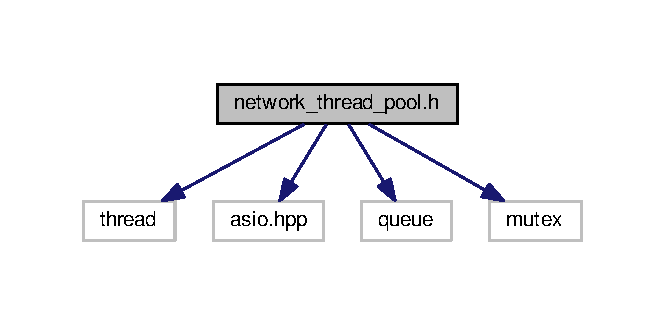
\includegraphics[width=319pt]{network__thread__pool_8h__incl}
\end{center}
\end{figure}
This graph shows which files directly or indirectly include this file\+:\nopagebreak
\begin{figure}[H]
\begin{center}
\leavevmode
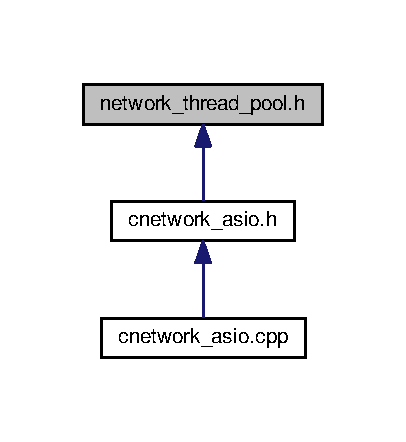
\includegraphics[width=195pt]{network__thread__pool_8h__dep__incl}
\end{center}
\end{figure}
\subsection*{Classes}
\begin{DoxyCompactItemize}
\item 
class \hyperlink{classCore_1_1NetworkThreadPool}{Core\+::\+Network\+Thread\+Pool}
\end{DoxyCompactItemize}
\subsection*{Namespaces}
\begin{DoxyCompactItemize}
\item 
 \hyperlink{namespaceCore}{Core}
\end{DoxyCompactItemize}

\hypertarget{riterator_8h}{}\section{riterator.\+h File Reference}
\label{riterator_8h}\index{riterator.\+h@{riterator.\+h}}
{\ttfamily \#include $<$iterator$>$}\\*
Include dependency graph for riterator.\+h\+:\nopagebreak
\begin{figure}[H]
\begin{center}
\leavevmode
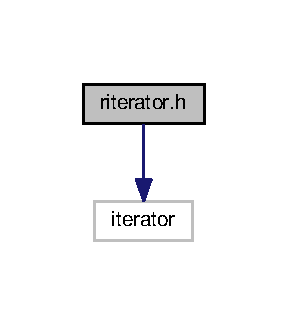
\includegraphics[width=138pt]{riterator_8h__incl}
\end{center}
\end{figure}
\subsection*{Classes}
\begin{DoxyCompactItemize}
\item 
class \hyperlink{classCore_1_1RIterator}{Core\+::\+R\+Iterator$<$ T $>$}
\end{DoxyCompactItemize}
\subsection*{Namespaces}
\begin{DoxyCompactItemize}
\item 
 \hyperlink{namespaceCore}{Core}
\end{DoxyCompactItemize}

%--- End generated contents ---

% Index
\backmatter
\newpage
\phantomsection
\clearemptydoublepage
\addcontentsline{toc}{chapter}{Index}
\printindex

\end{document}
